% ---------- SETUP ----------

\documentclass[11pt, fleqn]{article}

%-------------------------------
%           PACKAGES
%-------------------------------

\usepackage[american]{babel}
\usepackage[usenames,dvipsnames]{xcolor}
\usepackage{multicol}
\usepackage{multirow}
\usepackage{wrapfig}
\usepackage{float}
\usepackage{siunitx}
\usepackage{subfig}
\usepackage{graphicx}
\usepackage{adjustbox}
\usepackage{array}
\usepackage{appendix}
\usepackage{amsmath,amsfonts,amsthm,amssymb}
\usepackage[utf8]{inputenc}
\usepackage{units}
\usepackage{verbatim}
\usepackage{verbdef}  
\usepackage{colortbl}
\usepackage{nicefrac}
\usepackage{physics}
\usepackage{array}
\usepackage{setspace}
\usepackage{fancyhdr}
\usepackage{lastpage}
\usepackage{dsfont}
\usepackage{extramarks}
\usepackage{chngpage}
\usepackage{titlesec}
\usepackage{soul}
\usepackage{tensor}
\usepackage{ifthen}
\usepackage{listings}
\usepackage{courier}
\usepackage{slashed}
\usepackage{cancel}
\usepackage{bbold}
\usepackage[
    labelsep=endash
    ]{caption}
\usepackage[
    top=1.5cm,
    bottom=1.5cm,
    left=2cm,
    right=2cm
    ]{geometry}
\usepackage[
    colorlinks,
    bookmarks=false,
    linkcolor=RedViolet,
    urlcolor=Peach,
    citecolor=TealBlue
    ]{hyperref}
\usepackage[
    backend=biber,
    style=numeric-comp,
    sorting=none,
    isbn=false,
    url=false,
    doi=false
    ]{biblatex}
\usepackage[
    noabbrev
    ]{cleveref}


\usepackage{newpxtext}
\usepackage[defaultsans]{lato}
\linespread{1.02}

%-------------------------------
%           COMMANDS
%-------------------------------

\makeatletter
    \@ifpackageloaded{babel}
    {\addto\extrasamerican{
        \renewcommand*{\figureautorefname}{Figure}
        \renewcommand*{\tableautorefname}{Table}
        \renewcommand*{\partautorefname}{Part}
        \renewcommand*{\chapterautorefname}{Chapter}
        \renewcommand*{\sectionautorefname}{Section}
        \renewcommand{\figurename}{\bfseries\sffamily Figure}
        \renewcommand{\tablename}{\bfseries\sffamily Table}
        }
        \providecommand{\subfigureautorefname}{\figureautorefname}
    }{\relax}
\makeatother

\def \be {\begin{equation}}
\def \ee {\end{equation}}
\def \mc {\mathcal}
\def \one {\mathbb 1}
\def \electron {$e^-$ }

\setcounter{MaxMatrixCols}{20}

\newbibmacro{string+doi}[1]{%
  \iffieldundef{doi}{#1}{\href{http://doi.org/\thefield{doi}}{#1}}}
\DeclareFieldFormat*{title}{\usebibmacro{string+doi}{\mkbibemph{#1}}}
\DeclareFieldFormat*{title}{\usebibmacro{string+doi}{\mkbibquote{#1}}}
\renewbibmacro{in:}{}
\AtEveryBibitem{%
  \clearfield{note}
  \clearfield{pages}
  \clearfield{issue}
  \clearfield{number}
  \clearfield{month}}
\addbibresource{chapters/bib.bib}

% ---------- DOCUEMENT ----------

\begin{document}
\titleformat{\section}{\centering\Huge\bfseries\sffamily\color{RedViolet}}{}{0em}{\MakeUppercase}{}
\titleformat{\subsection}{\Large\bfseries\sffamily\color{RedViolet}}{\hspace{0.5cm}{\color{gray}\textbar}\hspace{0.2cm}}{0em}{}{}

\begin{titlepage}
    \begin{center}    

        \mbox{}    
        \vspace{2cm}
        \begin{center}
            \rule{8cm}{1pt}
        \end{center}
        \vspace{1cm}
        {\Huge\sffamily\color{RedViolet} 1D Chain of Majorana Fermions}
        \vspace{0.7cm}
        \begin{center}
            \rule{8cm}{1pt}
        \end{center}
        \vspace{5 cm}
        
        {\Large\sffamily Anthony REY}\\        
        \vspace{0.5cm}
        {\large\sffamily\textbf{With great help of} Mithilesh NAYAK, Samuel NYCKEES, Zakaria JOUINI}\\

        \vspace{6cm}
        {\sffamily TP IV Project --- PHYS-422}\\
        {\sffamily \'Ecole Polyetchnique Fédérale de Lausanne}

        \vfill
        
\includegraphics[scale=0.03]{../images/logo.png}
        
    \end{center}
\end{titlepage}

\tableofcontents

% \clearpage
\section{Introduction}
% \clearpage
\section{Models}	

	\subsection{Transverse-Field Ising}	

		The Transverse-Field Ising (TFI) model for spin-$1/2$ will be used as a benchmark of the simulations. It is defined for a chain of length $L$ with open boundary conditions as
		\be \mc H = - J \sum_j \sigma^x_j \sigma^x_{j+1} - h \sum_j \sigma^z_j \label{eq:TFI} \ee
		where it is made implicit that 
		\be \sigma^\alpha_j = \underbrace{\one \otimes \cdots \otimes \one}_{j-1} \otimes \sigma^\alpha \otimes \underbrace{\one \otimes \cdots \otimes \one}_{L-j} \ee
		with $\sigma^\alpha$ is the Pauli matrix for $\alpha=x,y,z$. This model undergoes a quantum phase transition at critical point $J=\pm h$. Here, only $J, h > 0$ will be considered.

	\subsection{O'Brien and Fendley}

		The model which shall be mainly studied is the one that will be called O'Brien and Fendley \cite{obrien2018} (OF) model for convenience. For open boundary conditions systems of $L$ spin-$1/2$, the Hamiltonian is written
		\be \mc H = 2\lambda_I\mc H_I + \lambda_3\mc H_3 + \lambda_c\mc H_c \ee
		where
		\be \begin{cases} \mc H_I = i\sum_a \gamma_a \gamma_{a+1} \\ \mc H_3 = - \sum_a \gamma_{a-2}\gamma_{a-1}\gamma_{a+1}\gamma_{a+2} \\ \mc H_c = -i \sum_a \gamma_a\gamma_{a+2} \end{cases} \ee
		It involves the Majorana fermion operators $\gamma_a$ being hermitian $\gamma_a = \gamma_a^\dagger$ and satisfying the Clifford algebra $\{\gamma_a, \gamma_b\} = 2\delta_{ab}$.

		It is more convenient for spin-$1/2$ systems to write their Hamiltonian in terms of Pauli operators. To perform this mapping, the Jordan-Wigner transformation will be of interest.

		It can be noted that the Majorana fermions can be defined in terms of fermionic creation $c^\dagger_j$ and annihilation $c_j$ operators on site $j$ as
		\be \gamma_{2j-1} \equiv c_j + c^\dagger_j \qq{and} \gamma_{2j} \equiv i(c^\dagger_j-c_j) \label{eq:defMajo} \ee
		It is straightforward to show that the choice \eqref{eq:defMajo} satisfies the properties of Majorana fermions. Indeed
		\be \begin{aligned} \gamma^\dagger_{2j-1} &= c^\dagger_j + c_j = c_j + c^\dagger_j \\ &= \gamma_{2j-1} \\ \gamma^\dagger_{2j} &= -i(c_j - c^\dagger_j) = i(c^\dagger_j - c_j) \\ &= \gamma_{2j} \end{aligned} \ee
		and noticing that the fermionic operators respect the anticommutation relations
		\be \{c_i,c^\dagger_j\} = \delta_{ij} \qq{and} \{c_i,c_j\}=\{c^\dagger_i,c^\dagger_j\} = 0 \label{eq:fermionComm} \ee
		the following holds
		\be \begin{aligned} 
			\{\gamma_{2j-1}, \gamma_{2j-1}\} &= \{c_j + c^\dagger_j, c_j + c^\dagger_j\} = \{c^\dagger_j,c_j\} + \{c_j,c^\dagger_j\} \\ &= 2 \\ 
			\{\gamma_{2j}, \gamma_{2j}\} &= \{i(c^\dagger_j-c_j), i(c^\dagger_j-c_j)\} = -\{c^\dagger_j, -c_j\} - \{-c_j, c^\dagger_j\} \\ &= 2 \\
			\{\gamma_{2j-1}, \gamma_{2j}\} &= \{c_j + c^\dagger_j, i(c^\dagger_j-c_j)\} = -i\{c^\dagger_j, c_j\} +i \{c_j, c^\dagger_j\} \\ &= 0
		\end{aligned} \ee
		meaning that the Clifford algebra is satisfied.

		Now the goal is to map the fermionic operators onto the Pauli operators, and this mapping is the Jordan-Wigner transformation. Recall the commutation relations for the Pauli operators
		\be [\sigma^\alpha_i, \sigma^\beta_j] = 2i\delta_{ij}\varepsilon_{\alpha\beta\gamma} \sigma^\gamma_j \qq{and} \{\sigma^\alpha_j, \sigma^\beta_j\} = 2\delta_{\alpha\beta} \label{eq:pauliComm} \ee
		Defining $\sigma^\pm_j \equiv \frac 1 2 (\sigma^x_j \pm i\sigma^y_j)$, \eqref{eq:pauliComm} give on the same site
		\be \{\sigma^+_j, \sigma^-_j\} = 1 \qq{and} \{\sigma^+_j, \sigma^+_j\} = \{\sigma^-_j, \sigma^-_j\} = 0 \label{eq:qubitAnti} \ee
		an on different sites
		\be [\sigma^+_i, \sigma^-_j] = 0 \qq{and} [\sigma^+_i, \sigma^+_j] = [\sigma^-_i, \sigma^-_j] = 0 \quad \forall i\neq j \label{eq:qubitComm} \ee
		This is the anticommutation relation for fermionic operators on the same site. It is convenient to define operators $b_j$ and $b^\dagger_j$ as
		\be \sigma^+_j \equiv b_j \qq{and} \sigma^-_j \equiv b^\dagger_j \ee
		Hence, $\{b_j,b^\dagger_j\} = 1$. Introduce the writing
		\be b_j = e^{i\pi\sum_{k=1}^{j-1} c^\dagger_k c_k}c_j \qq{and} b^\dagger_j = e^{-i\pi\sum_{k=1}^{j-1} c^\dagger_k c_k}c^\dagger_j \label{eq:defb} \ee
		and define for simplicity
		\be J_j \equiv e^{i\pi\sum_{k=1}^{j-1} c^\dagger_k c_k} \ee
		Few properties will be important
		\begin{align}
			&\bullet \ J^\dagger_j = J_j \label{eq:propJ1} \\
			&\bullet \ \textstyle J_j = \prod_{k=1}^{j-1} (1-2c^\dagger_k c_k) \label{eq:propJ2} \\
			&\bullet \ J^2_j = \one \label{eq:propJ3} \\
			&\bullet \ [J_i,c_j] = [J_i, c^\dagger_j] =0 \quad \forall i\leq j \label{eq:propJ4}
		\end{align}
		To prove \eqref{eq:propJ1}, note that $c^\dagger_k c_k \in \{0,1\}$, then $\sum_{k=1}^{j-1} c^\dagger_k c_k \in \mathbb N$. This implies that, $J^\dagger_j = e^{-in\pi} = e^{in\pi} = J_j$ for $n \in \mathbb N$.\\
		To prove \eqref{eq:propJ2}, recall that $c^\dagger_k c_k \in \{0,1\}$ then $e^{i\pi\sum_{k=1}^{j-1} c^\dagger_k c_k} = \prod_{k=1}^{j-1} e^{i\pi c^\dagger_k c_k}$. Since
		\be e^{i\pi c^\dagger_k c_k} = \begin{cases} 1 & \text{if } c^\dagger_k c_k = 0 \\ -1 & \text{if } c^\dagger_k c_k = 1 \end{cases} \implies e^{i\pi c^\dagger_k c_k} = 1-2c^\dagger_k c_k \ee
		To prove \eqref{eq:propJ3}, simply notice that using $c_k c^\dagger_k = 1-c^\dagger_k c_k$
		\be \begin{split} (1-2c^\dagger_k c_k)^2 &= 1 - 4c^\dagger_k c_k + 4c^\dagger_k c_k c^\dagger_k c_k = 1 -4 c^\dagger_k c_k + 4c^\dagger_k c_k \\ &= 1 \end{split} \ee
		To prove \eqref{eq:propJ4}, it suffices to recall that every fermionic operator anticommute with any other one on different sites. Since $J_i$ involves only operators $c^\dagger_k c_k \ \forall k<i$, passing any $c_j, c^\dagger_j$ across $J_i$ costs a factor $(-1)^2=1$.
		These allow to write
		\be \begin{split} b^\dagger_j b_j &= c^\dagger_j J^\dagger J_j c_j = c^\dagger J^
		2_j c_j \\ &= c^\dagger_j c_j \end{split} \label{eq:bbcc} \ee

		Now remains to prove that the definition \eqref{eq:defb} gives the correct anticommutation relations \eqref{eq:qubitAnti} on the same site and commutation relations \eqref{eq:qubitComm} on different sites. On the same site
		\be \begin{aligned} 
			\{b_j, b^\dagger_j\} &= b_j b^\dagger_j + b^\dagger_j b_j = c_j c^\dagger_j + c^\dagger_j c_j = 1 \\
			\{b_j, b_j\} &= 2 b_j b_j = 2 J_jc_jJ_jc_j = 2 c_jc_j = 0 \\
			\{b^\dagger_j, b^\dagger_j\} &= 2 b^\dagger_j b^\dagger_j = 2 c^\dagger_jJ^\dagger_jc^\dagger_jJ^\dagger_j = 2 c^\dagger_jc^\dagger_j = 0 
		\end{aligned} \ee
		On different sites, assuming without loss of generality $i<j$, 
		\be \begin{aligned}
			b_i b^\dagger_j &= c_i c^\dagger_j e^{-i\pi\sum_{k=i}^{j-1} c^\dagger_k c_k} \\
			b^\dagger_j b_i &= c^\dagger_j e^{-i\pi\sum_{k=i}^{j-1} c^\dagger_k c_k} c_i
		\end{aligned} \ee
		Here, passing $c_i$ to the left is no longer straightforwardly free. The term in the exponential $c^\dagger_i c_i =0$ since any spin on site $i$ is killed by the $c_i$ on the right. If the $c_i$ is passed to the left of the exponential, then $c^\dagger_i c_i =1$ since otherwise the whole term would have vanished by the application of $c_i$ on the right. This passage implies a factor $e^{-i\pi} = -1$. Then passing $c_i$ to the left of $c^\dagger_j$ costs another factor $-1$, which means $b_i b^\dagger_j = b^\dagger_j b_i$. Then, performing the same operations and noticing that also $c^\dagger_i$ enforces $c^\dagger_i c_i =1$, whereas when passed to the left, the term in exponential is $c^\dagger_i c_i =0$, since states with $c^\dagger_i c_i =1$ vanish under application of $c^\dagger_i$, 
		\be \begin{aligned}
			b_i b_j &= c_i c_j e^{2i\pi\sum_{k=1}^{i-1} c^\dagger_k c_k + i\pi\sum_{k=i}^{j-1} c^\dagger_k c_k} = b_j b_i \\
			b^\dagger_i b^\dagger_j &= c^\dagger_i c^\dagger_j e^{-2i\pi\sum_{k=1}^{i-1} c^\dagger_k c_k - i\pi\sum_{k=i}^{j-1} c^\dagger_k c_k} = b^\dagger_j b^\dagger_i
		\end{aligned} \ee
		Therefore
		\be [b_i, b^\dagger_j] = 0, \qq{and} [b_i, b_j] = [b^\dagger_i, b^\dagger_j] = 0 \quad \forall i\neq j \ee
		Finally, it remains to check the commutation relation on the same site. For the spin operators
		\be \begin{split} [\sigma^+_j, \sigma^-_j] &= \frac 1 4 [\sigma^x_j+i\sigma^y_j, \sigma^x_j-i\sigma^y_j] = -\frac i 2 [\sigma^x_j,\sigma^y_j] \\ &= \sigma^z_j \end{split} \ee
		For the definition \eqref{eq:defb}
		\be [b_j, b^\dagger_j] = c_j c^\dagger_j - c^\dagger_j c_j = 1 - 2c^\dagger_j c_j \ee
		and recalling that by definition
		\be \sigma^x_j = b_j + b^\dagger_j \qq{and} \sigma^y_j = i(b^\dagger_j - b_j) \ee
		if appears that
		\be \begin{split} [\sigma^x_j,  \sigma^y_j] &= [b_j + b^\dagger_j, b^\dagger_j - b_j] = i[b_j b^\dagger_j - b^\dagger_j b_j - b^\dagger_j b_j + b_j b^\dagger_j] \\ &= 2i(1 - 2 b^\dagger_j b_j) \end{split} \ee
		However, $[\sigma^x_j,  \sigma^y_j]=2i\sigma^z_j$, hence
		\be \sigma^z_j = 1 - 2 b^\dagger_j b_j \ee
		which is what wanted using \eqref{eq:bbcc}. This completes the proof that the operators defined in \eqref{eq:defb} satisfy \eqref{eq:pauliComm}.

		In the end, the Majorana fermion operators can be expressed in terms of the Pauli operators as
		\be \begin{split} \gamma_{2j-1} &= c_j + c^\dagger_j = J_j(b_j + b^\dagger_j) = J_j \sigma^x_j = \textstyle \sigma^x_j \prod_{k=1}^{j-1} (1 - 2c^\dagger_k c_k) \\ \gamma_{2j} &= i(c^\dagger_j - c_j) = iJ_j(b^\dagger_j - b_j) = J_j \sigma^y_j = \textstyle \sigma^x_j \prod_{k=1}^{j-1} (1 - 2c^\dagger_k c_k) \end{split} \ee
		therefore, using \eqref{eq:propJ2}
		\be \gamma_{2j-1} = \sigma^x_j \prod_{k=1}^{j-1} \sigma^z_k \qq{and} \gamma_{2j} = \sigma^y_j \prod_{k=1}^{j-1} \sigma^z_k \ee

		Now, the goal is to express the Hamiltonian in terms of Pauli operators. First, to see the pattern, try to compute
		\be \begin{split} \sigma^x_j \sigma^x_{j+1} &\stackrel{\eqref{eq:propJ4}}{=} (c_j + c^\dagger_j) (c_{j+1} + c^\dagger_{j+1}) J_j J_{j+1} \\ &\stackrel{\eqref{eq:propJ2}}{=} (c_j + c^\dagger_j) (c_{j+1} + c^\dagger_{j+1}) \textstyle \prod_{k=1}^{j-1} (1-2c^\dagger_k c_k)^2 (1-2c^\dagger_j c_j) \\ &= (c_jc_{j+1} + c_jc^\dagger_{j+1} + c^\dagger_j c_{j+1} + c^\dagger_j c^\dagger_{j+1}) (1-2c^\dagger_j c_j) \\ &\stackrel{\eqref{eq:fermionComm}}{=} c_jc_{j+1} + 2c_{j+1} c_j + c_jc^\dagger_{j+1} + 2c^\dagger_{j+1}c_j + c^\dagger_j c_{j+1} + c^\dagger_j c^\dagger_{j+1} \\ &\stackrel{\eqref{eq:fermionComm}}{=} -c_jc_{j+1} - c_jc^\dagger_{j+1} + c^\dagger_j c_{j+1} + c^\dagger_j c^\dagger_{j+1} \\ &= (c^\dagger_j -c_j)(c_{j+1} + c^\dagger_{j+1}) \\ &\stackrel{\eqref{eq:defMajo}}{=} -i\gamma_{2j}\gamma_{2j+1} \end{split} \ee 
		Also, 
		\be \begin{split} \gamma_{2j}\gamma_{2j+1} &= i (c_j + c^\dagger_j)(c^\dagger_j -c_j) = i(c_jc^\dagger_j - c^\dagger_j c_j) = i(1-2c^\dagger_j c_j) \\ &= i \sigma^z_j \\ \implies \sigma^z_j &= -i\gamma_{2j-1}\gamma_{2j} \end{split} \ee
		Noticing the possibility to split $\sum_a = \sum_{a\text{ even}} + \sum_{a\text{ odd}}$ allows to write 
		\be \mc H_I = -\sum_j \sigma^x_j \sigma^x_{j+1} - \sum_j \sigma^z_j \ee
		The identification $\gamma_a \gamma_{a+1} \rightarrow \gamma_{2j-1}\gamma_{2j} + \gamma_{2j}\gamma_{2j+1}$ enables to express
		\be \begin{split} \gamma_{a-2}\gamma_{a-1}\gamma_{a+1}\gamma_{a+2} &\rightarrow \gamma_{2j-3}\gamma_{2j-2}\gamma_{2j}\gamma_{2j+1} + \gamma_{2j-2}\gamma_{2j-1}\gamma_{2j+1}\gamma_{2j+2} \\ &= i\sigma^z_{j-1} i\sigma^x_j\sigma^x_{j+1} + i\sigma^x_{j-1}\sigma^x_j i\sigma^z_{j+2} \\ &\xrightarrow{j\rightarrow j+1} -\sigma^z_j\sigma^x_{j+1}\sigma^x_{j+2} -\sigma^x_j\sigma^x_{j+1}\sigma^z_{j+2} \end{split} \ee
		Therefore
		\be \mc H_3 = \sum_j \sigma^z_j\sigma^x_{j+1}\sigma^x_{j+2} + \sum_j \sigma^x_j\sigma^x_{j+1}\sigma^z_{j+2} \ee
		Finally, with $\gamma_a \gamma_{a+2} \rightarrow \gamma_{2j}\gamma_{2j+2} + \gamma_{2j-1}\gamma_{2j+1}$
		\be \begin{split} \gamma_{2j-1}\gamma_{2j+1} &= (c_j + c^\dagger_j) (c_{j+1} + c^\dagger_{j+1}) \\ &= c_jc_{j+1} + c_jc^\dagger_{j+1} + c^\dagger_j c_{j+1} + c^\dagger_j c^\dagger_{j+1} \\ &= (-c_jc_{j+1} + -c_jc^\dagger_{j+1} + c^\dagger_j c_{j+1} + c^\dagger_j c^\dagger_{j+1}) (1 - 2c^\dagger_j c_j) \\ &= (c^\dagger_j - c_j) (c_{j+1} + c^\dagger_{j+1}) J_j J_{j+1} \\ &= -i\sigma^y_j \sigma^x_{j+1} \\ \implies \sigma^y_j \sigma^x_{j+1} &= i\gamma_{2j-1}\gamma_{2j+1} \end{split} \ee
		and doing the same
		\be \begin{split} \gamma_{2j}\gamma_{2j+2} &= -(c^\dagger_j - c_j) (c^\dagger_{j+1} - c_{j+1}) \\ &= -(c^\dagger_j c^\dagger_{j+1} - c^\dagger_j c_{j+1} - c_jc^\dagger_{j+1} + c_jc_{j+1}) \\ &= -(c^\dagger_j c^\dagger_{j+1} - c^\dagger_j c_{j+1} + c_jc^\dagger_{j+1} - c_jc_{j+1}) (1 - 2c^\dagger_j c_j) \\ &= -(c_j + c^\dagger_j) (c^\dagger_{j+1} - c_{j+1}) J_j J_{j+1} \\ &= i\sigma^x_j \sigma^x_{j+1} \\ \implies \sigma^x_j \sigma^y_{j+1} &= -i\gamma_{2j}\gamma_{2j+2} \end{split} \ee
		This implies
		\be \mc H_c = \sum_j \sigma^x_j\sigma^y_{j+1} - \sum_j \sigma^y_j\sigma^y_{j+1} \ee

		To sum up, the OF model is
		\be \mc H = - 2\lambda_I \sum_j [\sigma^x_j \sigma^x_{j+1} + \sigma^z_j] + \lambda_3 \sum_j [\sigma^z_j\sigma^x_{j+1}\sigma^x_{j+2} + \sigma^x_j\sigma^x_{j+1}\sigma^z_{j+2}] + \lambda_c \sum_j [\sigma^x_j\sigma^y_{j+1} - \sigma^y_j\sigma^y_{j+1}] \label{eq:OF} \ee
% \clearpage
\section{Method}

	The algorithm that will be used is the finite-size Density Matrix Renormalization Group (DRMG) with $2$-site update. It follows almost to the letter the method described in \cite{schollwoeck2011}.

	Everything will be coded in python language, from scratch, except for 
	\begin{itemize}
		\item the contraction of tensors for which a very convenient function called \verb_ncon_ \cite{pfeifer2015} for python will be used, which wraps the \verb_numpy.tensordot_ into an intuitive way.
		\item the SVD routine for which \verb_numpy.linalg.svd_ will be used.
		\item the diagonalization routine of the effective Hamiltonian whenever it requires excitation energies to be found for which ARPACK \cite{lehoucq1998} implemented in \verb_scipy.sparse.linalg.eigen.arpack_ will be used.
	\end{itemize}

	\subsection{Brief recall on DMRG}

        The finite-size DMRG is summarized in \eqref{eq:dmrgSum}. The growth process of \emph{eg} block $B$ is done at the expense of block $A$, which shrinks \emph{ie} old shorter blocks $A$ are reused. This is continued until $A$ is so small as to have a complete Hilbert space. Then the growth direction is reversed. $A$ grows at the expense of $B$, including new ground state determinations and basis choices for $A$, until $B$ is small enough to have a complete Hilbert space, which leads to yet another reversal of growth direction. This sweeping through the system is continued until energy converges. The intuitive motivation for this procedure is that after each sweep, blocks $A$ or $B$ are determined in the presence of an ever improved embedding.
        
        The ground state can be found using an iterative method by minimizing the energy $E = \frac{\ev{\mc H}{\psi}}{\braket{\psi}}$ thus finding
        \be \min_{\ket \psi, \lambda} \ev{\mc H}{\psi} - \lambda\braket{\psi} \ee
        The problem is that if one considers all the matrices $M$, the problem is highly non-linear. But one can proceed by keeping all the matrices on the sites except the one considered fixed. Of course, this is computationally worth --- quadratic form --- but not optimal. To calculate the terms of the minimization, note that it can be recast into a generalized eigenvalue problem
        \be \mc H v - \lambda \mc N v =0 \ee
        with $v_{\sigma_\ell,a_{\ell-1},a_\ell} = M^{\sigma_\ell}_{a_{\ell-1},a_\ell}$. If $\ket\psi$ is mixed canonical, thus left-normalized at the left of the site $\ell$ and right-normalized on the right, then $\mc N = \mathbb 1$, so that the problem reduces to a standard eigenvalue problem.

        The algorithm is as follows
        \begin{itemize}
            \item start for a random $\ket \psi$ made of the matrices $M^{\sigma_\ell}$
            \item right-normalize it, \emph{ie} write it a product a right-orthonormal matrices $B^{\sigma_\ell}$ 
            \item run the optimization from $\ell=1$ to $L-1$, that is, solve the eigenvalue problem for $M^{\sigma_\ell}$, then left-normalize it to $A^{\sigma_\ell}$ by SVD, absorb the $SV^\dagger$ into the $M^{\sigma_{\ell+1}}$, then move to the $\ell+1$ site and repeat until $L-1$
            \item start from $\ell = L$ to 2, and do the same but right-normalizing
            \item repeat the sweeps until convergence, but can fall in local minimum thus seek for the null error on the energy
        \end{itemize}

        \be \begin{split} &M_0 B_0 B_0 B_0 \cdots B_0 \\ \xrightarrow{\text{optimize}} &M_1 B_0 B_0 B_0 \cdots B_0 \xrightarrow{\text{SVD}} A_1 M_0 B_0 B_0 \cdots B_0 \\ \xrightarrow{\text{optimize}} &A_1 M_1 B_0 B_0 \cdots B_0 \xrightarrow{\text{SVD}} A_1 A_1 M_0 B_0 \cdots B_0 \\ \xrightarrow{\text{optimize}} &A_1 A_1 M_1 B_0 \cdots B_0 \xrightarrow{\text{SVD}} A_1 A_1 A_1 M_0 \cdots B_0 \\ \xrightarrow{\cdots} &A_1 A_1 A_1 A_1 \cdots M_0 \\ \xrightarrow{\text{optimize}}  &A_1 A_1 A_1 A_1 \cdots M_1 \xrightarrow{\text{SVD}} A_1 A_1 A_1 A_1 \cdots B_1 \\ \xrightarrow{\cdots} &A_1 A_1 A_1 M_1 \cdots B_1 \\ \xrightarrow{\text{optimize}} &A_1 A_1 A_1 M_2 \cdots B_1 \xrightarrow{\text{SVD}} A_1 A_1 M_1 B_2 \cdots B_1 \\ \xrightarrow{\text{optimize}} &A_1 A_1 M_2 B_2 \cdots B_1 \xrightarrow{\text{SVD}} A_1 M_1 B_2 B_2 \cdots B_1 \\ \xrightarrow{\text{optimize}} &A_1 M_2 B_2 B_2 \cdots B_1 \xrightarrow{\text{SVD}} M_1 B_2 B_2 B_2 \cdots B_1 \\ \xrightarrow{\cdots} & \end{split} \label{eq:dmrgSum} \ee

	\subsection{MPO construction for OBCs and free at both edges}
		
		Here, the open boundary conditions (OBCs) with states at both edges of the chain, denoted as $[ff]$ will be of interest.

		For simplicity, since in OF model \eqref{eq:OF} there is the critical $J=h$ TFI model \eqref{eq:TFI}, the former will be slightly modified by adding the $J$ and $h$ couplings appearing in TFI to only make use of one MPO that allows to switch between the different model just by tuning the different coefficients. The Hamiltonian is therefore
		\be \mc H = - 2\lambda_I \sum_j [J\sigma^x_j \sigma^x_{j+1} + h\sigma^z_j] + \lambda_3 \sum_j [\sigma^z_j\sigma^x_{j+1}\sigma^x_{j+2} + \sigma^x_j\sigma^x_{j+1}\sigma^z_{j+2}] + \lambda_c \sum_j [\sigma^x_j\sigma^y_{j+1} - \sigma^y_j\sigma^y_{j+1}] \label{eq:modifiedOF} \ee

		To construct the MPO representing \eqref{eq:modifiedOF} in the bulk, only consider one term in the sum over $j$, namely $j=\ell$. Looking at the string of operators from its right end, the action of each operator on each bond moves the string into a new state, whose label correspond to the string of operators on the right of the bond considered. Then the typical action of the term $\ell$ is viewed as
		\be \arraycolsep=1.5pt \begin{array}{llclclcll}
			\cdots &\one \stackrel{7}{\otimes} \one \stackrel{7}{\otimes} &-2\lambda_I h \sigma^z &\stackrel{1}{\otimes} &\one &\stackrel{1}{\otimes} &\one &\stackrel{1}{\otimes} \one &\cdots \\
			\cdots &\one \stackrel{7}{\otimes} \one \stackrel{7}{\otimes} &-2\lambda_I J \sigma^x &\stackrel{2}{\otimes} &\sigma^x &\stackrel{1}{\otimes} &\one &\stackrel{1}{\otimes} \one &\cdots \\
			\cdots &\one \stackrel{7}{\otimes} \one \stackrel{7}{\otimes} &\lambda_3 \sigma^z &\stackrel{4}{\otimes} &\sigma^x &\stackrel{2}{\otimes} &\sigma^x &\stackrel{1}{\otimes} \one &\cdots \\
			\cdots &\one \stackrel{7}{\otimes} \one \stackrel{7}{\otimes} &\lambda_3 \sigma^x &\stackrel{5}{\otimes} &\sigma^x &\stackrel{3}{\otimes} &\sigma^z &\stackrel{1}{\otimes} \one &\cdots \\
			\cdots &\one \stackrel{7}{\otimes} \one \stackrel{7}{\otimes} &\lambda_c \sigma^x &\stackrel{6}{\otimes} &\sigma^y &\stackrel{1}{\otimes} &\one &\stackrel{1}{\otimes} \one &\cdots \\
			\cdots &\one \stackrel{7}{\otimes} \one \stackrel{7}{\otimes} &\lambda_c \sigma^y &\stackrel{2}{\otimes} &\sigma^x &\stackrel{1}{\otimes} &\one &\stackrel{1}{\otimes} \one &\cdots
		\end{array} \ee
		where the states have been labeled following \autoref{tab:statesOF}.

		\begin{table}[h!]
			\centering
			\begin{tabular}{lcl}
				\hline
				1 & --- & $\one$ \\
				2 & --- & $\sigma^x$ \\
				3 & --- & $\sigma^z$ \\
				4 & --- & $\sigma^x \otimes \sigma^x$ \\
				5 & --- & $\sigma^x \otimes \sigma^z$ \\
				6 & --- & $\sigma^y$ \\
				7 & --- & completed interaction \\
				\hline
			\end{tabular}
			\caption{Labeling of states involved in the construction of the MPO for the \eqref{eq:modifiedOF} Hamiltonian with open $[ff]$ BCs. Each term corresponds to what is on the right of the bond considered.}
			\label{tab:statesOF}
		\end{table}
		This is encoded in the bulk matrix of the MPO, called $W^{[\ell]}$, whose entries $W_{ij}^{[\ell]}$ correspond to the operator making the transition from the state $j \to i$. The bulk matrix for the Hamiltonian \eqref{eq:modifiedOF} is therefore the $7\times 7$ matrix
		\be W^{[\ell]} = \bmqty{
			\one & \cdot & \cdot & \cdot & \cdot & \cdot & \cdot \\
			\sigma^x & \cdot & \cdot & \cdot & \cdot & \cdot & \cdot \\
			\sigma^z & \cdot & \cdot & \cdot & \cdot & \cdot & \cdot \\
			\cdot & \sigma^x & \cdot & \cdot & \cdot & \cdot & \cdot \\
			\cdot & \cdot & \sigma^x & \cdot & \cdot & \cdot & \cdot \\
			\sigma^y & \cdot & \cdot & \cdot & \cdot & \cdot & \cdot \\
			-2\lambda_I h \sigma^z & -2\lambda_I J \sigma^x - \lambda_c \sigma^y & \cdot & \lambda_3 \sigma^z & \lambda_3 \sigma^x & \lambda_c \sigma^x & \one
			} \ee
		Finally, it remains to find the $W^{[1]}$ and $W^{[L]}$ matrices. This is easily done by noticing that $W^{[1]}$ only enables to complete the unfinished interactions started with $W^{[2]}$ and $W^{[3]}$, then is equal to last row of $W^{[\ell]}$. Similarly, $W^{[L]}$ only serves as a starter of interactions that will be completed with $W^{[L-1]}$ and $W^{[L-2]}$, then is equal to the first column of $W^{[\ell]}$. In the end, they are written
		\be W^{[1]} = \bmqty{-2\lambda_I h \sigma^z \\ -2\lambda_I J \sigma^x - \lambda_c \sigma^y \\ \cdot \\ \lambda_3 \sigma^z \\ \lambda_3 \sigma^x \\ \lambda_c \sigma^x \\ \one}^\top \qq{and} W^{[L]} = \bmqty{\one \\ \sigma^x \\ \sigma^z \\ \cdot \\ \cdot \\ \sigma^y \\ -2\lambda_I h \sigma^z} \ee

	\subsection{MPO construction for OBCs with pinning}
		
		The model presented with $[ff]$ BCs can suffer from entanglement coming from the edge states. Hence, it can be useful to fix their spin. For that purpose, the notation which will be used to denote the BCs is presented on \autoref{tab:pinningBCs}. Moreover, even if everything is expressed in the $z$-basis, the spins will be fixed in the $x$-direction since the TFI \eqref{eq:TFI} is $\mathbb Z_2$-symmetric with respect to flipping all the spins in the $x$-direction. Then the states $\ket \pm$ are introduced as
		\be \sigma^x \ket\pm = \pm \ket \pm \label{eq:xPinDef} \ee
		where $\ket +$ means the spin pointing up and $\ket -$ pointing down in $x$-direction.

		\begin{table}[h!]
			\centering
			\begin{tabular}{rcl}
				\hline
				$[ff]$ & $\sim$ & free at both ends \\
				$[f\pm]$ & $\sim$ & free at left end and $\ket \pm_\text{right}$\\
				$[f\pm]$ & $\sim$ & $\ket \pm_\text{left}$ and free at right end  \\
				$[\pm \pm]$ & $\sim$ & $\ket \pm_\text{left}$ and $\ket \pm_\text{right}$ \\
				\hline
			\end{tabular}
			\caption{Labeling of the different BCs used with the definition of the states in \eqref{eq:xPinDef}.}
			\label{tab:pinningBCs}
		\end{table}

		To fix a spin on a site, it suffices to introduce a pinning field $h_\text{pin}$ in the direction wanted. Therefore, the term $h_\text{pin} \sigma^x$ is added in the Hamiltonian MPO as 
		\be W^{[1]} = \bmqty{-2\lambda_I h \sigma^z {\color{TealBlue}+h_\text{pin}\sigma^x} \\ -2\lambda_I J \sigma^x - \lambda_c \sigma^y \\ \cdot \\ \lambda_3 \sigma^z \\ \lambda_3 \sigma^x \\ \lambda_c \sigma^x \\ \one}^\top \qq{and} W^{[L]} = \bmqty{\one \\ \sigma^x \\ \sigma^z \\ \cdot \\ \cdot \\ \sigma^y \\ -2\lambda_I h \sigma^z {\color{TealBlue}+h_\text{pin}\sigma^x}} \ee
		where the bulk $W^{[\ell]}$, $\ell\in]1, L[$ remain the same.

	\subsection{MPO construction for PBCs}

		It will be useful to use DMRG with an Hamiltonian with periodic boundary conditions (PBCs). This would remove the edge states that would be present in the free OBCs and might still be in the fixed OBCs. However, PBCs DMRG in the MPS formalism suffers from problems \cite{schollwoeck2011}, and several ideas have been put on the stage to cope with them \cite{dey2016, pippan2010, verstraete2004, pirvu2011}, and the main issue that arises when the goal is not to drastically change the way the DMRG was coded, is that to get the same precision on the targeted ground state with OBCs and PBCs, the bond dimension $\chi$ in OBCs has to be increased to $\chi^2$ in PBCs \cite{schollwoeck2011}. Nonetheless, these issues will not be taken into account here, but the the generalized eigenvalue problem arising from naively taking the trace of the MPS to represent PBCs will be solved by folding the MPS as in \autoref{fig:foldMPS}.

		\begin{figure}[h!]
			\centering
			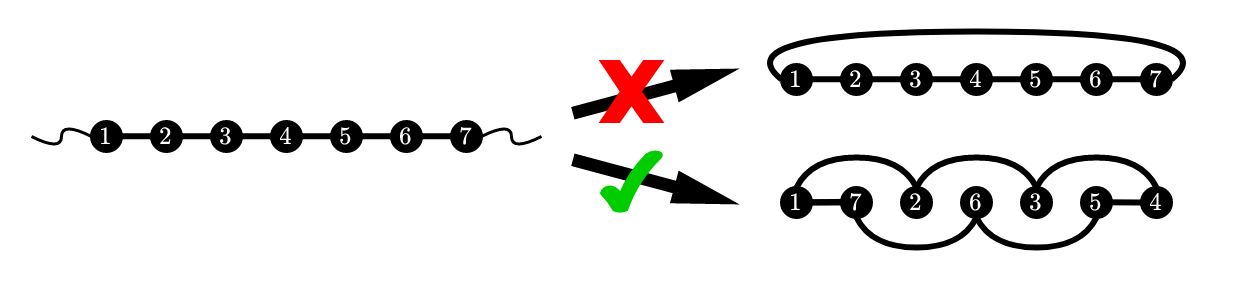
\includegraphics[scale=0.4]{../images/pbcmps.png}
			\caption{Way to represent the MPS in OBCs and its extension to PBCs, where nearest-neighbor couplings become second-nearest-neighbor ones, here presented with 7 sites.}
			\label{fig:foldMPS}
		\end{figure}

		This way to represent the MPS only amounts to change the MPO used. However, one must be very careful when deriving it, as many of the terms in \eqref{eq:OF} appearing at the edges change in a non-trivial way. Noticing that $\lambda_c=0$ will be taken to simplify here, the bulk is becoming the $15\times15$ matrix
		\be W^{[\ell]} = \bmqty{
			\one & \cdot & \cdot & \cdot & \cdot & \cdot & \cdot & \cdot & \cdot & \cdot & \cdot & \cdot & \cdot & \cdot & \cdot \\
			\sigma^x & \cdot & \cdot & \cdot & \cdot & \cdot & \cdot & \cdot & \cdot & \cdot & \cdot & \cdot & \cdot & \cdot & \cdot \\
			\sigma^z & \cdot & \cdot & \cdot & \cdot & \cdot & \cdot & \cdot & \cdot & \cdot & \cdot & \cdot & \cdot & \cdot & \cdot \\
			\cdot & \one & \cdot & \cdot & \cdot & \cdot & \cdot & \cdot & \cdot & \cdot & \cdot & \cdot & \cdot & \cdot & \cdot \\
			\cdot & \cdot & \one & \cdot & \cdot & \cdot & \cdot & \cdot & \cdot & \cdot & \cdot & \cdot & \cdot & \cdot & \cdot \\
			\cdot & \cdot & \cdot & \cdot & \cdot & \cdot & \cdot & \cdot & \cdot & \cdot & \cdot & \cdot & \cdot & \cdot & \cdot \\
			\cdot & \cdot & \cdot & \cdot & \cdot & \cdot & \cdot & \cdot & \cdot & \cdot & \cdot & \cdot & \cdot & \cdot & \cdot \\
			\cdot & \cdot & \cdot & \sigma^x & \cdot & \cdot & \cdot & \cdot & \cdot & \cdot & \cdot & \cdot & \cdot & \cdot & \cdot \\
			\cdot & \cdot & \cdot & \cdot & \sigma^x & \cdot & \cdot & \cdot & \cdot & \cdot & \cdot & \cdot & \cdot & \cdot & \cdot \\
			\cdot & \cdot & \cdot & \cdot & \cdot & \cdot & \cdot & \cdot & \cdot & \cdot & \cdot & \cdot & \cdot & \cdot & \cdot \\
			\cdot & \cdot & \cdot & \cdot & \cdot & \cdot & \cdot & \cdot & \cdot & \cdot & \cdot & \cdot & \cdot & \cdot & \cdot \\
			\cdot & \cdot & \cdot & \cdot & \cdot & \cdot & \cdot & \one & \cdot & \cdot & \cdot & \cdot & \cdot & \cdot & \cdot \\
			\cdot & \cdot & \cdot & \cdot & \cdot & \cdot & \cdot & \cdot & \one & \cdot & \cdot & \cdot & \cdot & \cdot & \cdot \\
			\cdot & \cdot & \cdot & \cdot & \cdot & \cdot & \cdot & \cdot & \cdot & \cdot & \cdot & \cdot & \cdot & \cdot & \cdot \\
			-2\lambda_I h \sigma^z & \cdot & \cdot & -2\lambda_I J \sigma^x & \cdot & \cdot & \cdot & \cdot & \cdot & \cdot & \cdot & \lambda_3 \sigma^z & \lambda_3 \sigma^x & \cdot & \one} \ee
		Now, there are numerous changes to make for the matrices on sites near the boundaries, that are summarized in \autoref{tab:mpoPBCsBoundaries}, where PBCs and antiperiodic boundary conditions (aPBCs) are also given, noticing that aPBCs amount to a change
		\be \sigma^x_L \sigma^x_1 \to - \sigma^x_L \sigma^x_1 \ee

		\begin{table}[h!]
			\centering
			\begin{tabular}{c|lllll}
				$\ell$ & \multicolumn{1}{c}{$1$} &\multicolumn{1}{c}{$2$} & \multicolumn{1}{c}{$L-3$} & \multicolumn{1}{c}{$L-2$} & \multicolumn{1}{c}{$L-1$} \\
				\hline
				\multirow{5}{*}{$W_{ij}^{[\ell]}$ with $(j,i)$} & $(2, 15)$ : $\mp 2\lambda_I J \sigma^x$ & $(2, 14)$ : $\sigma^z$ & $(10, 15)$ : $\lambda_3 \sigma^z$ & $(6, 10)$ : $\one$ & $(2, 6)$ : $\sigma^x$ \\
				& $(7, 15)$ : $\pm \lambda_3 \sigma^x$ & $(3, 7)$ : $\sigma^x$ & $(11, 15)$ : $\lambda_3 \sigma^x$ & $(6, 15)$ : $\lambda_3 \sigma^z$ & $(2, 14)$ : $\sigma^z$ \\
				& $(8, 15)$ : $\lambda_3 \sigma^z$ & & & $(7, 11)$ : $\one$ & $(2, 15)$ : $-2\lambda_I J \sigma^x$ \\
				& $(9, 15)$ : $\pm \lambda_3 \sigma^x$ & & & $(14, 15)$ : $\lambda_3 \sigma^x$ & $(3, 7)$ : $\sigma^x$ \\
				& $(14, 15)$ : $\lambda_3 \sigma^x$ & & & & \\
			\end{tabular}
			\caption{All changes made in the matrices of the MPO for Hamiltonian \eqref{eq:OF} with $\lambda_c=0$ for PBCs and aPBCS respectively.}
			\label{tab:mpoPBCsBoundaries}
		\end{table}
		Finally, once again, $W^{[1]}$ is actually taken to be the last row of $W^{[1]}$ and $W^{[L]}$ the first column of $W^{[L]}$.

	\subsection{Excitation energies}

		DRMG is particularly suited to find the ground state of an Hamiltonian associated to its lowest eigenvalue. However, it is often useful to find the excitation spectrum of the Hamiltonian, or at least its low-lying excitation energies. To this end, one can exploit the property of DRMG to finding the ground state and use an Hamiltonian slightly modified so that the state having a vanishing overlap with the ground state is punished with a large energy, allowing to converge to the state orthogonal to the ground state with the same or higher energy. To be specific, a first DRMG can be run converging to the ground state $\ket{\psi_0}$ of $\mc H$. Then a new DRMG is run with
		\be \tilde{\mc H} = \mc H + \lambda_0 \dyad{\psi_0} \ee 
		with $\lambda_0 > |E_1-E_0|$. One can repeat this procedure to find the $n$ excited states of $\mc H$ by applying
		\be \tilde{\mc H} = \mc H + \sum_{i=0}^{n-1} \lambda_i \dyad{\psi_i} \ee
		with $\ket{\psi_i}$ the ground state of the $i^\text{th}$ run of DMRG, that must correspond to the $i^\text{th}$ excited state. This procedure however need to run $n+1$ DRMG simulations to find the $n^\text{th}$ excited state.

		Sometimes, only the excitation energies are needed. Hence, there is no point to finding the states associated. To this end, it is possible to find and store the excitation energies find in the diagonalization of the effective Hamiltonian in the $2$-site update \cite{chepiga2017}. This is done using \emph{eg} Implicitly Restarted Arnoldi Method that has an implementation in ARPACK software \cite{lehoucq1998}. This method works incredibly well in critical systems but struggles in gapped systems \cite{chepiga2017}.

	\subsection{Parity}

		The Hamiltonian \eqref{eq:OF} with $\lambda_c=0$ is $\mathbb Z_2$-symmetric commuting with the unitary spin-flip operator $\mc F$ defined as
		\be \mc F \equiv \prod_j \sigma^z_j \ee
		which also called the fermion-number parity. Moreover, $\mc F^2 =\one$, meaning $\mc H$ is divided into sectors corresponding to the eigenvalues $\pm$ of $\mc F$. It is called the spin-flip since it flip all the spins along the $x$-direction as it can be seen from
		\be \begin{split} \sigma^z \ket \pm &= \frac{1}{\sqrt 2} \sigma^z [\ket \uparrow \pm \ket \downarrow] = \frac{1}{\sqrt 2} [\ket \uparrow \mp \ket \downarrow] \\ &= \ket \mp \end{split} \ee
		where $\ket \uparrow$ and $\ket \downarrow$ are the spin up and down in the $z$-direction. This parity operator will be useful to compute ratios of energies deriving from conformal dimension of operators at the critical points described by a CFT. 

		To implement it in the DRMG, notice that the goal is to find the ground state in a sector of $\mc H$. Thus it is useful to defined the projectors
		\be \mc F^\pm = \frac 1 2 [\one \pm \mc F] \ee
		that project the states to which it is applied on the ones with corresponding eigenvalue $\pm$ of $\mc F$. In the MPO formalism, $\mc F^\pm$ is simply given by
		\be W^{[\ell]} = \bmqty{\one & \cdot \\ \cdot & \sigma^z} \ee
		with the boundary matrices
		\be W^{[1]} = \frac 1 2 \bmqty{\one \\ \pm \sigma^z}^\top \qq{and} W^{[L]} = \bmqty{\one \\ \sigma^z} \ee
		Now, the only thing to do is to apply the new Hamiltonian $\tilde{\mc H}^\pm$ in the MPO form to the chain in the DMRG, where 
		\be \tilde{\mc H}^\pm = \mc F^\pm \mc H \mc F^\pm \ee
		to find the ground state of $\mc H$ in the sector with eigenvalue $\pm$ of $\mc F$.

	\subsection{Central charge}

		One of the main thing that can be done to characterize of critical models described by a CFT is to compute the central charge from the entanglement entropy. DMRG under MPS formalism is particularly well suited since the entanglement entropy on each bond is computed from the singular values on that bond. The formulas that will be used will be called for convenience the Cardy-Calabrese formulas for $1+1$-dimensional theories \cite{calabrese2004}. They depend on the boundary conditions used. For OBCs,
		\be S(\ell) = \frac{c}{6} \ln\left[\frac{2L}{\pi} \sin \frac{\pi \ell}{L} \right] + \gamma \label{eq:cardyOBCs} \ee
		where $\gamma$ is a non-universal constant. For PBCs, 
		\be S(\ell) = \frac{c}{3} \ln\left[\frac{L}{\pi} \sin \frac{\pi \ell}{L} \right] + \gamma \label{eq:cardyPBCs} \ee
		In either case, the entropy $S(\ell)$ depends on the bond $\ell$, and is taken as the von Neumann entropy
		\be S(\ell) = -\sum_{i=1}^{n} s^2_i(\ell) \ln s^2_i(\ell) \ee
		where $s_i(\ell)$ is the $i^\text{th}$ singular value on bond $\ell$ and $n= \min(2^\ell, 2^{L-\ell}, \chi)$, with $\chi$ the maximum bond dimension allowed that is fixed or depends on the cut-off of the singular values chosen. Moreover, the $\ell$ bonds are taken to be around the middle of the chain, typically the middle-third of it.

		There is also another formula derived directly from \eqref{eq:cardyOBCs} that tends to remove the finite size effects \cite{nishimoto2011} by taking the entropy in the middle of the chain and slightly off. For OBCs,
		\be \begin{split} S\left(\frac L 2 - 1\right) - S\left(\frac L 2\right) &= \frac{c}{6} \ln\left[\frac{2L}{\pi} \sin \left(\frac \pi 2 - \frac \pi L\right) \right] - \frac{c}{6} \ln \frac{2L}{\pi} \\ &= \frac{c}{6} \ln \cos \frac{\pi}{L} \end{split} \ee
		which therefore gives
		\be c = 6 \frac{S\left(\frac L 2 - 1\right)- S\left(\frac L 2\right)}{\ln \cos \frac{\pi}{L}} \label{eq:otherOBCs} \ee
% \clearpage
\section{Results \& Discussion}

	For all the simulation, the main convergence criterion is that the variance of the ground state $\delta \ket\psi$, computed by
	\be \delta \ket\psi = \ev{\mc H^2}{\psi} - \ev{\mc H}{\psi}^2 \ee
	must be below the threshold $\delta \ket \psi < 10^{-8}$ hence, except explicit mention, $\delta \ket \psi \sim 10^{-9}$ is taken.

	Once the main part of the DMRG simulation was coded, it was tested on the TFI model to retrieve the first results that were concerning the central charge. The central charge of a Virasoro minimal model labelled by the two integers $(p,q)$ is given by \cite{francesco1997}
	\be c = 1 - 6\frac{(p-q)^2}{pq} \ee
	The first non-trivial unitary model is given by $(4, 3)$ and is the critical TFI \cite{francesco1997}, whose central charge is then $c = \frac 1 2$. The next one that will be sought for is the TCI labelled by $(5, 4)$ \cite{francesco1997, friedan1985, friedan1984}, whose central charge is then $c = \frac{7}{10}$.

	Having that said, the results obtained regarding the central charge for critical TFI with $[ff]$ OBCs are presented on \autoref{fig:cTFI}. As it can be observed on \autoref{fig:cTFI.a}, the corresponding formula for entanglement entropy \eqref{eq:cardyOBCs} greatly fits the data obtained for chain of length $L=100$, and allows to recover the central charge $c = 0.50715 \pm 0.00003$, which is a very good estimate for the expected central charge for critical TFI standing in the Ising CFT universality class. Repeating this procedure for several lengths yields the extrapolation of $c$ in $\frac 1 L$ in \autoref{fig:cTFI.b} which seemingly is a good regression with $R^2 = 0.99998$. Hence, for $L \to \infty$, the intercept tells $c=0.50016 \pm 0.00003$, giving a better estimate for $c$ of critical TFI and confirms it is described by Ising CFT.

	\begin{figure}[h!]
		\hspace{-0.4cm}
		\subfloat[]{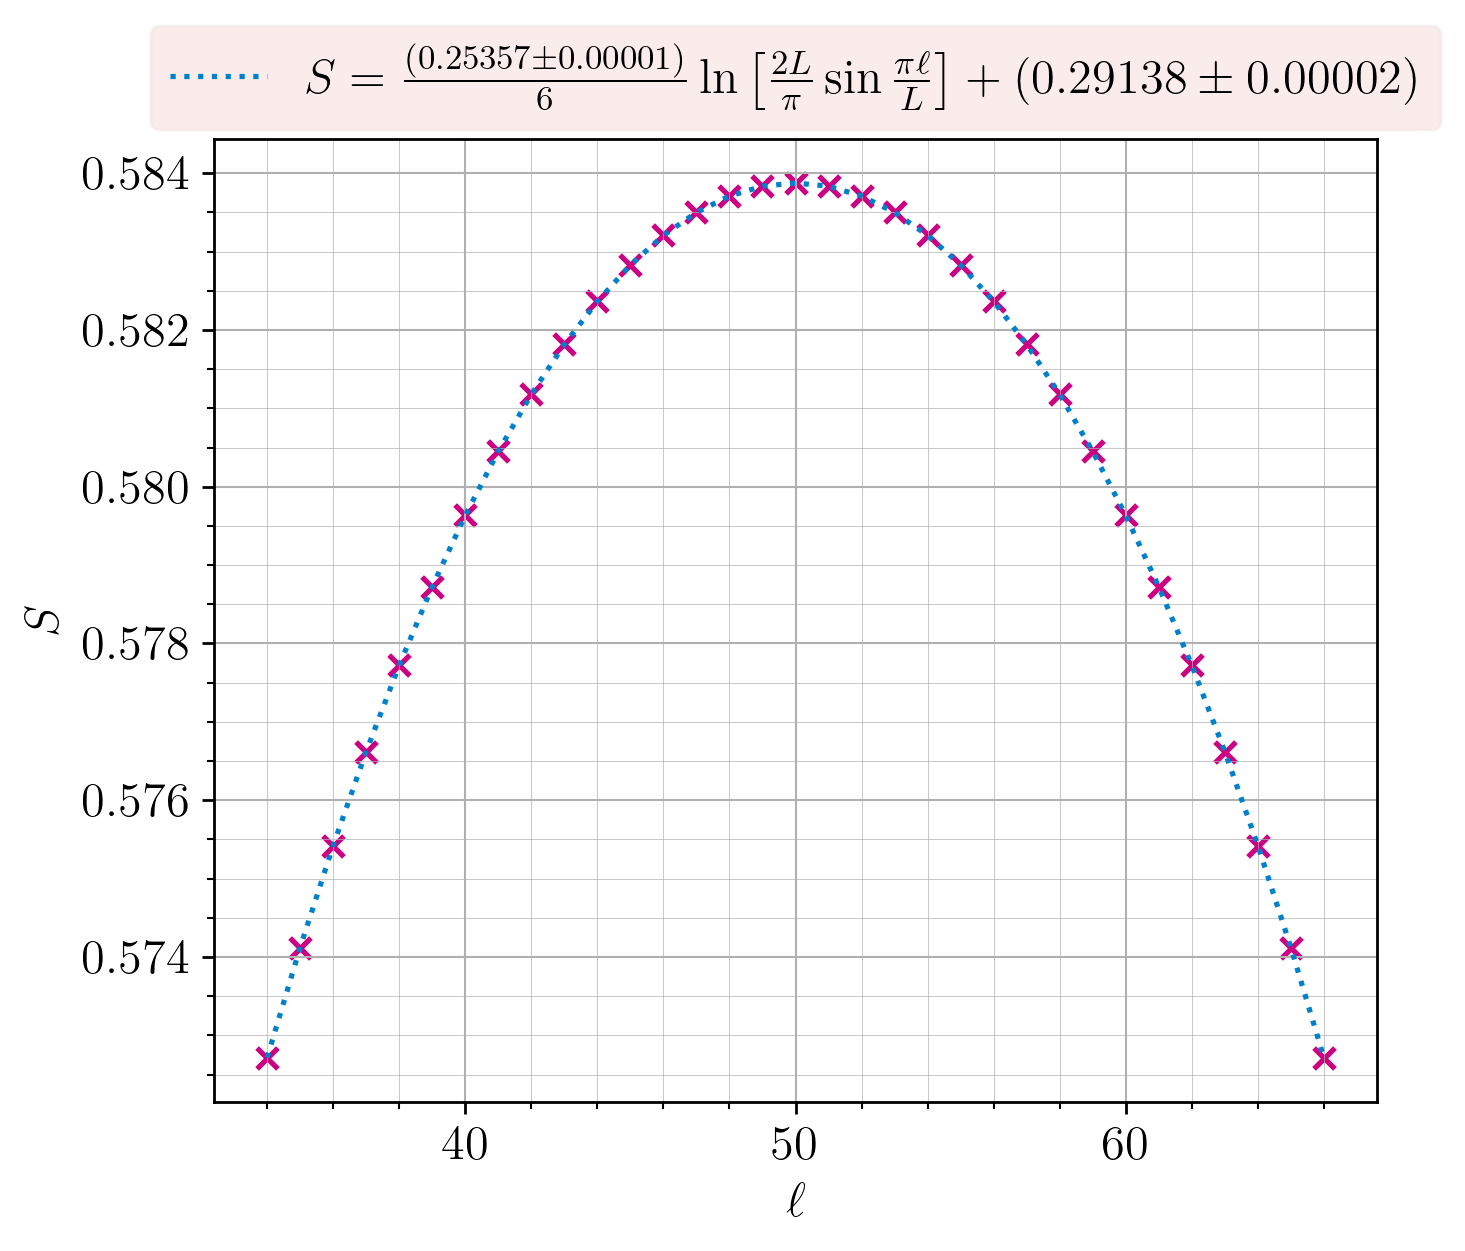
\includegraphics[scale=0.66]{../graphs/entropies/ff/alone_L=100.0_chi=100.0_J=1.0_h=1.0_i=1.0_3=0.0_c=0.0.png}\label{fig:cTFI.a}}\
		\subfloat[]{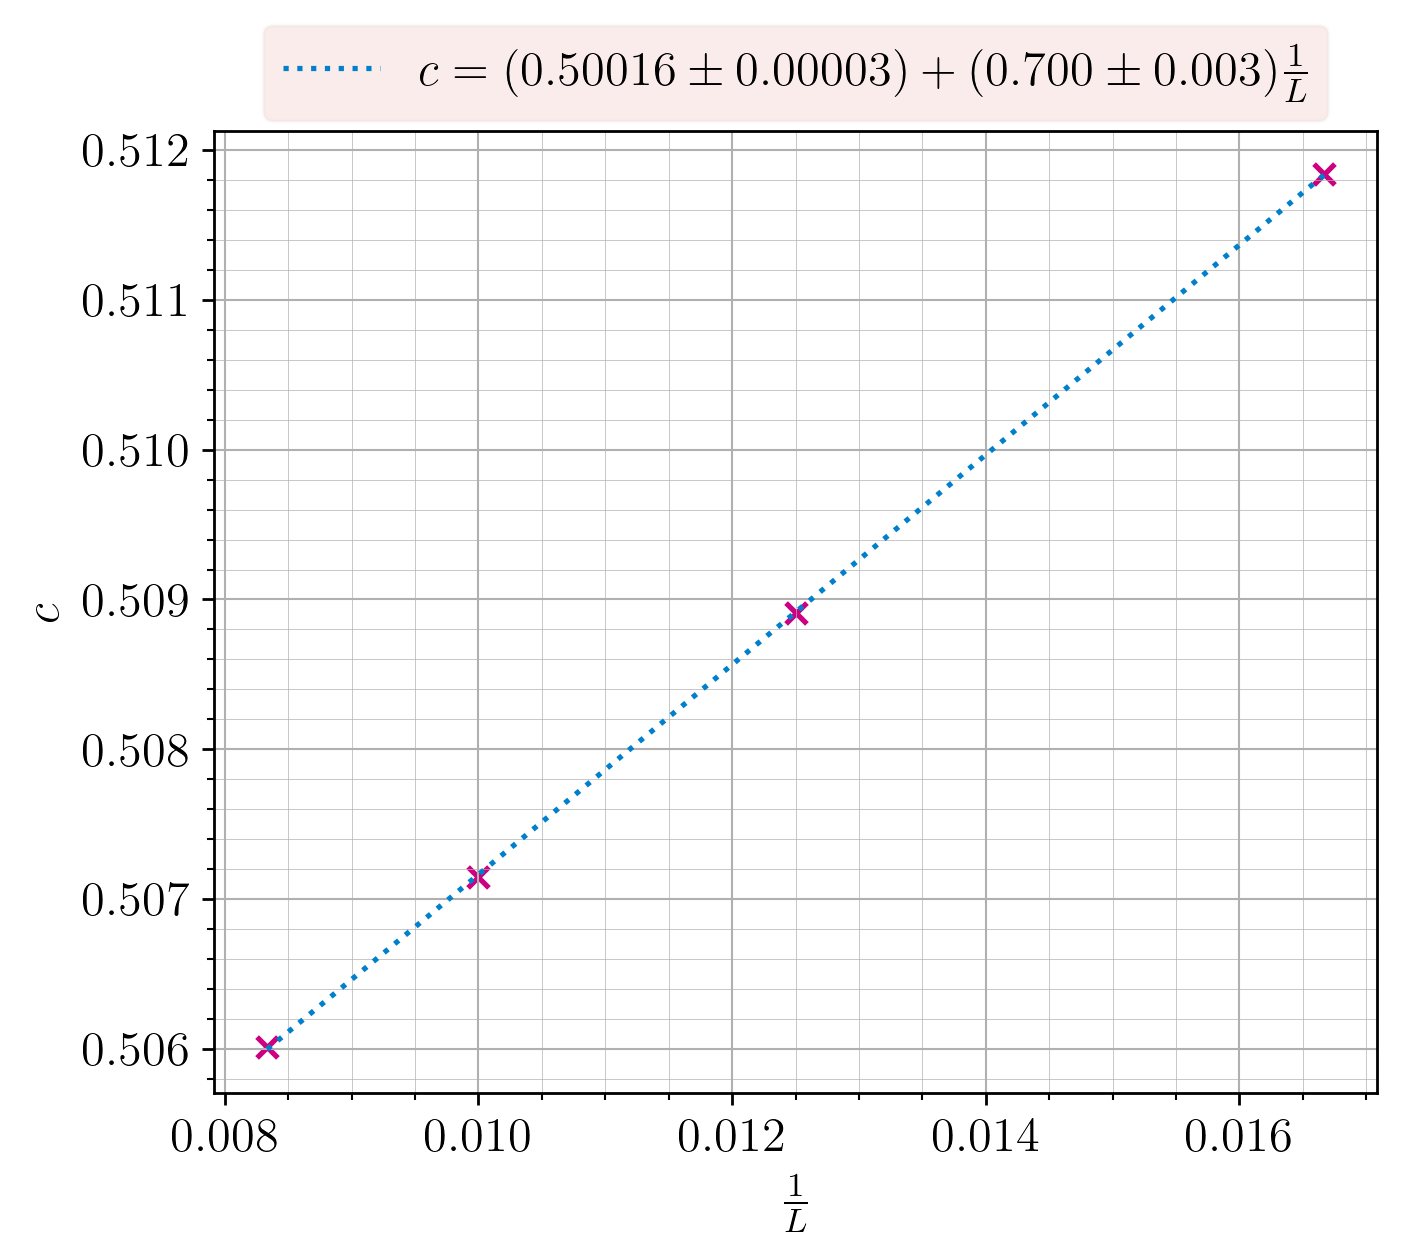
\includegraphics[scale=0.66]{../graphs/entropies/ff/calabrese_chi=100.0_J=1.0_h=1.0_i=1.0_3=0.0_c=0.0.png}\label{fig:cTFI.b}}
		\caption{Critical TFI with $\chi=100$ and $[ff]$ OBCs. (a): Typical fitting of the entanglement entropy with Cardy-Calabrese formula \eqref{eq:cardyOBCs} for $L=100$. (b): Extrapolation of the central charge.}
		\label{fig:cTFI}
	\end{figure}

	Noticing the expected value of central charge is obtained for critical TFI, it can be expected to obtain the correct central charge too for the OF model \eqref{eq:OF} for $\lambda_3/\lambda_I = 0.856$. According to \cite{obrien2018}, this point is described by TCI CFT, which has $c=7/10$. Therefore, \autoref{fig:cTCI} shows the results of the extrapolation of $c$ in $1/L$ for $[ff]$ OBCs. Both extrapolations with different formulas to recover $c$ for different lengths do not lead to the expected value, but slightly above $c\sim 0.77$. There can be several explanations for this to happen. At first, even if not shown, the bond dimension $\chi$ has no role at this point since the exact same extrapolated value of $c$ has been obtained for $\chi=200$, therefore this assumption that for the range of values for the bond dimension acceptable for normal computer does not play any role in results shown on \autoref{fig:cTCI}.

	\begin{figure}[h!]
		\hspace{-0.4cm}
		\subfloat[]{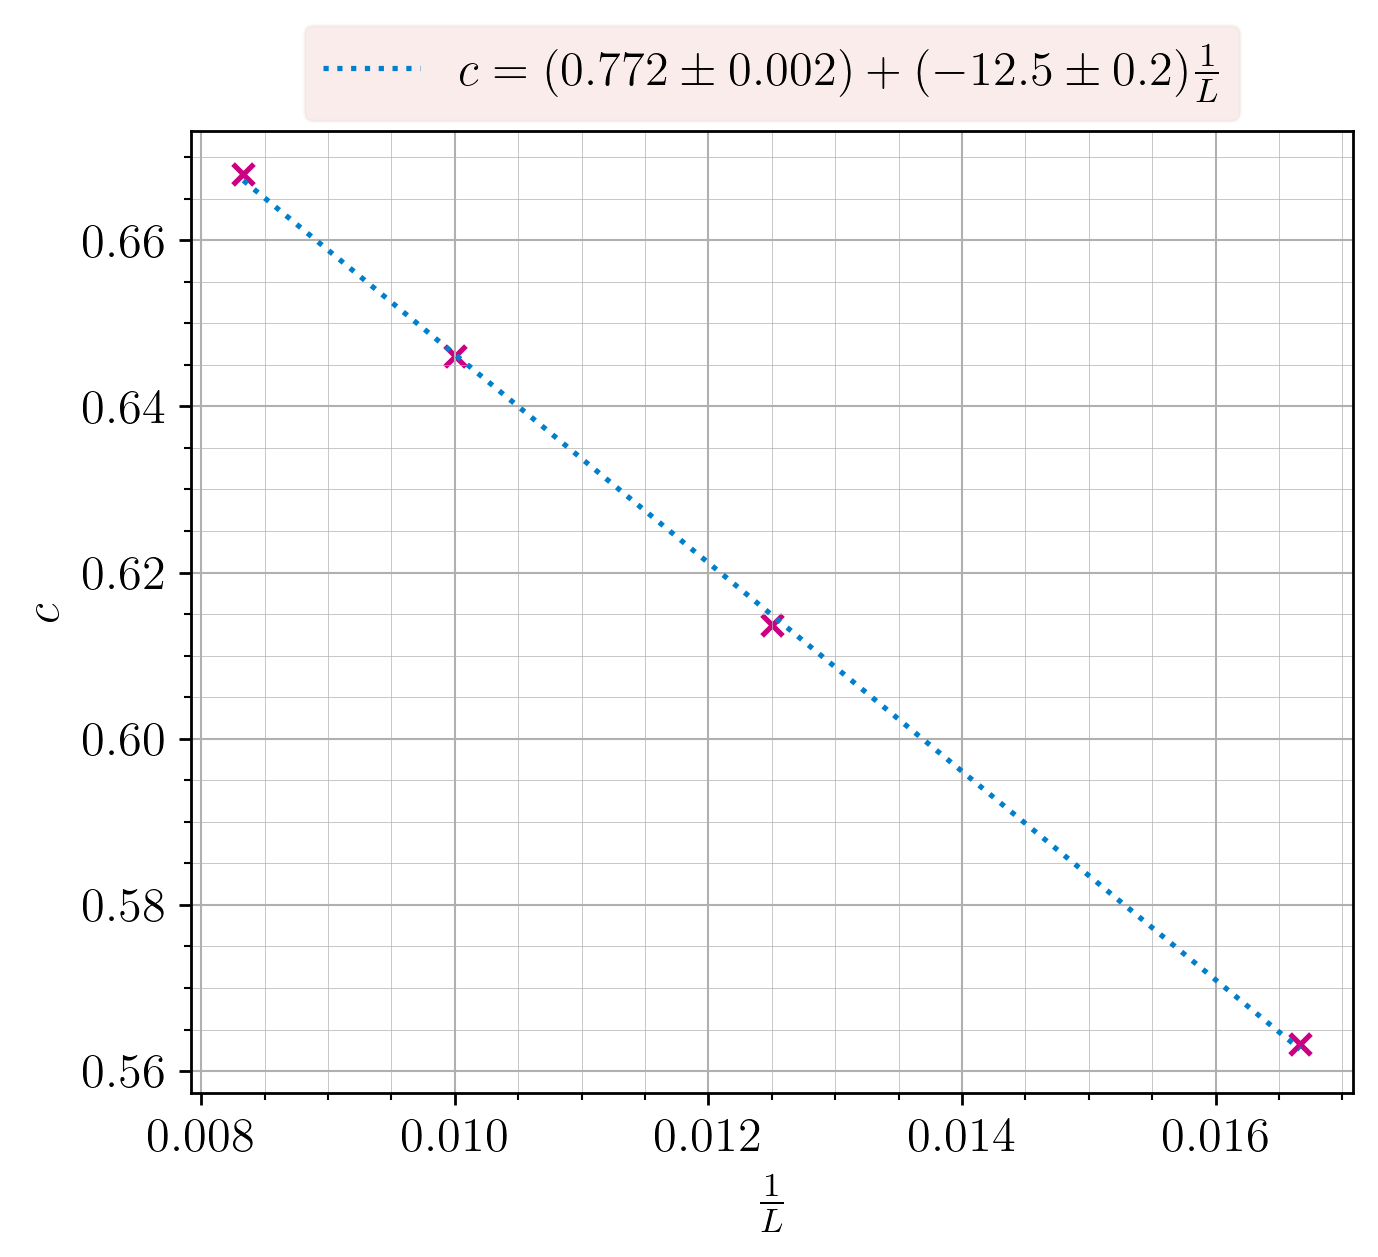
\includegraphics[scale=0.66]{../graphs/entropies/ff/calabrese_chi=100.0_J=1.0_h=1.0_i=1.0_3=0.856_c=0.0.png}\label{fig:cTCI.a}}\quad
		\subfloat[]{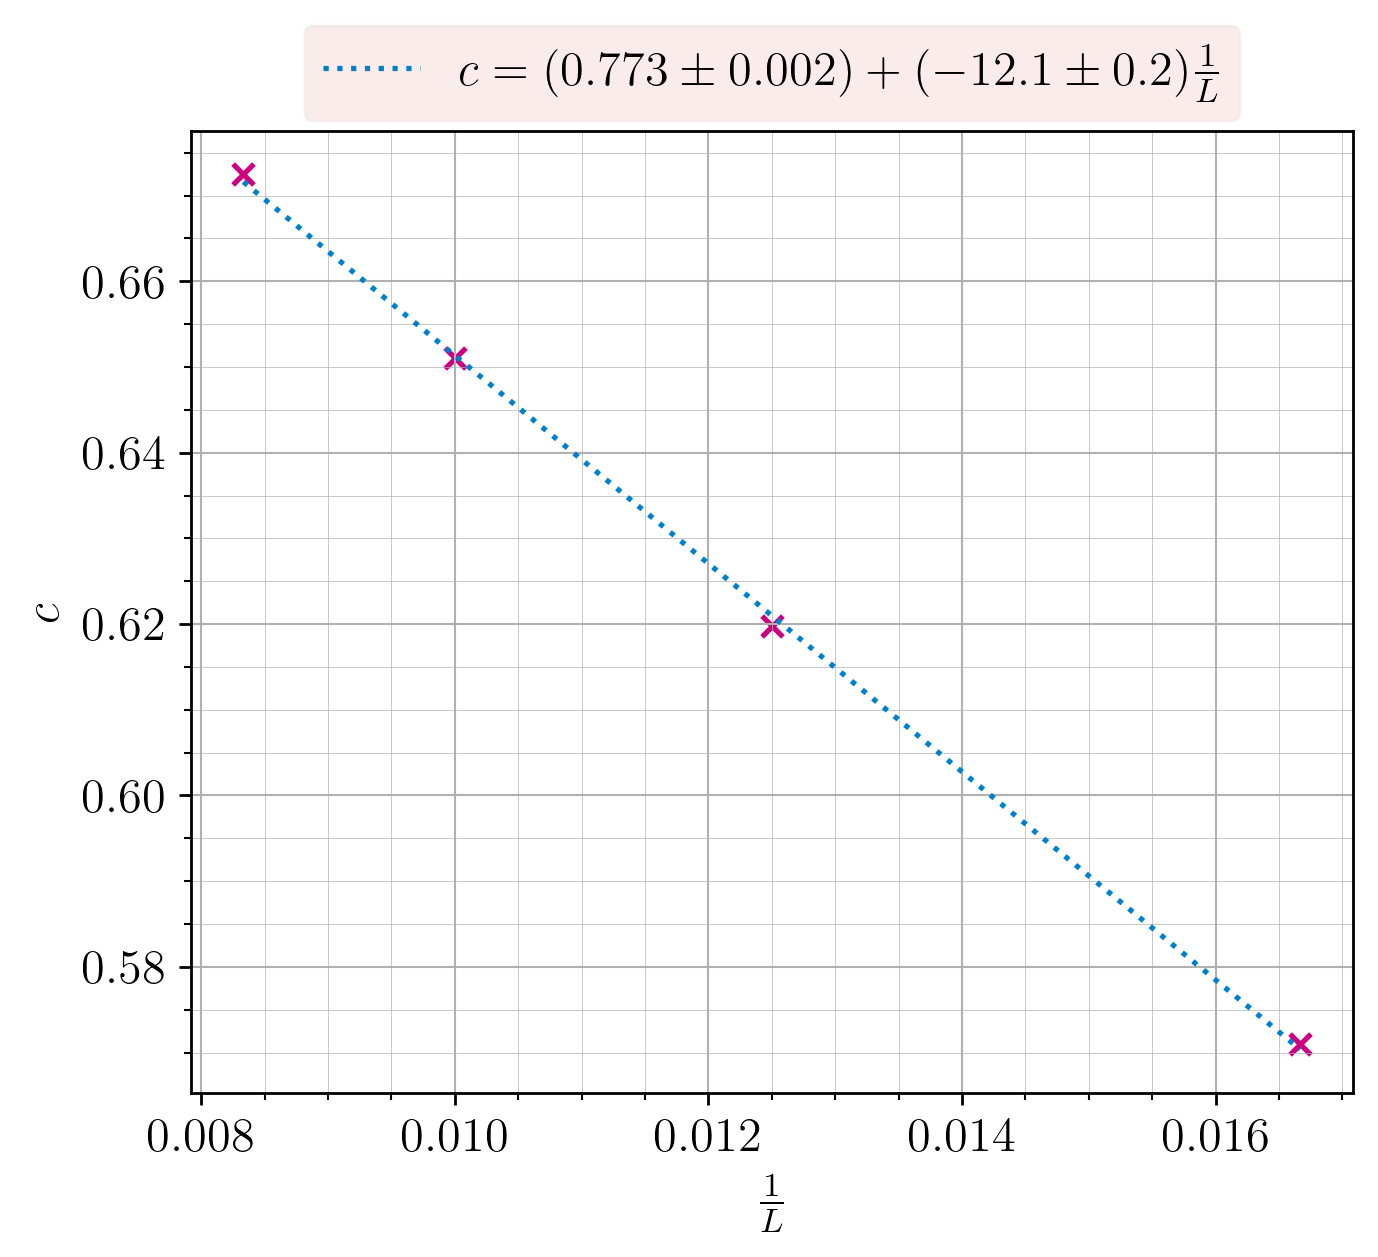
\includegraphics[scale=0.66]{../graphs/entropies/ff/other_chi=100.0_J=1.0_h=1.0_i=1.0_3=0.856_c=0.0.png}}
		\caption{Extrapolation of the central charge for $\lambda_3/\lambda_I=0.856$, $\chi=100$ and $[ff]$ OBCs (a): with Cardy-Calabrese formula \eqref{eq:cardyOBCs}. (b): with \eqref{eq:otherOBCs}.}
		\label{fig:cTCI}
	\end{figure}

	Hence, it can be useful to look at how the extrapolations of $c$ behave for different values of $\lambda_3/\lambda_I$, as in \autoref{fig:phaseOBCs}, for $[ff]$ OBCs. It is expected that $c =1/2$ for values $\lambda_3/\lambda_I \in [0, 0.856[$, $c=7/10$ for $\lambda_3/\lambda_I =0.856$ and $c=0$ for $\lambda_3/\lambda_I>0.856$ \cite{obrien2018}. The observation of the figure then tells a few things. For $0\leq \lambda_3/\lambda_I \leq 0.6$ the central charge follows a straight line in $1/L$ converging to $c\sim 0.5$ even though the linearity seems broken for small lengths for $\lambda_3/\lambda_I=0.6$. However, even if for $0.7\leq \lambda_3/\lambda_I \leq 0.82$ the convergence to $c\sim 0.5$ appears to still be present, the central charge passes through a maximum at a finite length, that has been checked to correspond to the moment the correlation length computed at the middle of the chain becomes equal to the length $L$ of the chain. % maybe expalain correlation length
	This behavior seems to be found again for $0.83\leq \lambda_3/\lambda_I \leq 0.85$ except that the length for which $c$ was computed are not large enough to observe a maximum but it can be inferred that it would appear for larger lengths. However, there is nothing compelling to say they must converge to $c\sim 0.5$. For $\lambda_3/\lambda_I=0.856$, the behavior found in \autoref{fig:cTCI.a} is repeated and the convergence to $c\sim 0.77$ also is. Finally, for $\lambda_3/\lambda_I=0.86$, a maximum is again reached but this time it can be expected that $c$ goes to $0$ for larger lengths, even though no conclusions can made. Overall, the \autoref{fig:phaseOBCs} shows that the behavior of $c$ in $1/L$ is incorrect, partially unexpected and no clear conclusion can be drawn. This can explain the incorrect value of the central charge in the TCI point found in \cite{obrien2018}.

	\begin{figure}[h!]
		\centering
		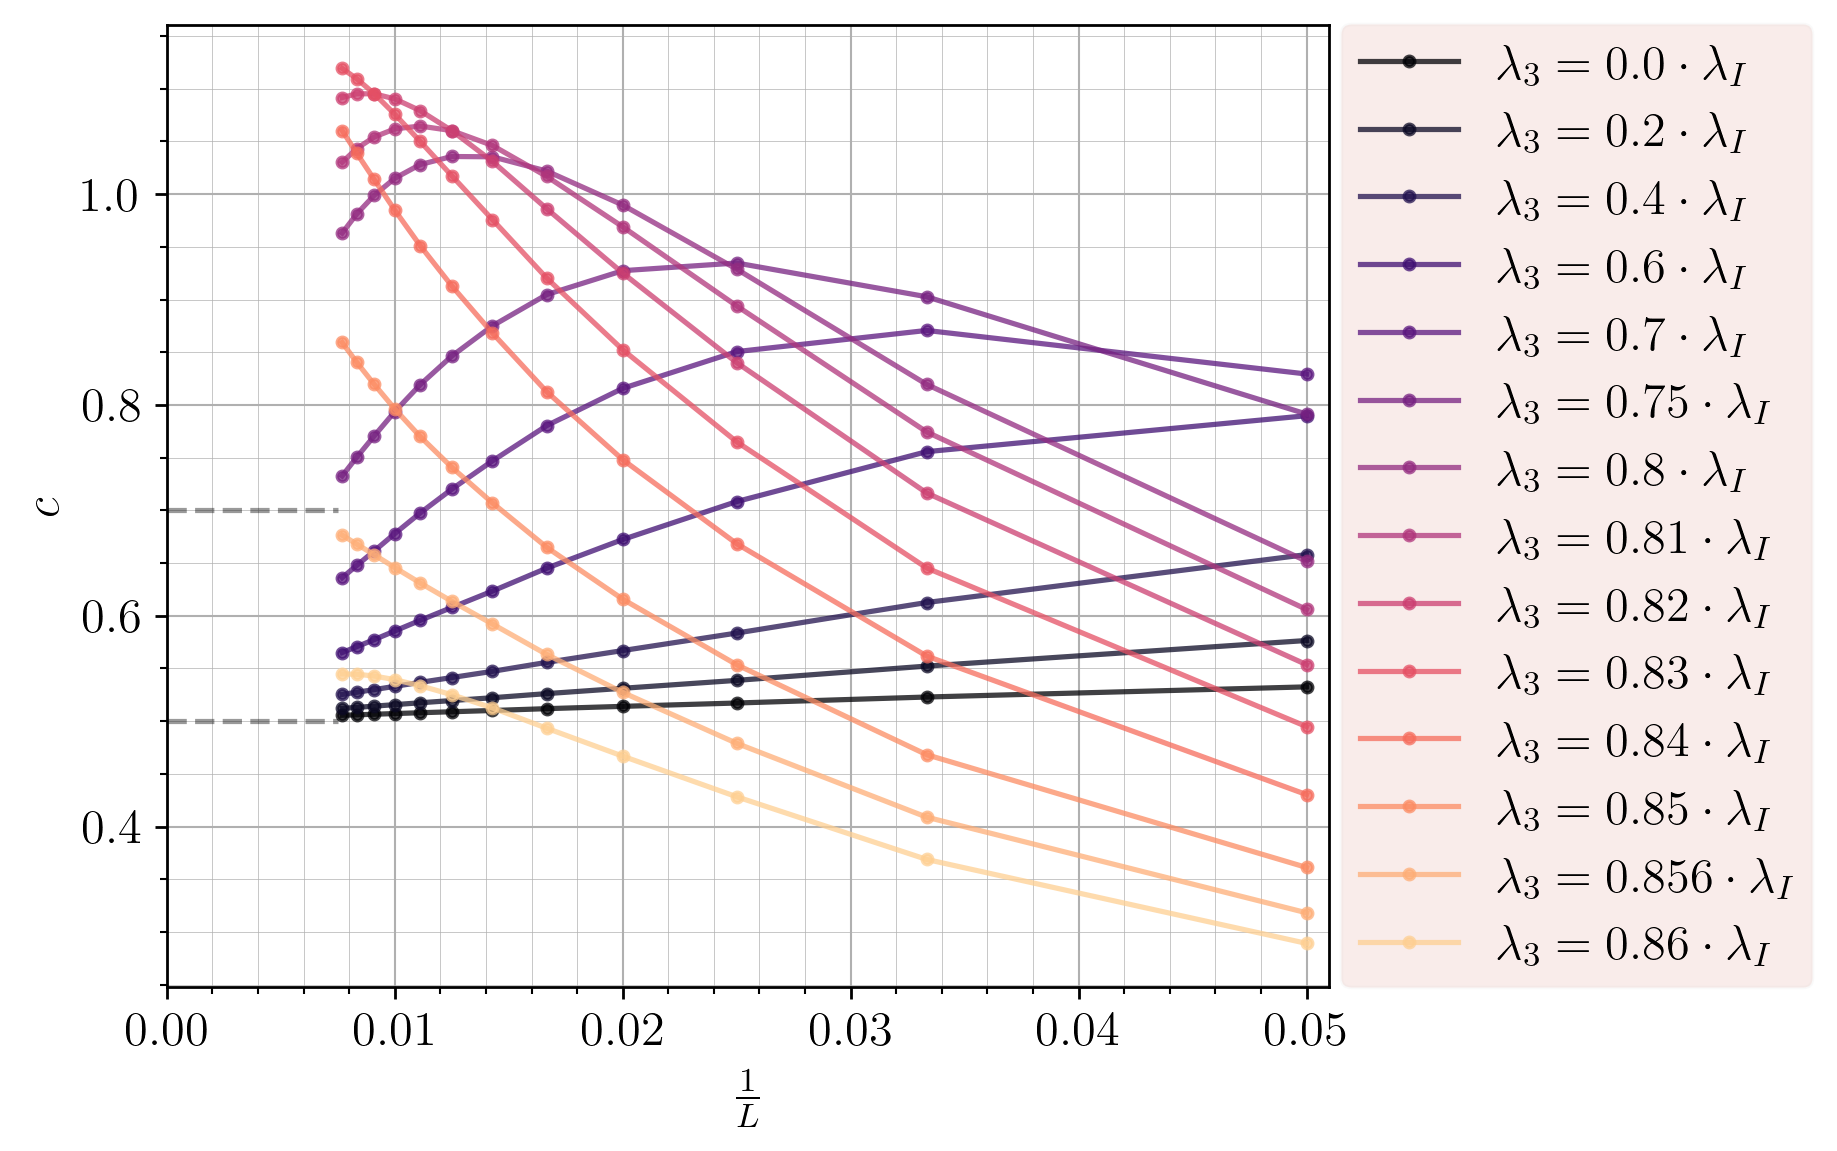
\includegraphics[scale=0.66]{../graphs/phase/ff/chi=100.0_J=1.0_h=1.0_i=1.0_c=0.0.png}
		\caption{Extrapolation of the central charge with Cardy-Calabrese formula \eqref{eq:cardyOBCs} as $\lambda_3/\lambda_I$ is varied with $\chi=100$ and $[ff]$ OBCs. Dashed grey lines are added as guides for $c=1/2$ and $7/10$.}
		\label{fig:phaseOBCs}
	\end{figure}

	The central charge reaching a maximum can be due to extra entanglement throughout the chain, coming from the edge states. % cite if possible
	To try to remove them, to pin the edge spins with on-site magnetic field can be efficient. 

	To find an adequate value of the pinning field for different boundary conditions presented on \autoref{tab:pinningBCs}, the spin expectation values at both boundary sites can be computed by changing the pinning field magnitude $h_\text{pin}$ in the $x$-direction. This is shown on \autoref{fig:edgesSpin} for $\lambda_3/\lambda_I=0.856$ and $L=30$. It can be noticed that the spins are totally aligned to the magnetic field for $|h_\text{pin}|>20$. To be certain of this, the value of $|h_\text{pin}|=100$ will be taken from now on. It can also be observed that the $[ff]$ OBCs let the edges spin alone with $\ev{\sigma^x_l}=0$, however for $[f-]$ OBCs the free edge acquires a small $\ev{\sigma^x_l}\sim -0.1$. It will be seen later on that this seems to not be problematic. It is worth mentioning moreover that \autoref{fig:edgesSpin} has been checked to neither be specific to the model used nor the length of the chain.

	\begin{figure}[h!]
		\centering
		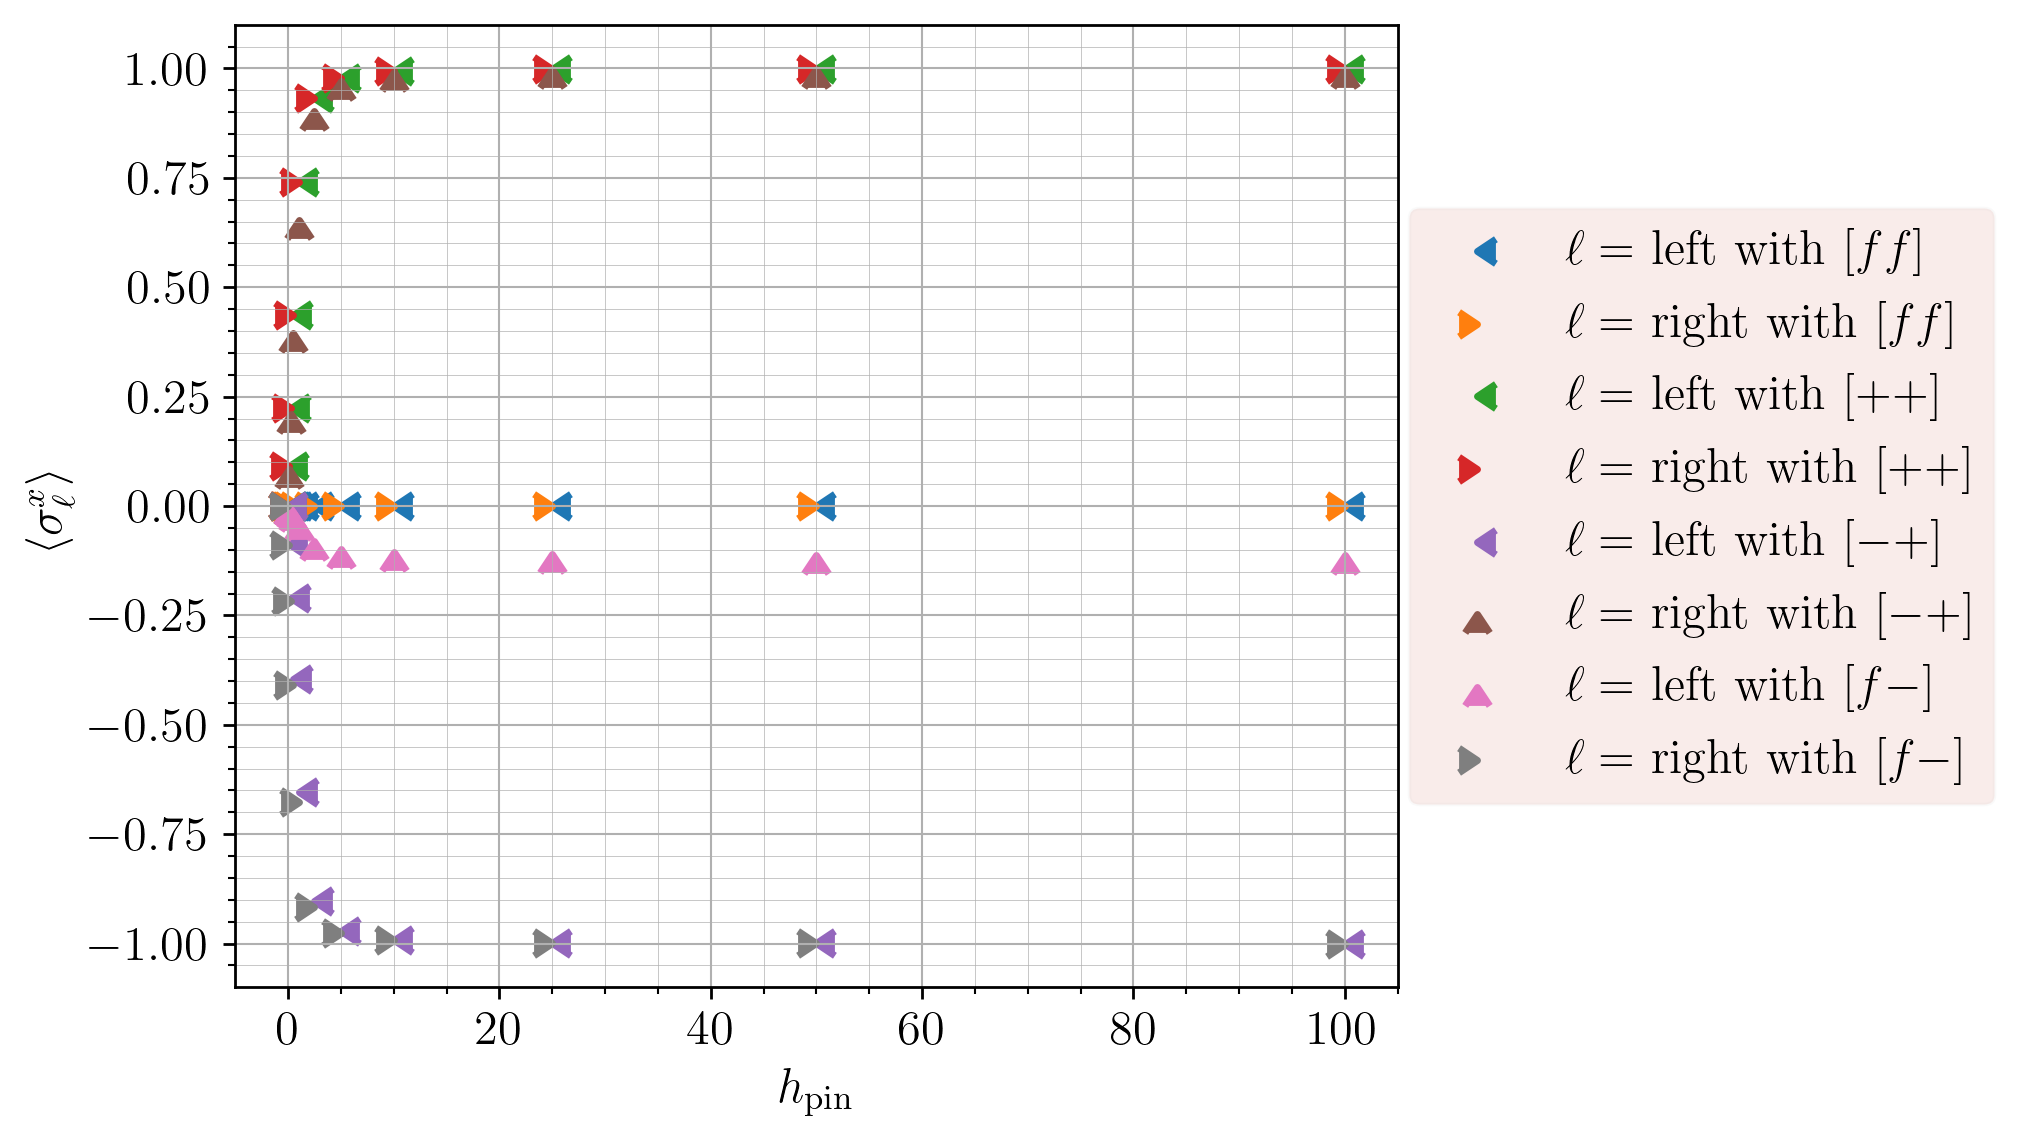
\includegraphics[scale=0.66]{../graphs/edge/L=30.0_chi=50.0_J=1.0_h=1.0_i=1.0_3=0.856_c=0.0.png}
		\caption{Spin at the edges of the chain while pinning them with various $h_\text{pin}$ magnitudes and under different OBCs for $L=30$, $\chi=50$ and $\lambda_3/\lambda_I=0.856$.}
		\label{fig:edgesSpin}
	\end{figure}

	To confirm that the pinning field does not break the behavior of the spins in the bulk, the spin expectation value in the middle of the chain is computed for multiple values of $h$ for TFI \eqref{eq:TFI} and different OBCs for $L=30$. The behavior is the exact one expected \cite{yang1951, pfeuty1970} through the transition at $J=h$ as seen in \autoref{fig:spinTFI}, with the $\langle \sigma^x_{L/2}\rangle$ having the correct sign in the ordered phase $h<J$ forced by the pinning field at the edges. Moreover, the behavior of the $\langle \sigma^x_{L/2}\rangle$ is fully expected \cite{pfeuty1970}. Therefore, the pinning of the edge spins seems to imply a correct behavior of the system at least for the TFI model.

	\begin{figure}[h!]
		\hspace{-0.4cm}
		\subfloat[]{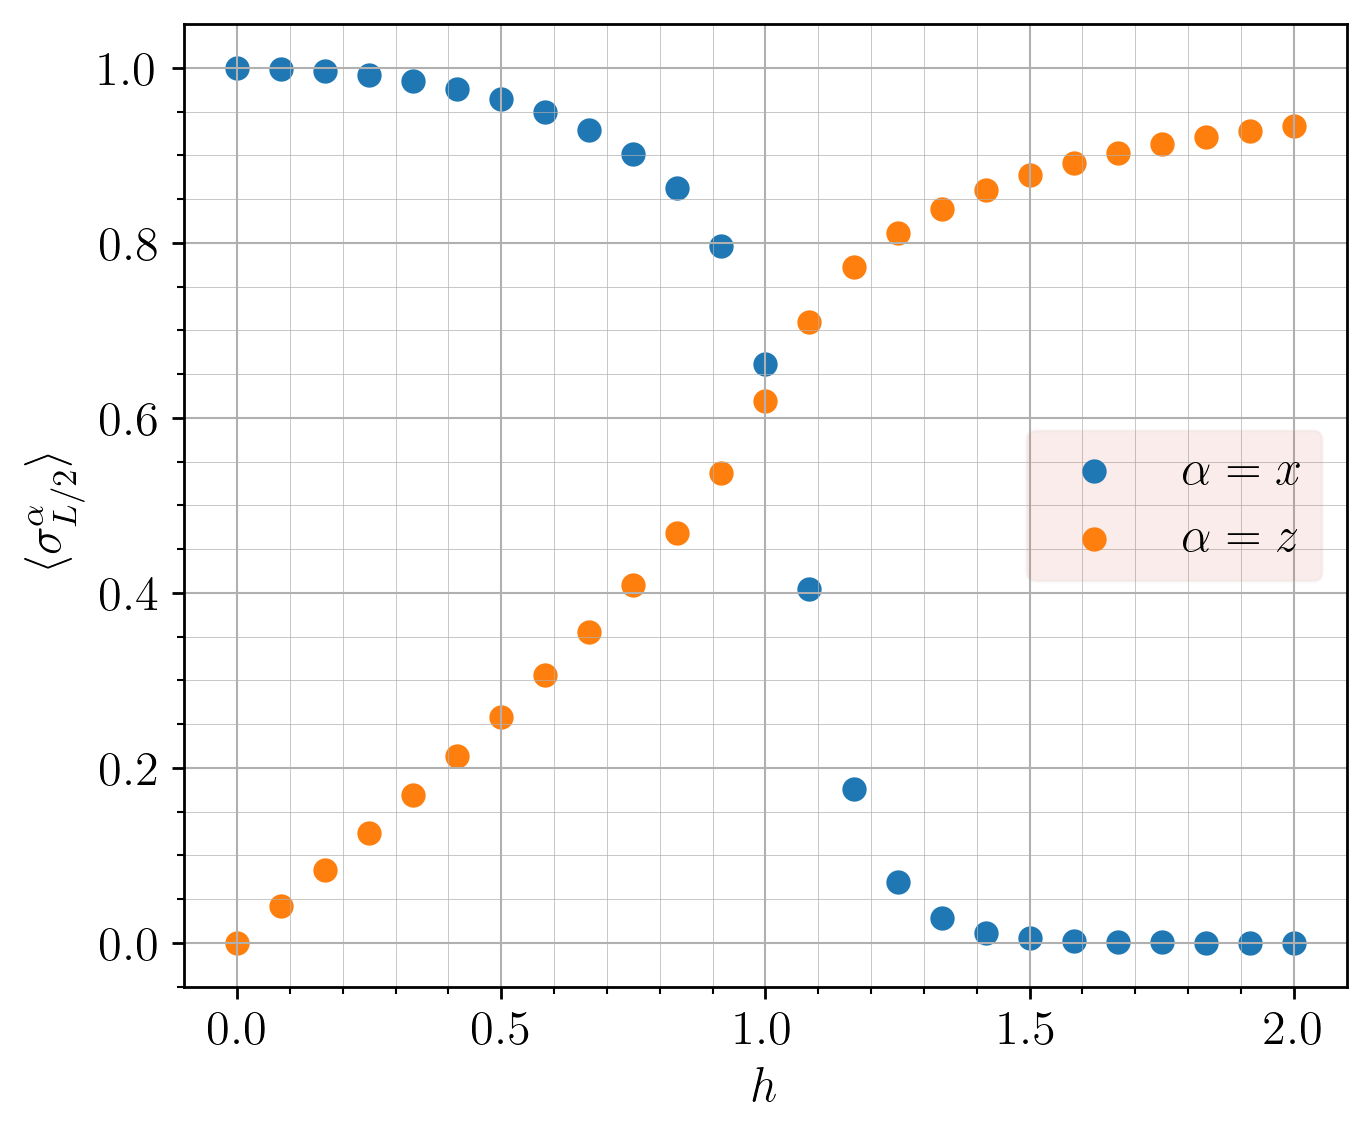
\includegraphics[scale=0.66]{../graphs/spin/--/100/L=30_chi=30.0_J=1.0_i=1.0_3=0.0_c=0.0.png}}\quad
		\subfloat[]{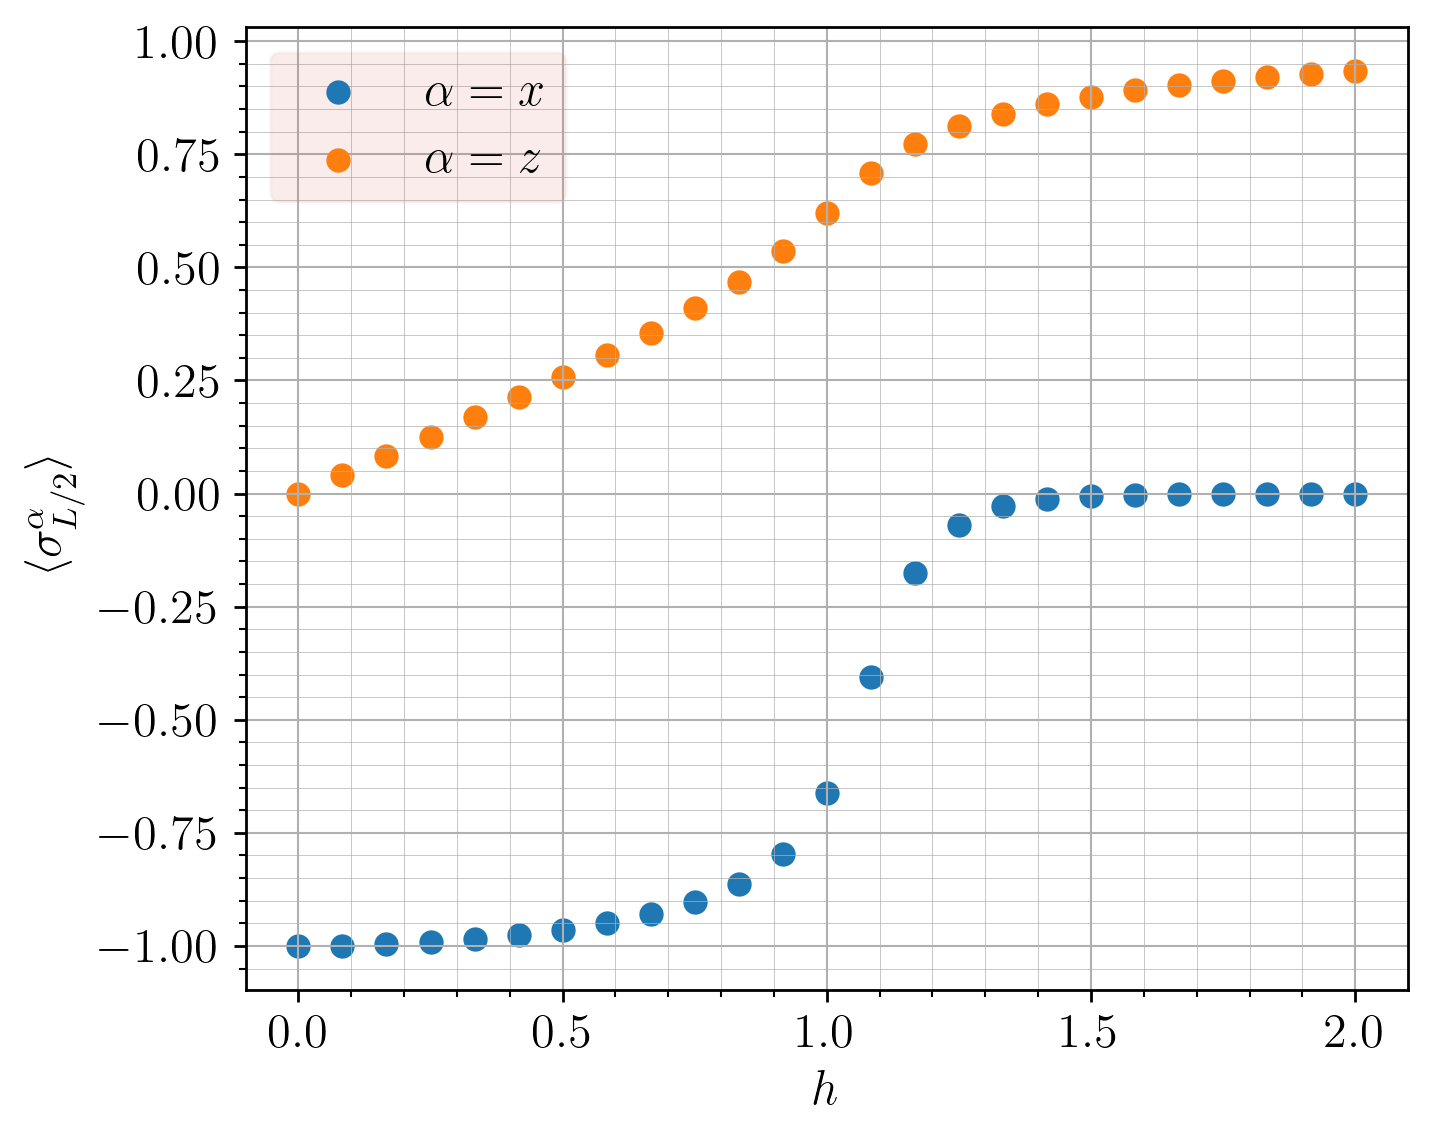
\includegraphics[scale=0.66]{../graphs/spin/++/100/L=30_chi=30.0_J=1.0_i=1.0_3=0.0_c=0.0.png}}
		\caption{Spin expectation values of TFI with $J=1$ in the middle of the chain for $L=30$ and $\chi=30$ (a): with $[++]$ OBCs and $h_\text{pin}=-100$. (b): with $[--]$ OBCs and $h_\text{pin}=100$.}
		\label{fig:spinTFI}
	\end{figure}

	To confirm further and try to find the correct value $c=7/10$ of the TCI CFT point $\lambda_3/\lambda_I=0.856$, the central charge is extrapolated for $[++]$ OBCs with $h_\text{pin}=100$. For critical TFI, the central charge is correctly recovered as $c=0.50029\pm 0.00008$ in the large $L$ limit. It can be noted that the slope in now negative as compared to the one on \autoref{fig:cTFI.b} where it is positive. This can from the reduce in entanglement entropy from pinning the edge spins. On the other hand, the result obtained for $\lambda_3/\lambda_I=0.856$ is $c= 0.594\pm 0.002$ which is even worse than the one obtained with $[ff]$ OBCs in \autoref{fig:cTCI.a} being $c=0.772 \pm 0.002$. The linearity seems to be slightly off this time even if still acceptable with $R^2=0.999$, but it exhibits the fact that this pinning has strongly affect the system and the linear regression might no be correct, at least for such small lengths.

	\begin{figure}[h!]
		\hspace{-0.4cm}
		\subfloat[]{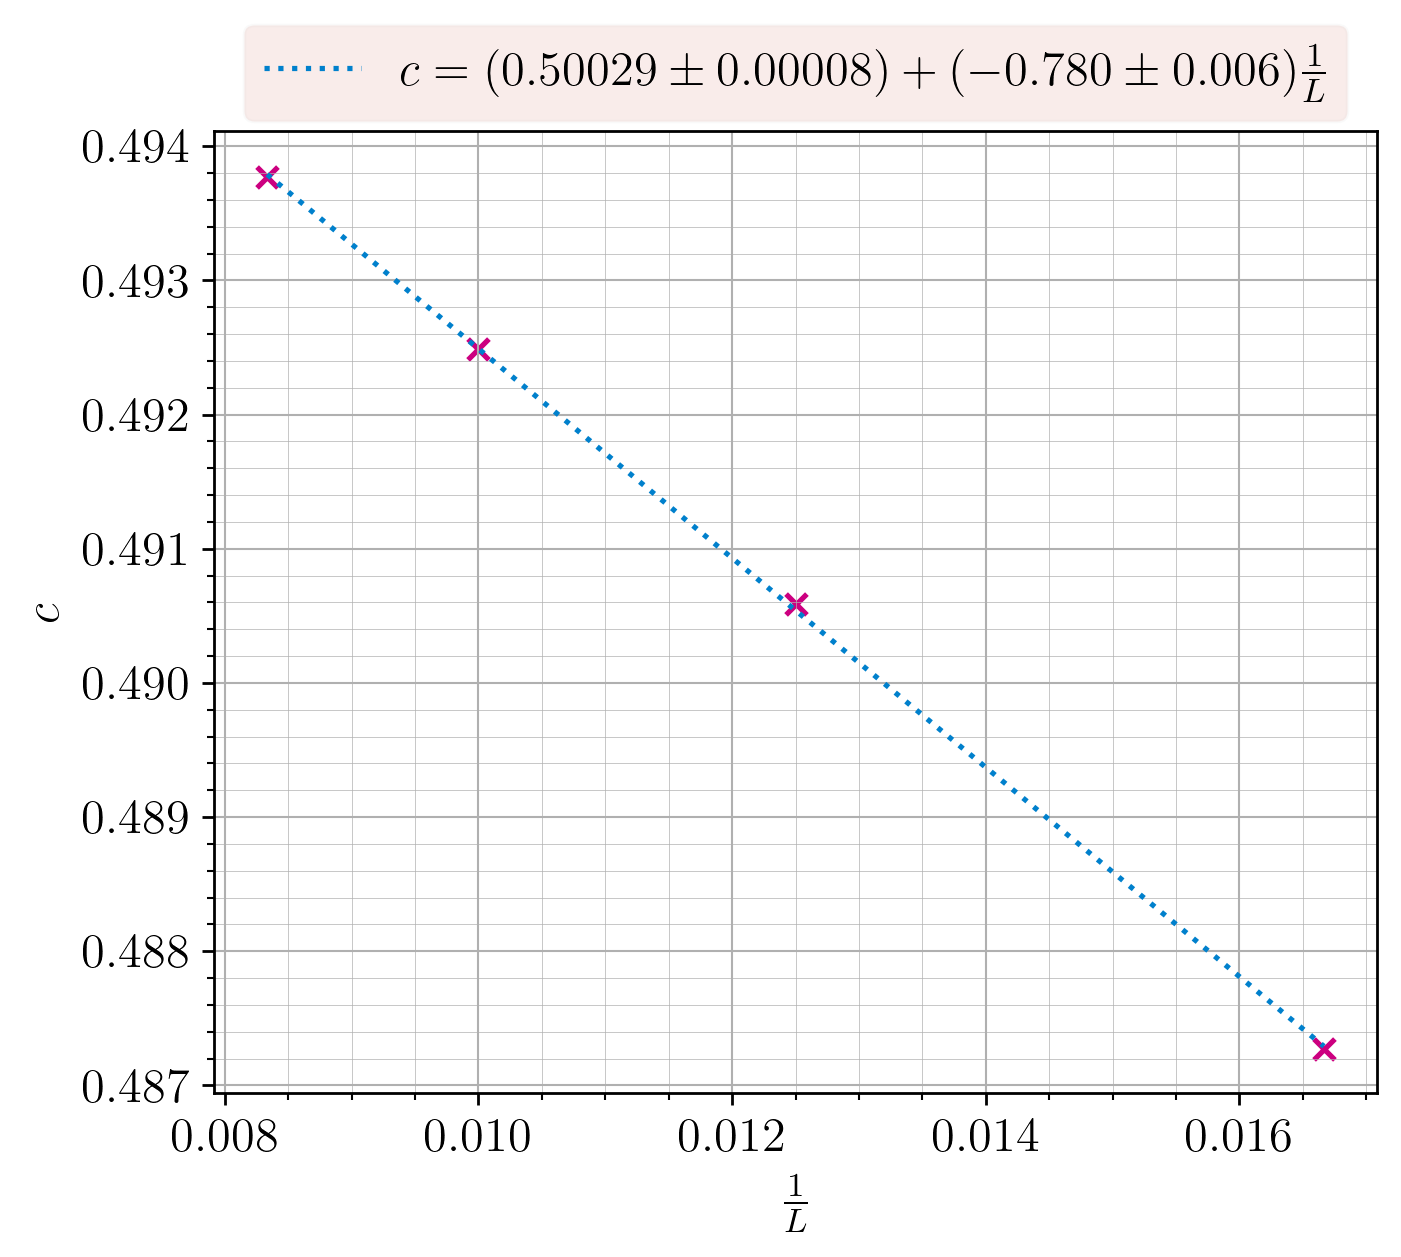
\includegraphics[scale=0.66]{../graphs/entropies/--/100/calabrese_chi=100.0_J=1.0_h=1.0_i=1.0_3=0.0_c=0.0.png}}\quad
		\subfloat[]{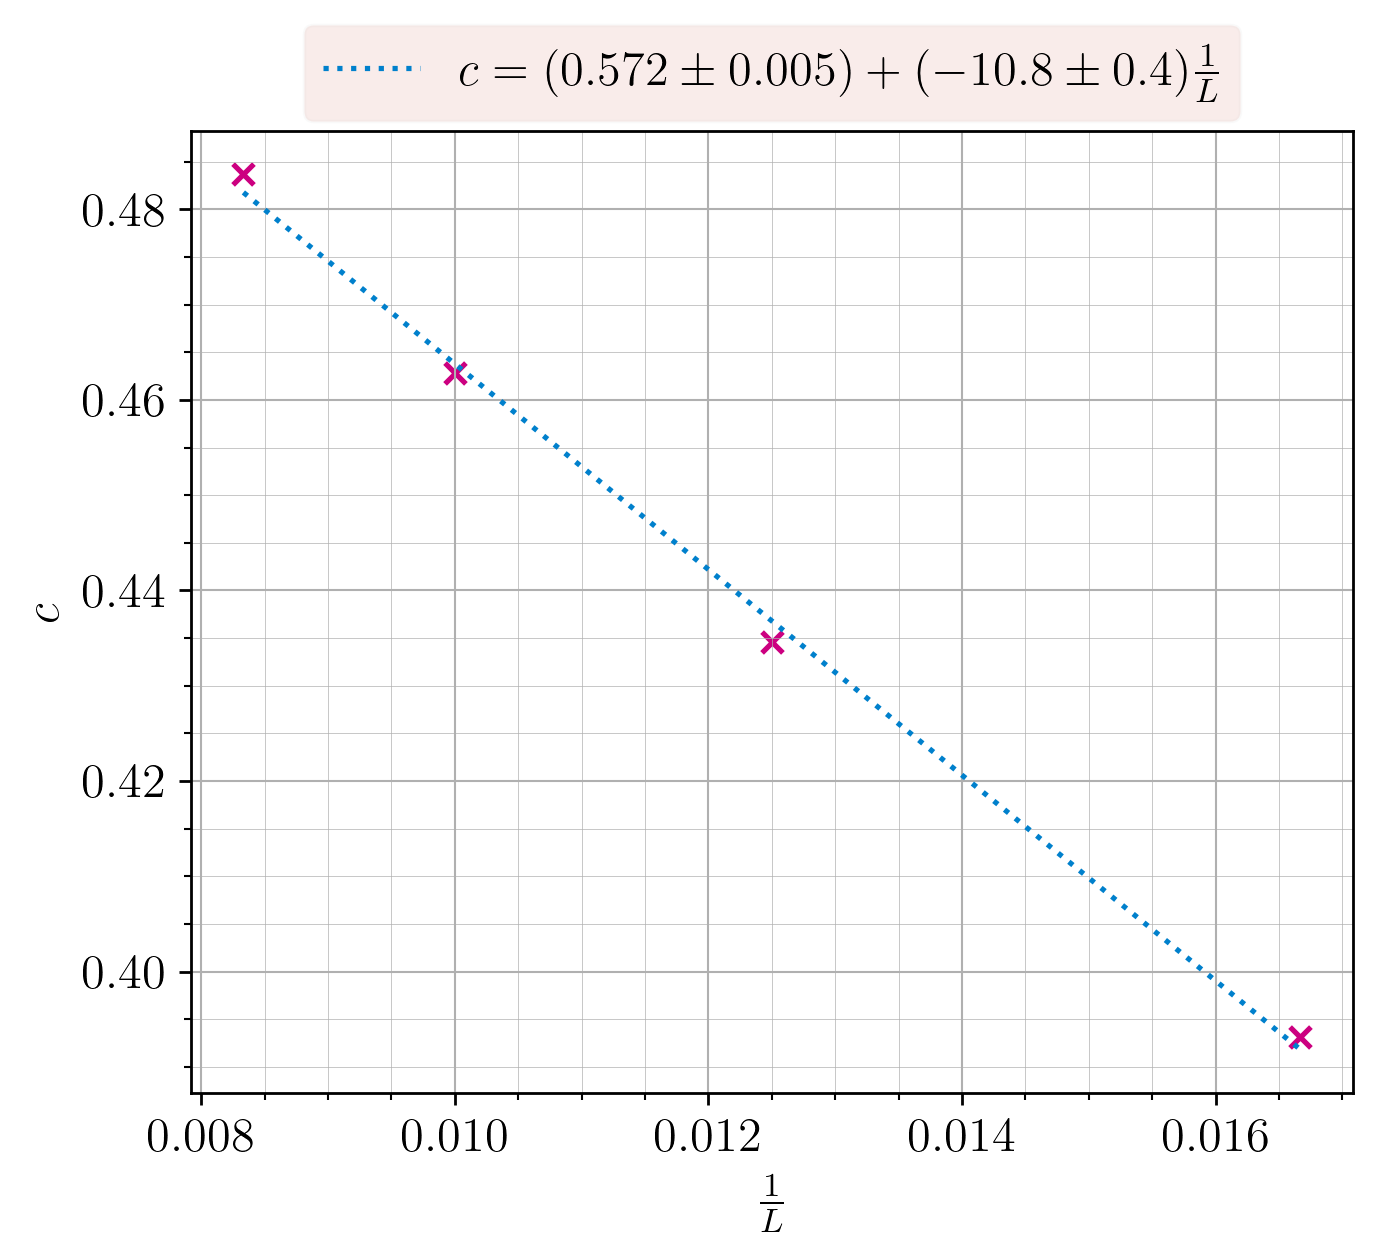
\includegraphics[scale=0.66]{../graphs/entropies/--/100/calabrese_chi=100.0_J=1.0_h=1.0_i=1.0_3=0.856_c=0.0.png}}
		\caption{Extrapolation of the central charge with Cardy-Calabrese formula for $[++]$ OBCs with $h_\text{pin}=-100$ (a): for critical TFI and $\chi=100$. (b): for $\lambda_3/\lambda_I = 0.856$ and $\chi$ sufficiently large to have ground state variance $\sim 10^{-9}$.}
		\label{fig:cPin}
	\end{figure}

	Therefore, another procedure that can be followed to characterize the $\lambda_3/\lambda_I = 0.856$ point is to build conformal towers expected from the CFT describing the corresponding critical point, as well as the ground state energy scaling. To do so, the excitation energies must be retrieved. Following the procedure of \cite{chepiga2017}, the typical behavior of the $10$ first energies found for critical TFI for length $L=70$ is presented on \autoref{fig:energiesTFI} for one complete sweep. It is worth noticing that the Hamiltonian \eqref{eq:TFI} has been rescaled to $\mc H \to \mc H/4$ so that is it now expressed in terms of spin matrices $S^\alpha = \sigma^\alpha/2$. The energies reach a minimum in the middle of the chain, except for the ground state energy, and this value in perfected throughout the sweeps. This minimum will be taken as the value of the excitation energy, again following the work done in \cite{chepiga2017}.

	\begin{figure}[h!]
		\centering
		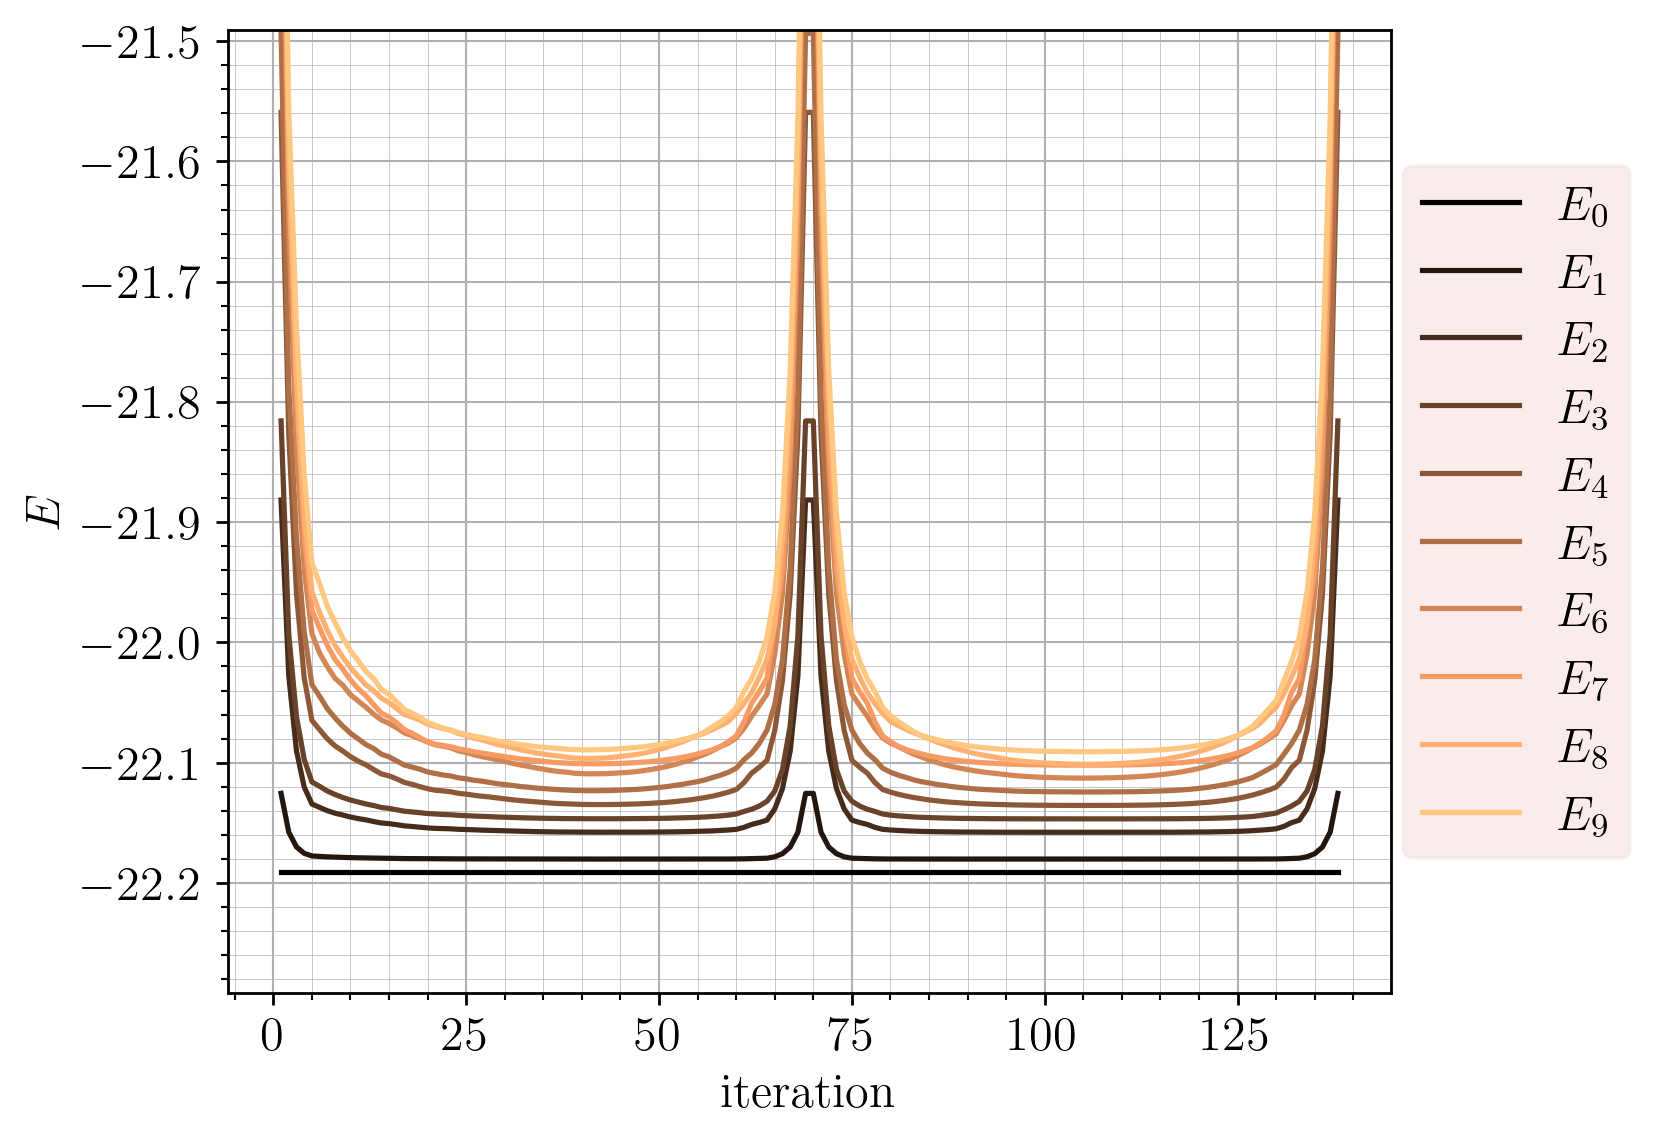
\includegraphics[scale=0.66]{../graphs/conformal/ff/energies_L=70.0_chi=50.0_J=0.25_h=0.25_i=0.5_3=0.0_c=0.0.png}
		\caption{Typical behavior of the lowest-lying energies for one converging sweep of TFI at criticality $J=h$ for one sweep with $L=70$, $\chi=50$ and $[ff]$ OBCs.}
		\label{fig:energiesTFI}
	\end{figure}

	To confirm the correctness of the excited energies $E_n$ -- at least the two first -- the gap of TFI for different values of $h$ is computed and shown on \autoref{fig:gapsTFI} for $L=50$ as well as the extrapolation of the gap in the thermodynamic limit. For $h<J$ the system is ferromagnetic and breaks the $\mathbb Z_2$-symmetry, therefore two degenerate ground states $\ket{+\cdots +}$ and $\ket{-\cdots -}$ are present and thus $|E_1- E_0|$ is expected to vanish. The gap in this ordered phase is expected to be $2|J|(1-|h|)$ \cite{pfeuty1970} and is exactly the value found for $|E_2-E_0|$, knowing that $J=1$ here. Moreover, for $h>J$ the systems is paramagnetic and has a non-degenerate ground state with a gap $2|J|(|h|-1)$. Finally, for $J=h$, the systems goes under a phase transition and expected to have a continuous spectrum. The gap is then observed to close exponentially fast in $1/L$.

	\begin{figure}[h!]
		\hspace{-0.5cm}
		\subfloat[]{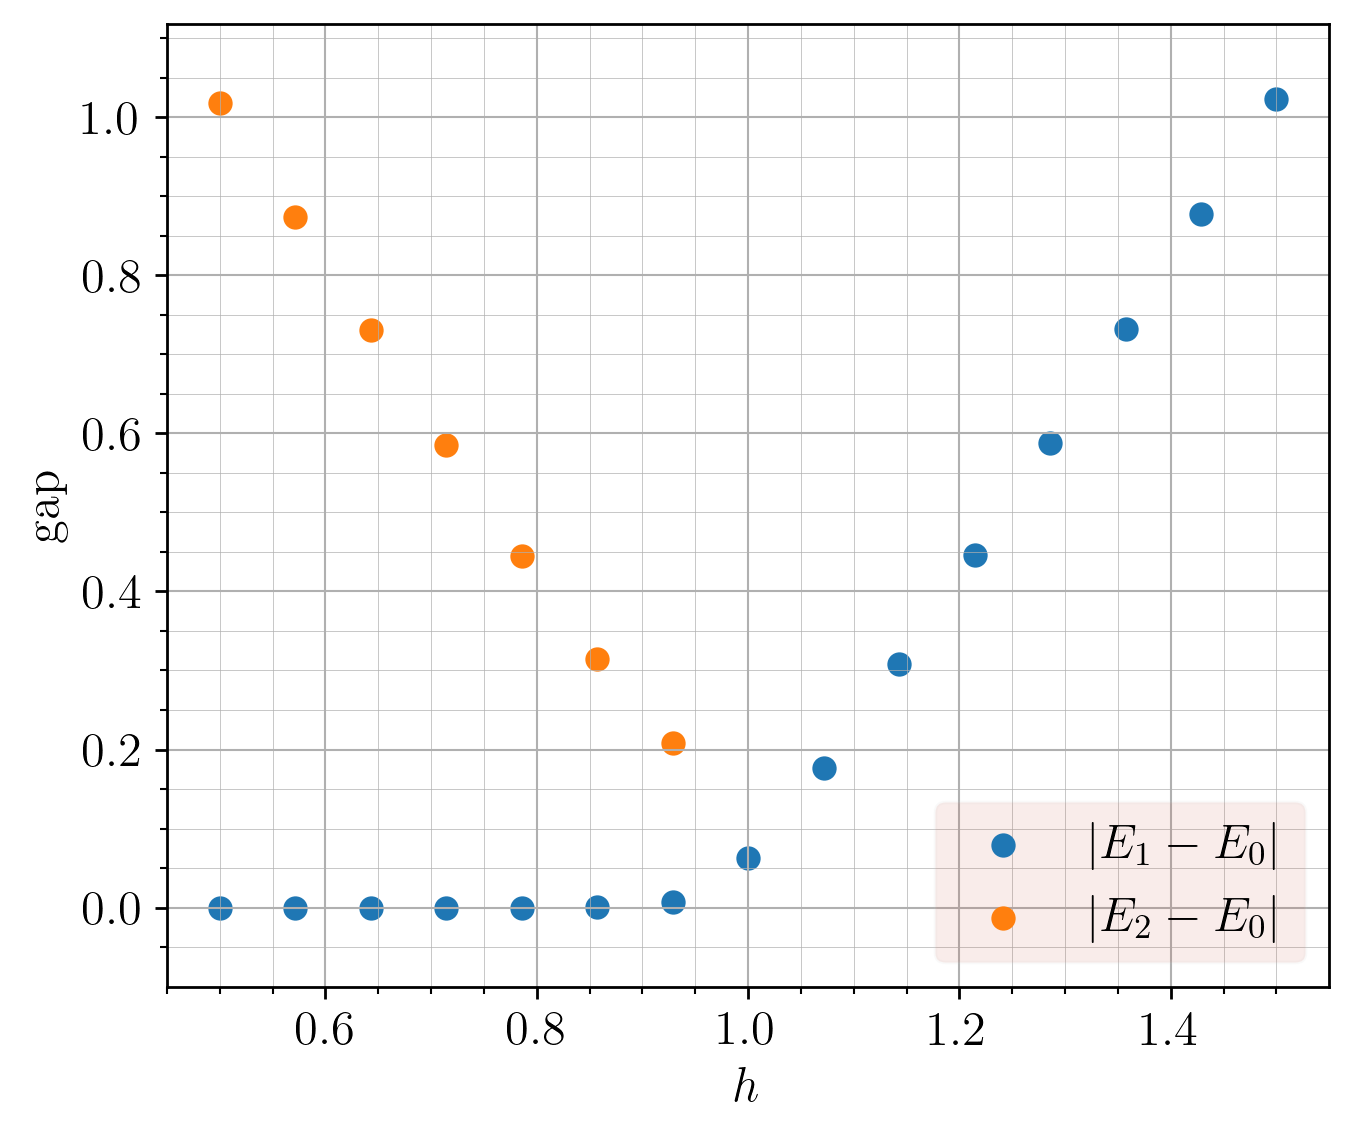
\includegraphics[scale=0.66]{../graphs/transition/ff/gap_L=50_chi=50.0_J=1.0_i=0.5_3=0.0_c=0.0.png}}\quad
		\subfloat[]{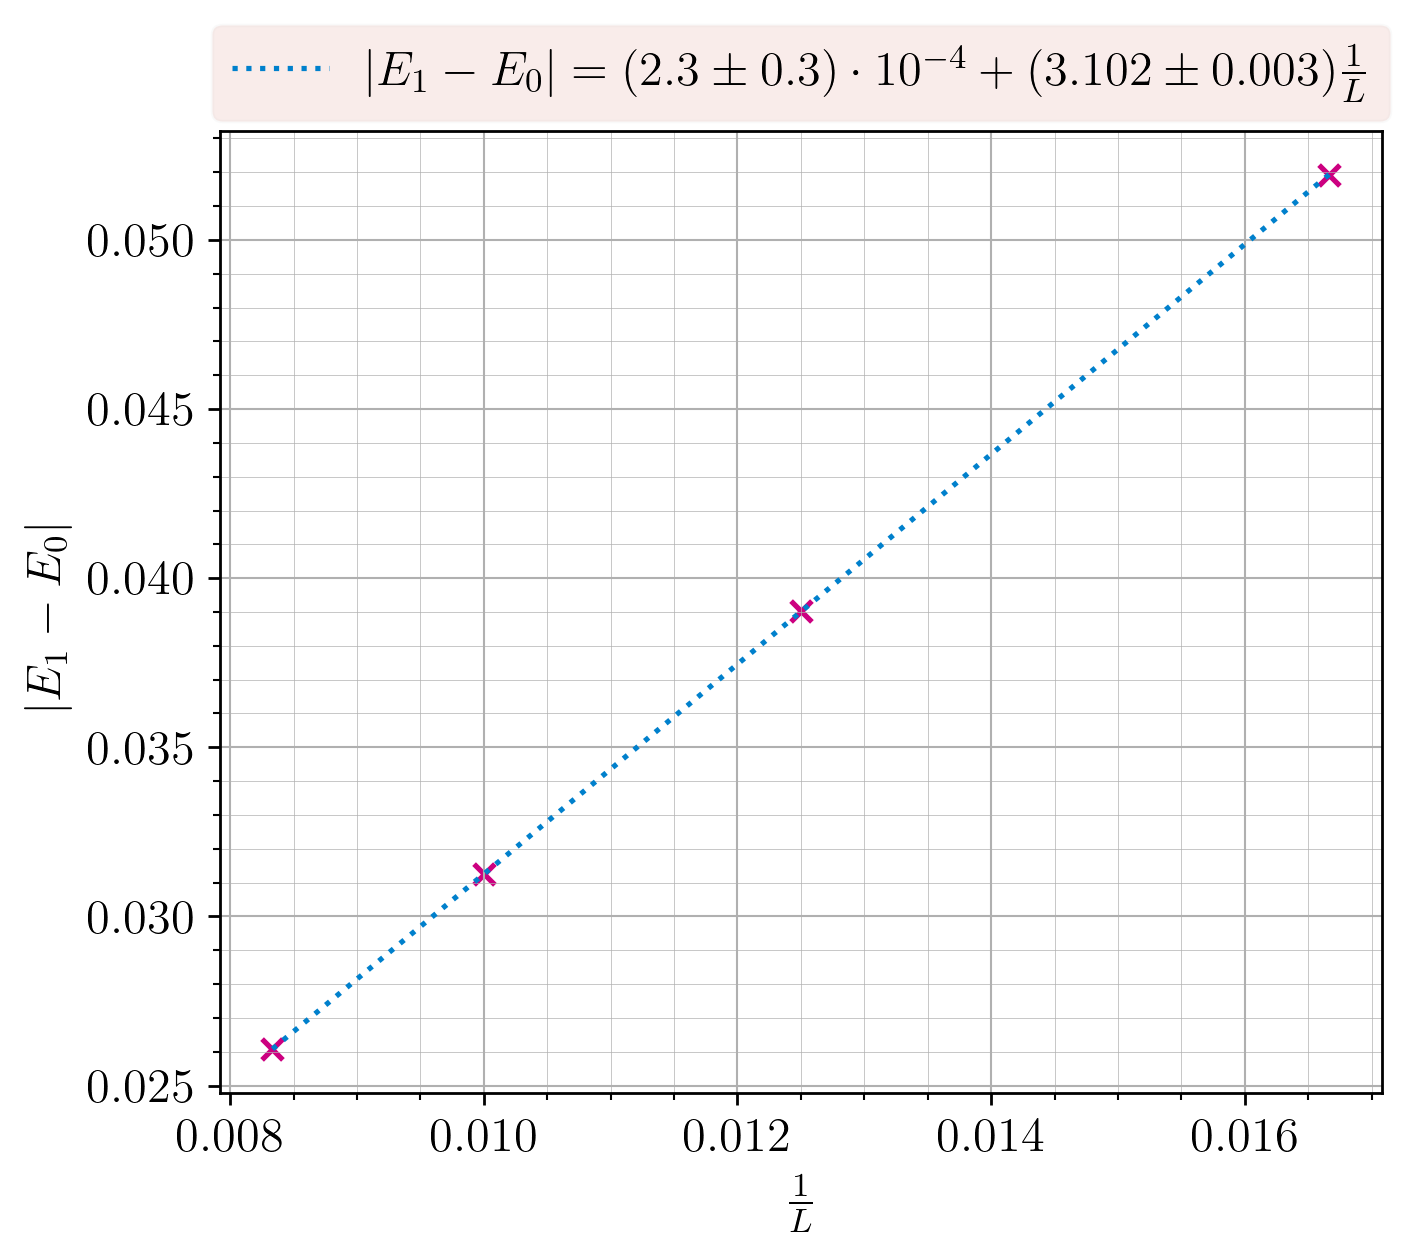
\includegraphics[scale=0.66]{../graphs/gaps/ff/gap_chi=200.0_J=1.0_h=1.0_i=1.0_3=0.0_c=0.0.png}}
		\caption{TFI with $[ff]$ OBCs. (a): Gap between first two non-degenerate energies of TFI for $L=50$ and $\chi=50$ as the field $h$ is varied. (b): Extrapolation of the gap at criticality $J=h$ for $\chi=200$.}
		\label{fig:gapsTFI}
	\end{figure}

	The energy scaling of the ground state has been expressed in \cite{affleck1986} and can be written \cite{blote1986, lassig1991}, once again following \cite{chepiga2017},
	\be E_0 = \varepsilon_0 L + \frac{\pi v}{L}\left[\Delta -\frac{1}{48}\right] + \varepsilon_1 \label{eq:gsScaling} \ee
	where $v = \frac 1 2$ for Ising CFT \cite{affleck1986}, $\varepsilon_0, \varepsilon_1$ non-universal fitting parameters to account for finite size effect and $\Delta$ the conformal dimension of the primary field of the Ising CFT, or the minimum conformal dimension if there is a superposition of several towers. For Ising CFT, there are $3$ fields realized via some OBCs and are given in \autoref{tab:isingConfDim} \cite{cardy1986, cardy1989, francesco1997}. Moreover, the $[ff]$ condition is realized via superposition of $\one$ and $\varepsilon$.

	\begin{table}[h!]
		\centering
		\renewcommand{\arraystretch}{1.3}
		\begin{tabular}{ccc}
			Operator & Dimension & Realization \\
			\hline
			$\one$ & $0$ & $[++]\ [--]$ \\
			$\varepsilon$ & $\frac 1 2$ & $[+-]\ [-+]$ \\
			$\sigma$ & $\frac{1}{16}$ & $[f-]\ [f+]\ [-f]\ [+f]$ \\
			\hline
		\end{tabular}
		\caption{Different CFT operators realized with corresponding boundary conditions and their dimension, used for the construction of the conformal towers..}
		\label{tab:isingConfDim}
	\end{table}

	Therefore, the scaling of ground state energy of critical TFI is presented on \autoref{fig:gsSalingTFI}, where only one realization of each operator is shown and $v\sim 1/2$ quite precise for all of them. Each time, the ground state energy if fitted with \eqref{eq:gsScaling} to find $\varepsilon_0$ and $\varepsilon_1$, and where $v$ can also be computed. Then a linear regression is performed of $\frac{E_0 - \varepsilon_1}{L} - \varepsilon_0$ against $1/L^2$ for a neat view and where the intercept is found to be negligible, as wanted.

	\begin{figure}[h!]
		\hspace{-0.5cm}
		\begin{minipage}{\linewidth}
			\subfloat[]{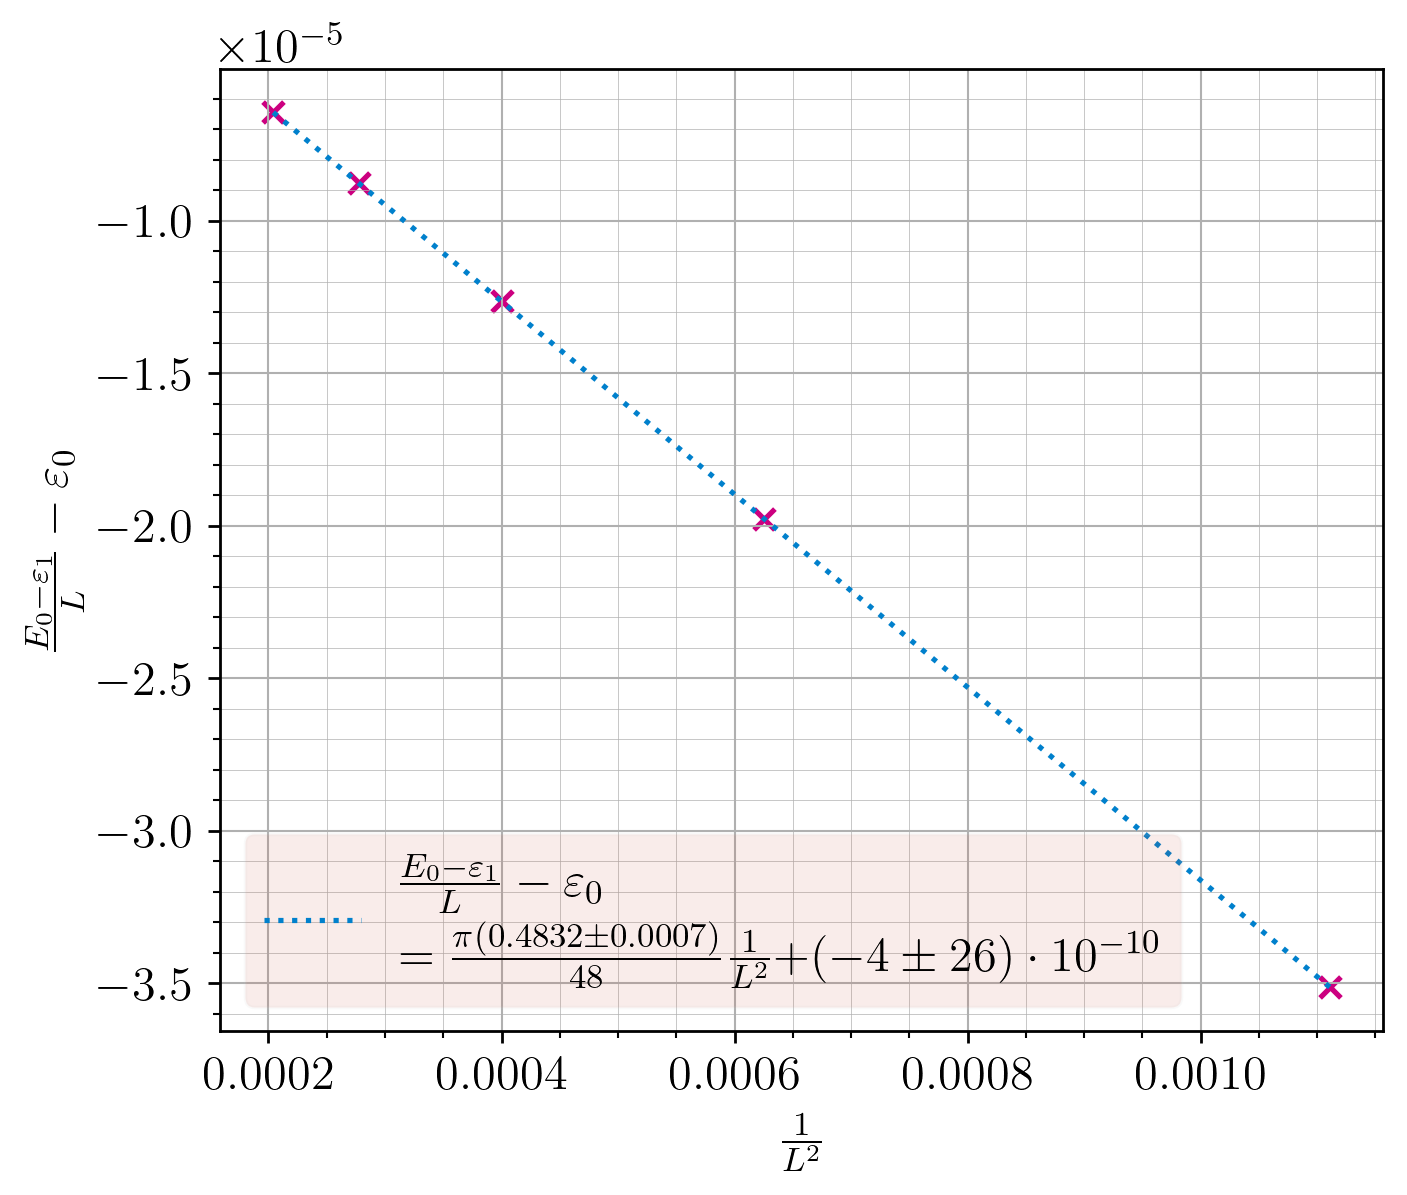
\includegraphics[scale=0.66]{../graphs/conformal/ff/gs_chi=50.0_J=0.25_h=0.25_i=0.5_3=0.0_c=0.0.png}}\
			\subfloat[]{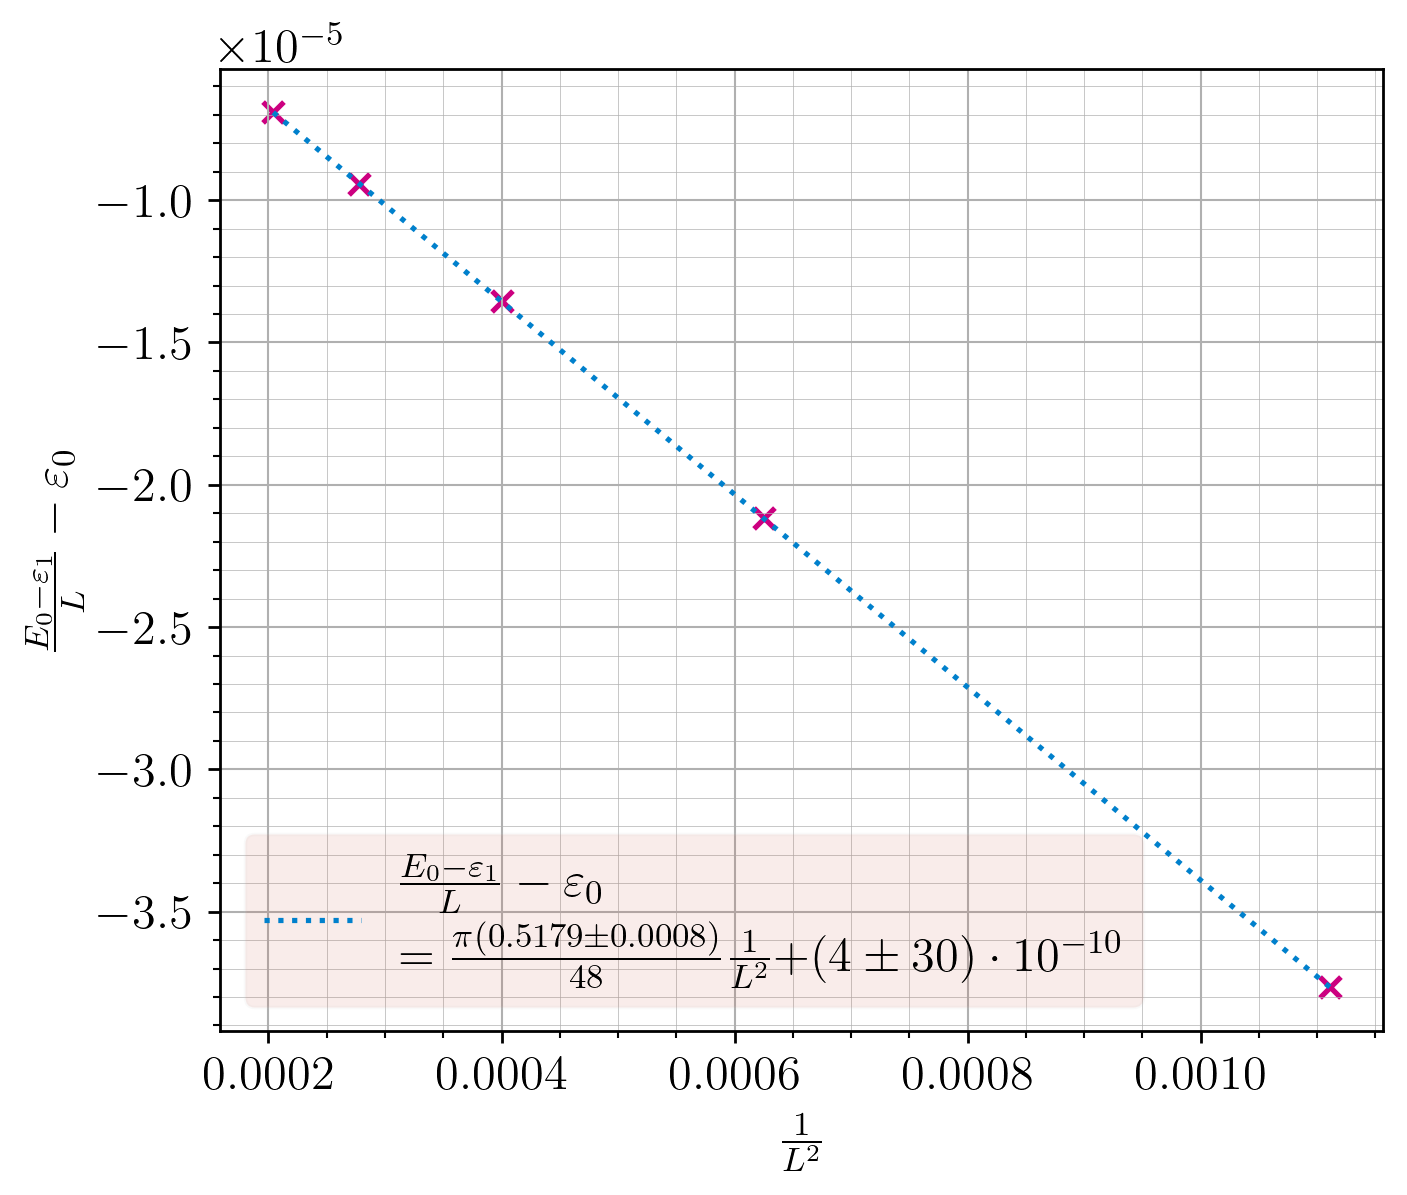
\includegraphics[scale=0.66]{../graphs/conformal/100/--/gs_chi=50.0_J=0.25_h=0.25_i=0.5_3=0.0_c=0.0.png}}
		\end{minipage}

		\hspace{-0.5cm}
		\begin{minipage}{\linewidth}
			\subfloat[]{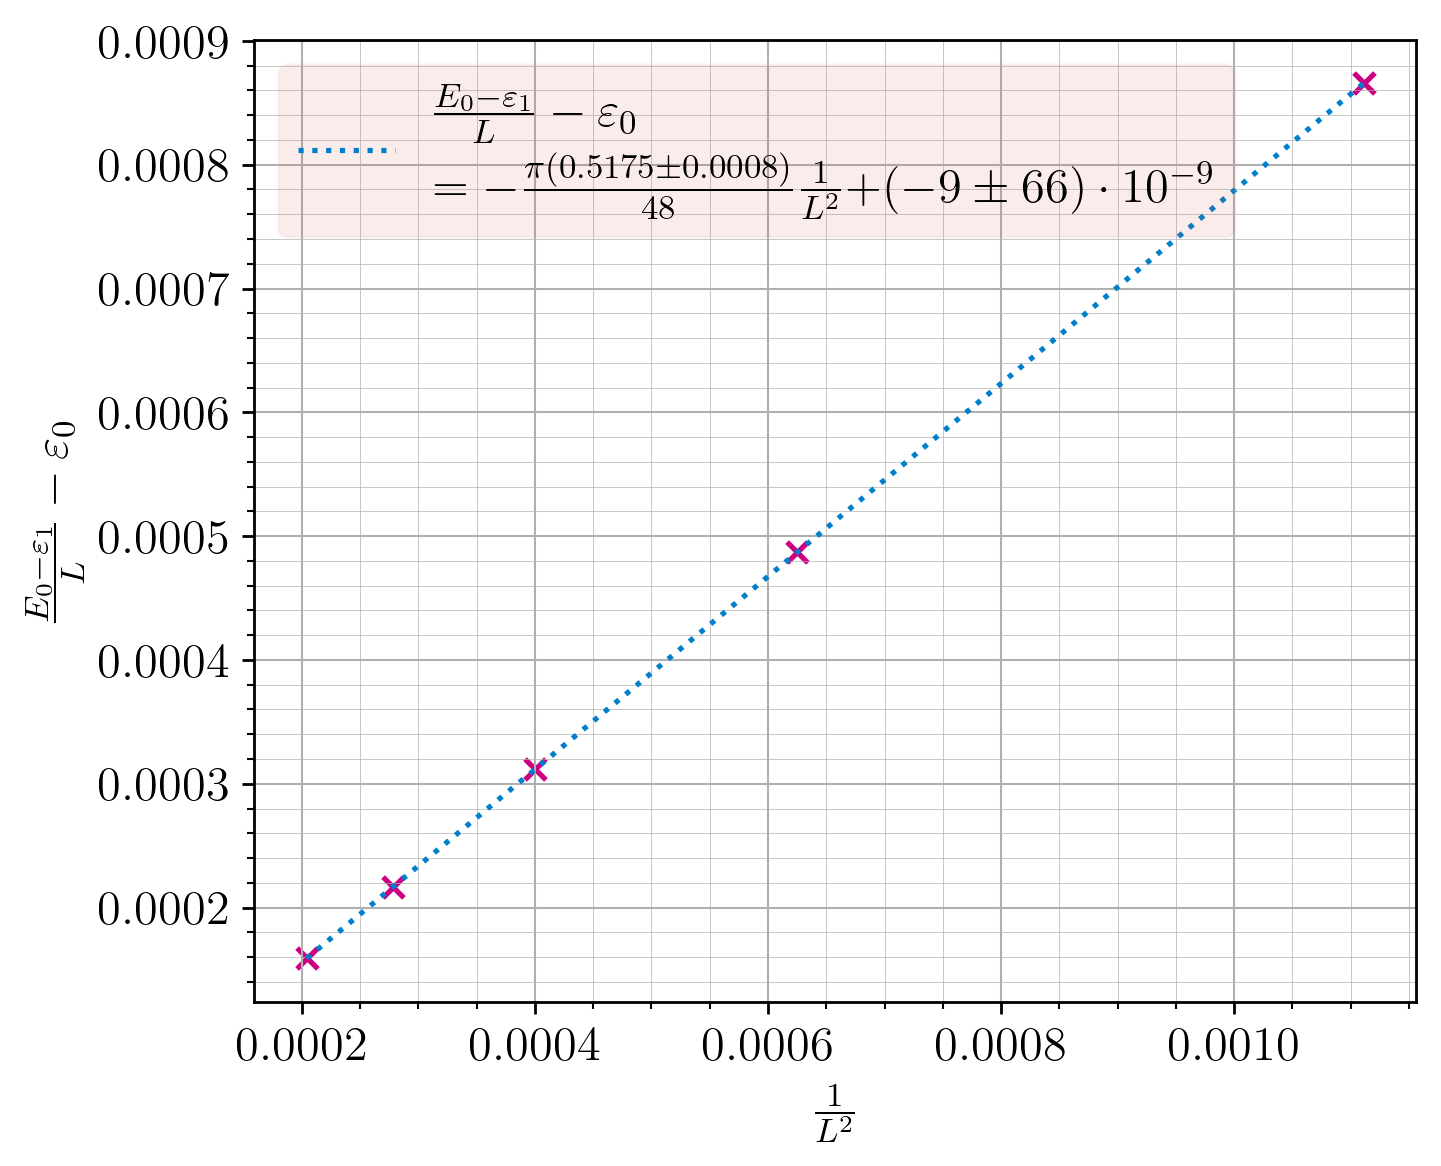
\includegraphics[scale=0.66]{../graphs/conformal/100/+-/gs_chi=50.0_J=0.25_h=0.25_i=0.5_3=0.0_c=0.0.png}}\
			\subfloat[]{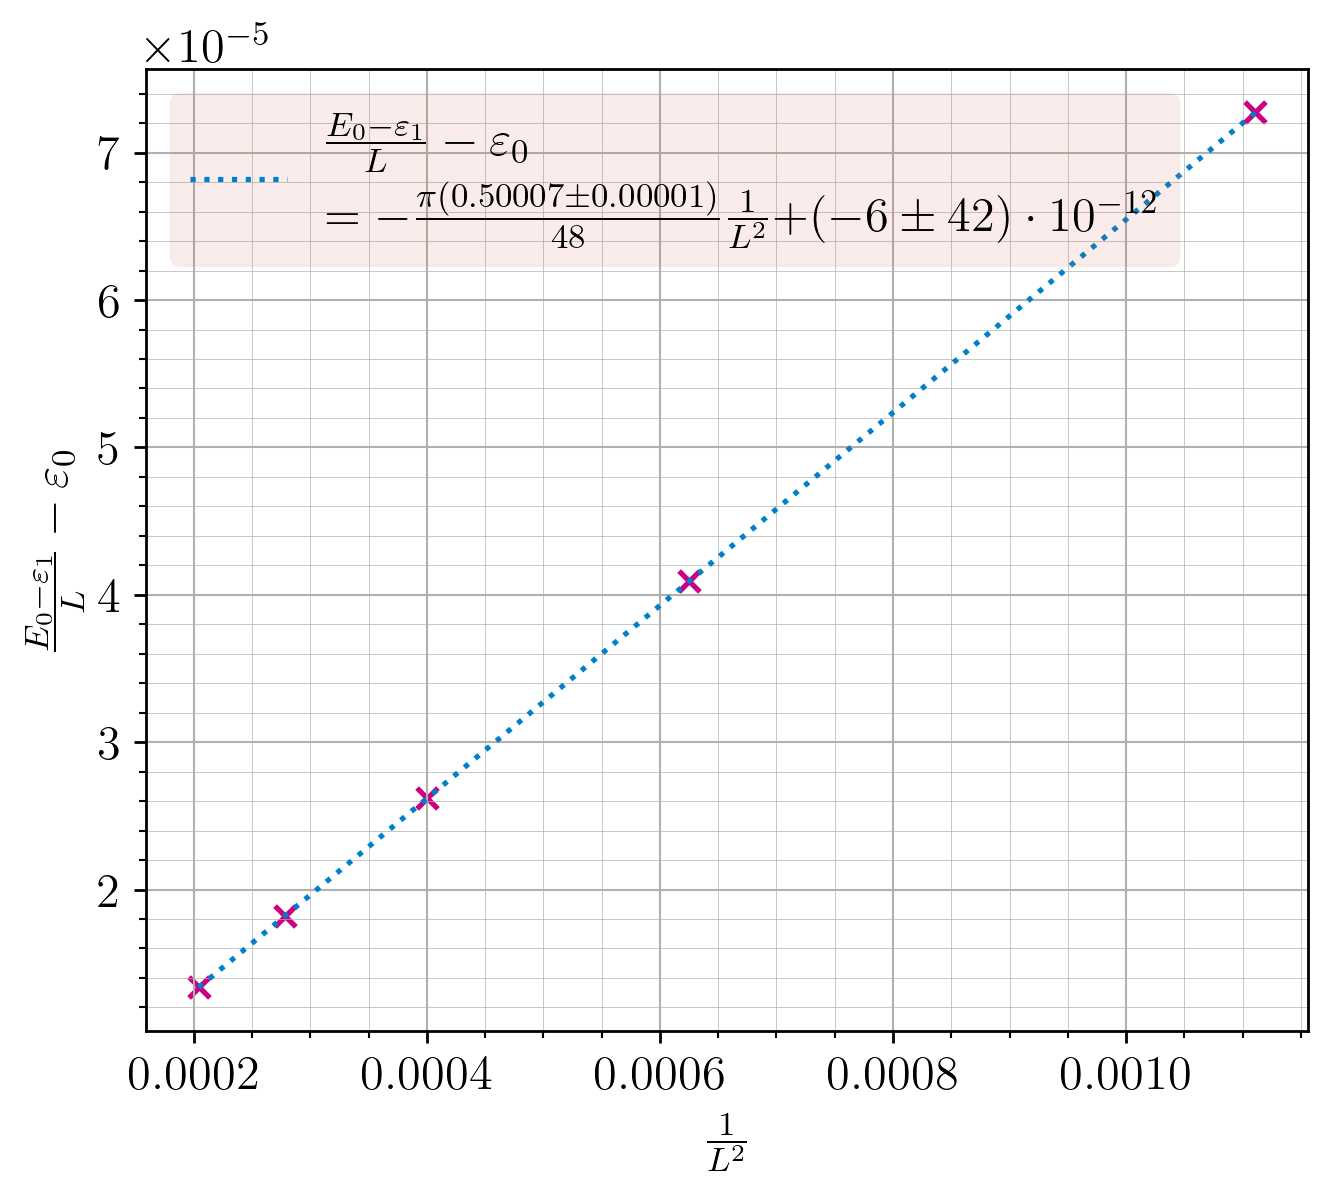
\includegraphics[scale=0.66]{../graphs/conformal/100/f+/gs_chi=50.0_J=0.25_h=0.25_i=0.5_3=0.0_c=0.0.png}}
		\end{minipage}
		\caption{Ground state energy scaling for critical TFI and $\chi=50$ for (a): $[ff]$ OBCs. (b): $[++]$ OBCs. (c): $[-+]$ OBCs. (d): $[f-]$ OBCs. The coefficient in front of $1/L^2$ depends on the conformal dimension of the operator realizing the OBCs, or on the minimum of them if the OBCs are a superposition of several operators. If not free, each edge has pinning magnitude $|h_\text{pin}|=100$.}
		\label{fig:gsSalingTFI}
	\end{figure}

	The conformal towers are finally observed on \autoref{fig:towersTFI} with $10$ energies computed, again following \cite{chepiga2017}. Each excitation has a certain multiplicity taken from the characters of the irreducible representations of the model \cite{cardy1986, cardy1989, francesco1997} and correspond to the one found for each tower for Ising CFT. The characters are explicitly described in \cite{chepiga2017}. In order in them for each operator gives a line in the figure. It can be seen that they agree very well with the data with the multiplicities -- the coefficient of each order -- found at each level agreeing as well. It has been therefore shown that the way to compute the excitation energies is correct, at least for TFI.

	The construction of the conformal towers for TCI CFT for the point $\lambda_3/\lambda_I$ was wanted to be made, to characterize this point with another way than the central charge  which compellingly seemed to be cursed for OBCs. Moreover, the PBCs could have resolved this problem of central charge, but unfortunately a small and well hidden mistake had been made in the construction of the PBCS MPO for \eqref{eq:OF} and the use of these boundary conditions was about to be dropped. However, being a very beginner, finding the expansion of the characters correctly as well as the realization of the primary field of TCI CFT via some boundary conditions was hard. Some references have been found \cite{affleck2000, belavin1984, cardy1986, cardy1989, friedan1985, friedan1984, lassig1991, qiu1986}, but in the meantime, the PBCs MPO problem has been resolved so the works moved on the use of these PBCs as in \cite{obrien2018}.

	\begin{figure}[h!]
		\hspace{-0.5cm}
		\begin{minipage}{\linewidth}
			\subfloat[]{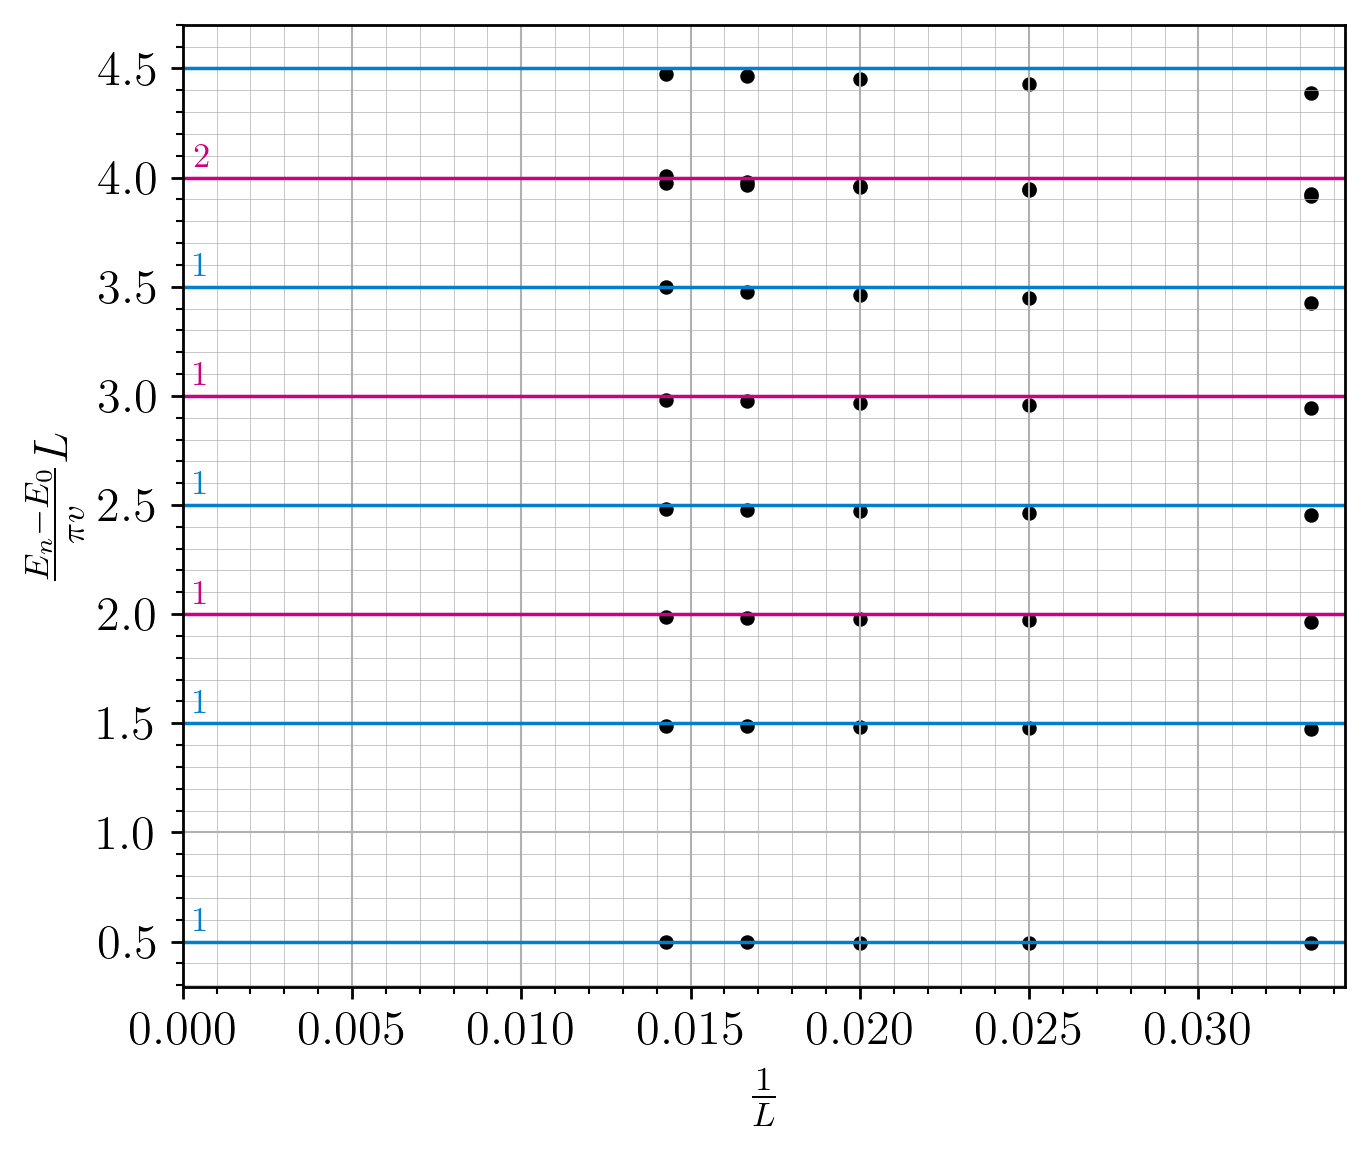
\includegraphics[scale=0.66]{../graphs/conformal/ff/towers_chi=50.0_J=0.25_h=0.25_i=0.5_3=0.0_c=0.0.png}}\
			\subfloat[]{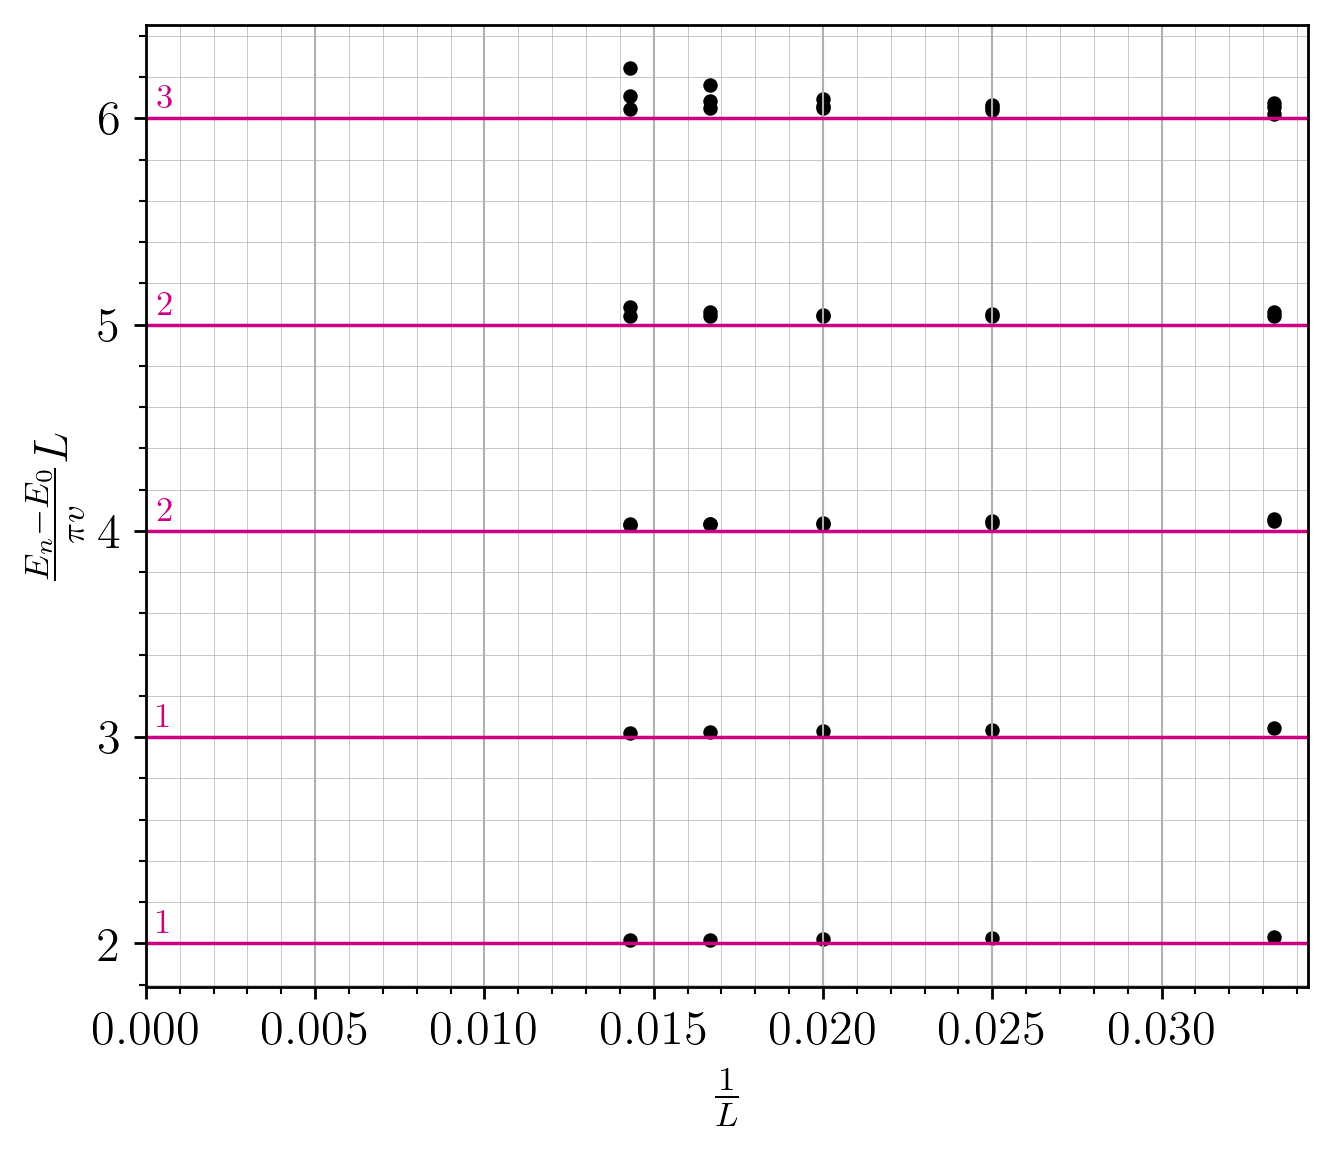
\includegraphics[scale=0.66]{../graphs/conformal/100/--/towers_chi=50.0_J=0.25_h=0.25_i=0.5_3=0.0_c=0.0.png}}
		\end{minipage}

		\hspace{-0.5cm}
		\begin{minipage}{\linewidth}
			\subfloat[]{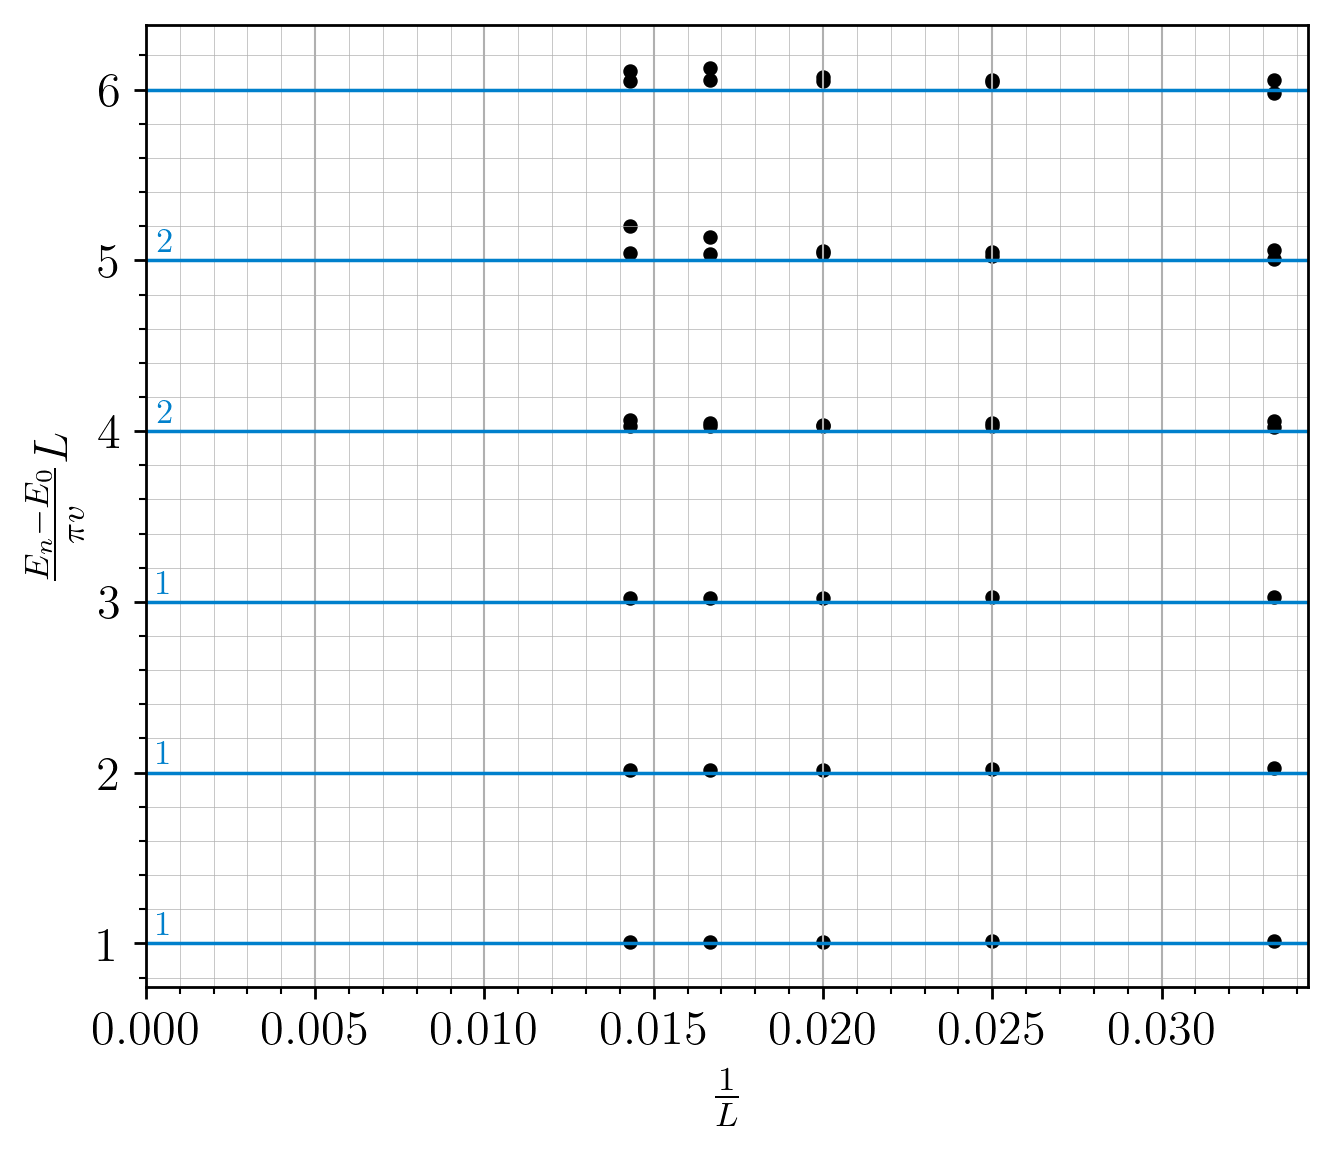
\includegraphics[scale=0.66]{../graphs/conformal/100/+-/towers_chi=50.0_J=0.25_h=0.25_i=0.5_3=0.0_c=0.0.png}}\
			\subfloat[]{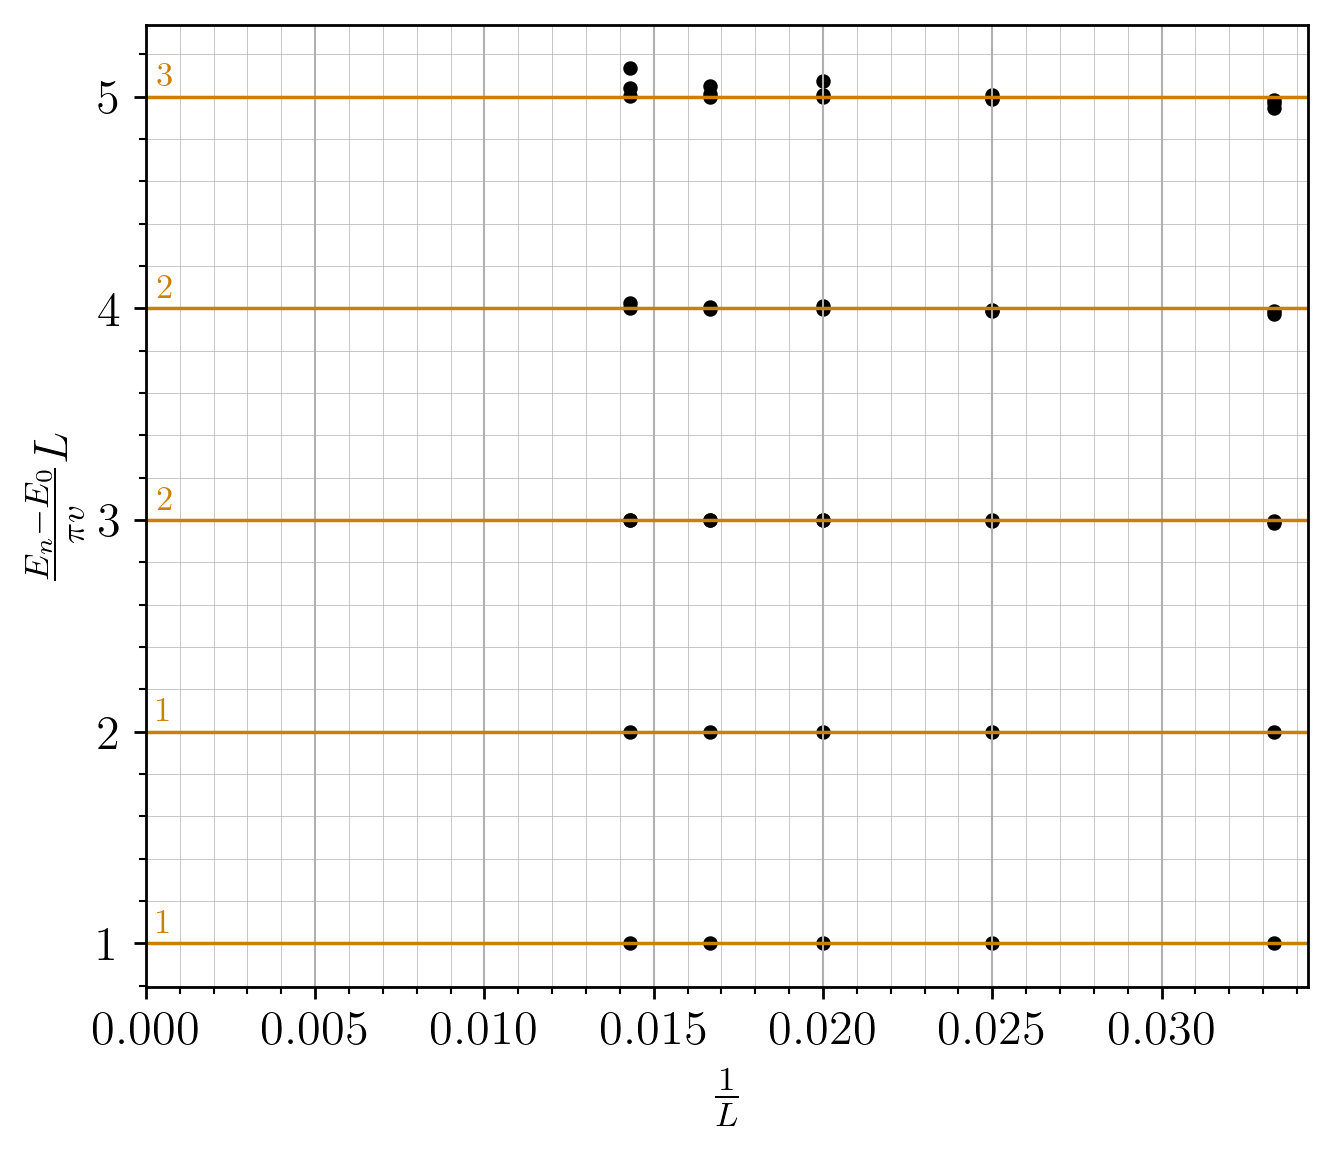
\includegraphics[scale=0.66]{../graphs/conformal/100/f+/towers_chi=50.0_J=0.25_h=0.25_i=0.5_3=0.0_c=0.0.png}}
		\end{minipage}
		\caption{Conformal tower obtained for critical TFI and $\chi=50$ for for (a): $[ff]$ OBCs. (b): $[++]$ OBCs. (c): $[-+]$ OBCs. (d): $[f-]$ OBCs. Black dots represent data. Lines represent predictions from CFT and the numbers the degeneracy obtained for each level. Magenta is for $\mathbb{1}$, cyan for $\varepsilon$ and yellow for $\sigma$. If not free, each edge has pinning magnitude $|h_\text{pin}|=100$. Notice that $v=1/2$ here coming from Ising CFT.}
		\label{fig:towersTFI}
	\end{figure}

	Now that the PBCs work -- at least the correct ground state energy was recovered -- the central charge can be computed, this time using \eqref{eq:cardyPBCs}. It is recovered by extrapolating in $1/L^2$, as it is usually done \cite{milsted2017}, for both critical TFI and OF at $\lambda_3/\lambda_I=0.856$ on \autoref{fig:cPBCs}. A low variance is very difficult to obtain for reasonable bond dimensions, especially for \eqref{eq:OF}, then $\chi$ was chosen each time to reach a descent variance of $\sim 10^{-4}$. Also, it can be observed for critical TFI the extrapolation of $c$ is precise to $10^{-5}$ and even the individual values are in the scale of $10^{-5}$ for quite small lengths between $40$ and $70$. A worse precision is obtained for $\lambda_3/\lambda_I=0.856$ for each individual data and the extrapolation but it is still very acceptable and goes to $c=0.699586\pm0.000008$ being close up to $\sim 10^{-3}$ to $0.7$ expected for TCI CFT. It seems the PBCs completely resolved the problem of the central charge, and it can be conclude, even if no much compelling evidence for now, that since the central charge of the OF model at $\lambda_3/\lambda_I=0.856$ is the one of TCI, this point is effectively in the TCI CFT. Further computation will be made to completely characterize it.

	\begin{figure}[h!]
		\hspace{-0.4cm}
		\subfloat[]{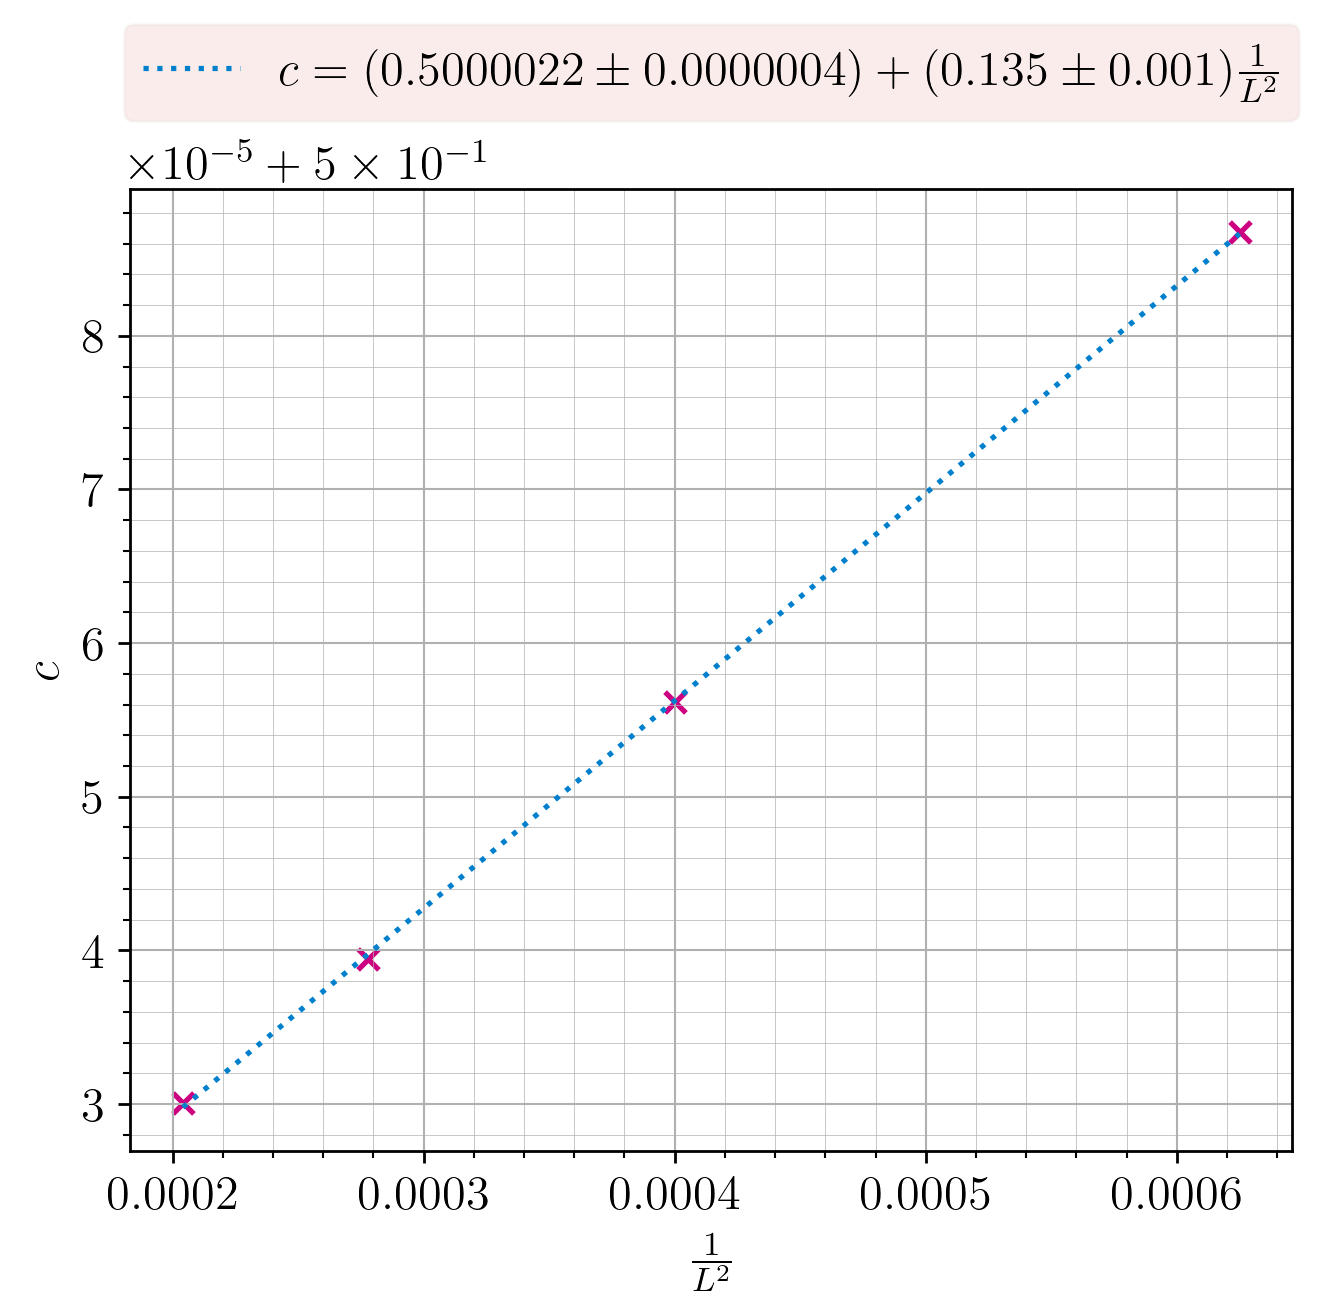
\includegraphics[scale=0.66]{../graphs/entropies/pbc/10-9/calabrese_J=1.0_h=1.0_i=1.0_3=0.0_c=0.0.png}}\quad
		\subfloat[]{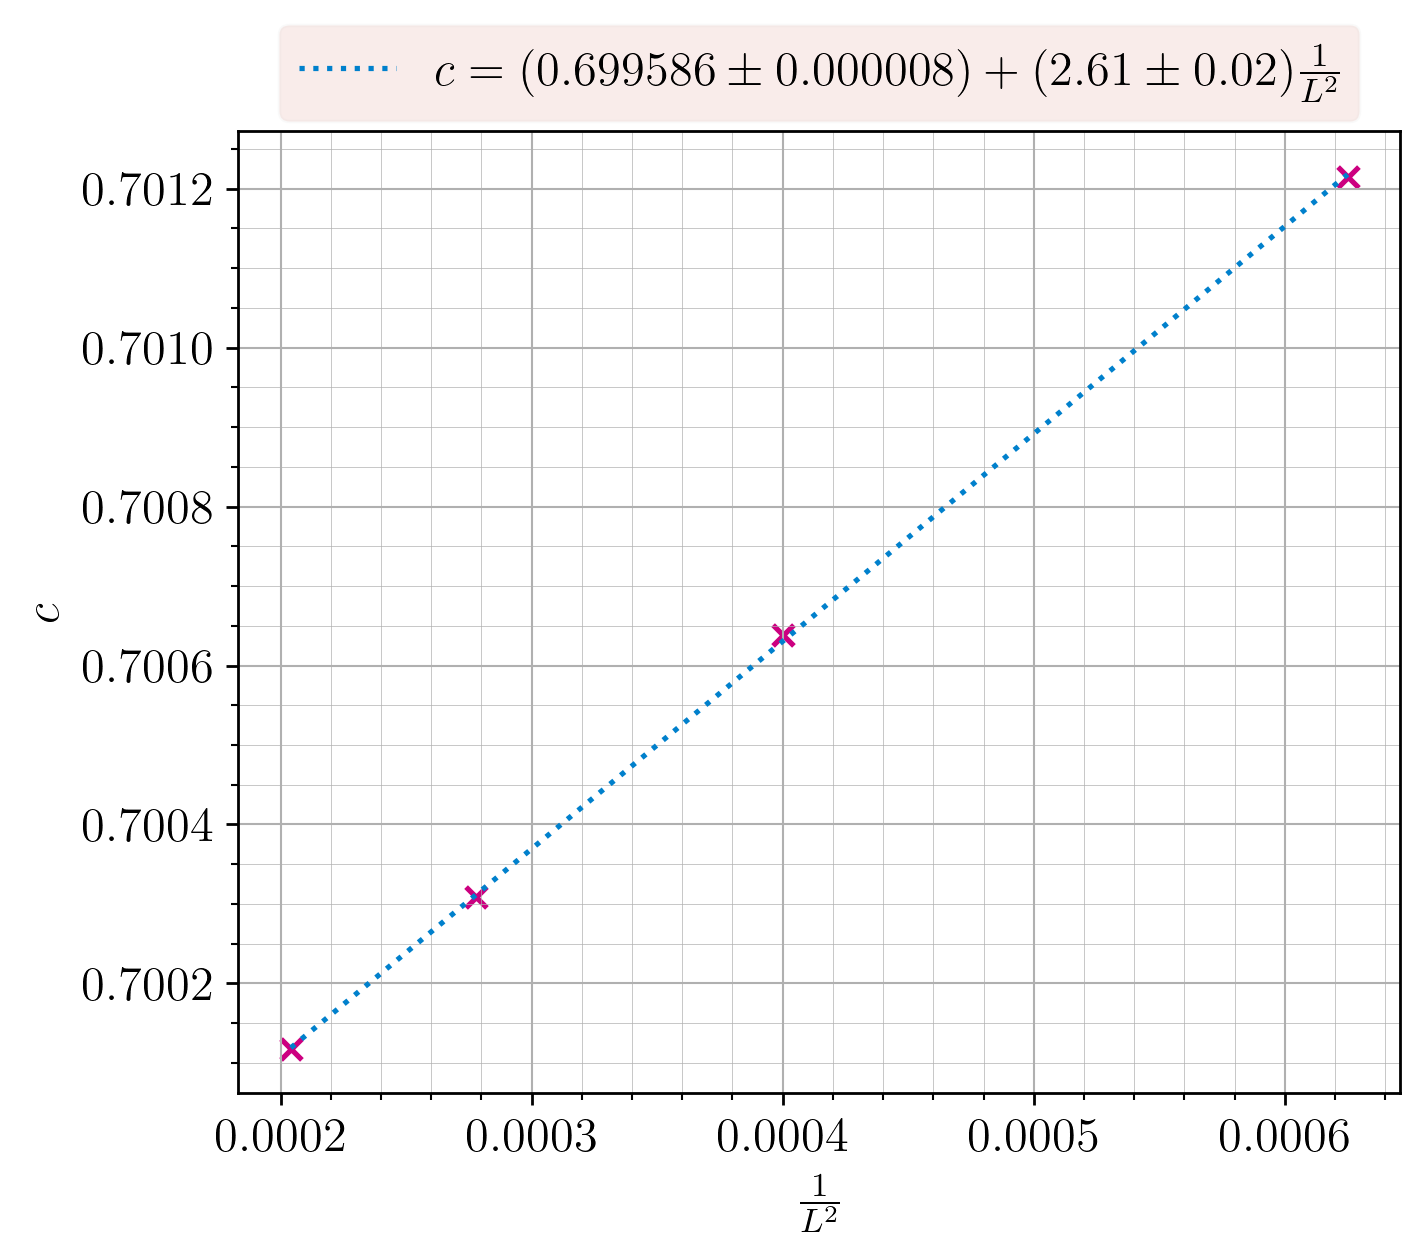
\includegraphics[scale=0.66]{../graphs/entropies/pbc/10-4/calabrese_J=1.0_h=1.0_i=1.0_3=0.856_c=0.0.png}}
		\caption{Extrapolation of the central charge with Cardy-Calabrese formula with PBCs (a): for critical TFI with ground state variance $\sim 10^{-9}$. (b): for $\lambda_3/\lambda_I = 0.856$ with ground state variance $\sim 10^{-4}$.}
		\label{fig:cPBCs}
	\end{figure}

	On \autoref{fig:phasePBCs}, results from \autoref{fig:phaseOBCs} are repeated with PBCs as the ratio $\lambda_3/\lambda_I=0.856$ is varied the see how the central charge behave along this line. This time, the main observation is that the central charge does not reach a maximum before decreasing for $0.7\leq\lambda_3/\lambda_I\leq0.85$, but it monotonically decreasing towards $c\sim 0.5$. The point $\lambda_3/\lambda_I=0.856$ seems to stay at the value $c \sim 0.7$ in $1/L^2$. Consequently, PBCs seem to have resolved the problem of the OBCs.

	\begin{figure}[h!]
		\centering
		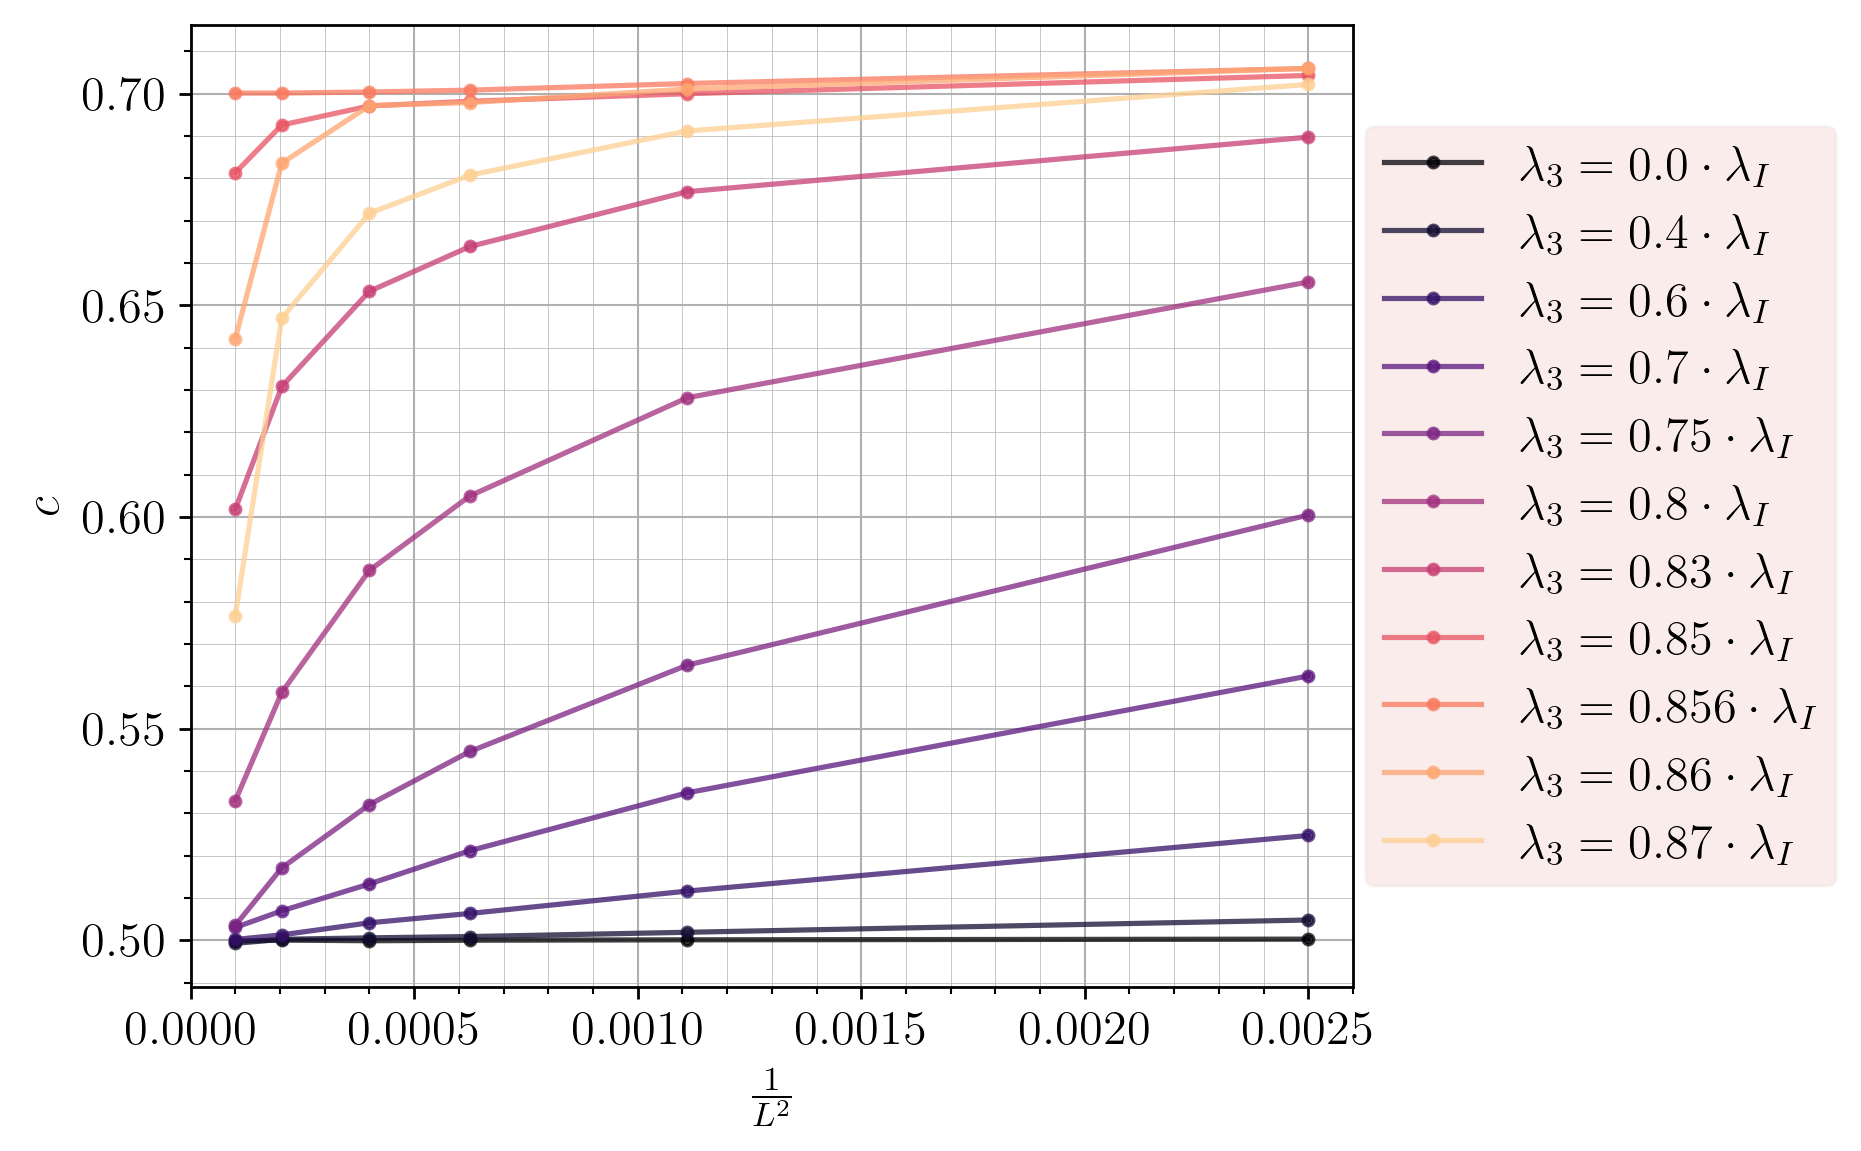
\includegraphics[scale=0.66]{../graphs/phase/pbc/J=1.0_h=1.0_i=1.0_c=0.0.png}
		\caption{Extrapolation of the central charge as $\lambda_3/\lambda_I$ is varied with PBCs for $\lambda_I=1$ and ground state variance $\sim 10^{-4}$.}
		\label{fig:phasePBCs}
	\end{figure}

	To have an insight of what happens at fixed length $L=30$ through the whole interval $\lambda_3/\lambda_I \in [0, 1]$, the central charge in computed for different values of this ratio on \autoref{fig:cWholeInterval}. It can be seen that $c$ is close to $0.5$ for $\lambda_3/\lambda_I<0.6$. Above this, $c$ tends to move aside this $0.5$ and increase towards $0.7$ which is reached for $\lambda_3/\lambda_I$ around $0.856$. After that point, $c$ decrease to reach $0$ approaching $\lambda_3/\lambda_I=1$ as the system there is expected to be gapped. This behavior is for a finite length $L=30$, and it is not excluded that the peak observed around $\lambda_3/\lambda_I=0.856$ narrows as $L$ in increased.

	\begin{figure}[h!]
		\centering
		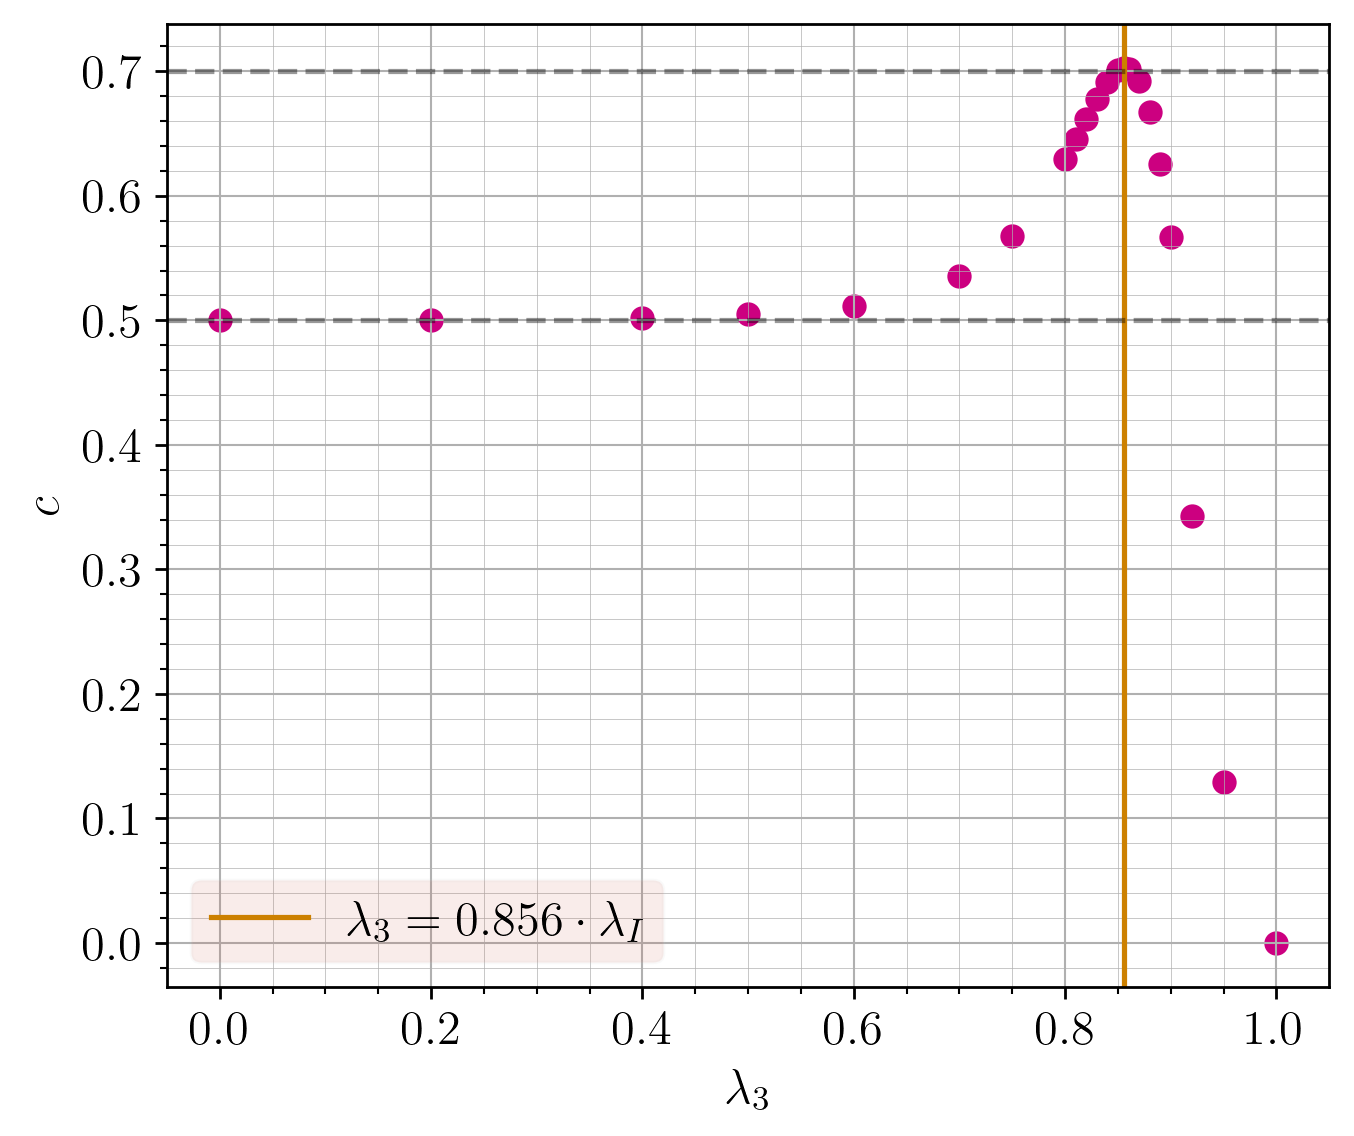
\includegraphics[scale=0.66]{../graphs/through/pbc/L=30.0_chi=100.0_J=1.0_h=1.0_i=1.0_c=0.0.png}
		\caption{Values of central charge as $\lambda_3/\lambda_I$ is varied at fixed length $L=30$, $\chi=100$ and PBCs. Dashed grey lines are added as guides for $c=1/2$ and $7/10$.}
		\label{fig:cWholeInterval}
	\end{figure}

	The use of PBCs was at first intended to compute universal ratios of energies at critical points described by CFT and around to further characterize them. This idea is that ratios of some energy differences are equal to ratios of conformal dimensions difference of the CFT operator realizing the state with the corresponding energy. This is somehow the same idea than building the conformal tower, except there is no need to use a lot of excitation energies and can use PBCs and ABCs. Hence, this will be entirely based on \cite{obrien2018, rahmani2015}. Three ratios will be computed numerically, have been listed in \cite{obrien2018} and are summarized in \autoref{tab:ratios}. The same notation will be used, namely $P^\pm_n$ and $A^\pm_n$ stand respectively for the $n^\text{th}$ excitation PBCs and ABCs energy in the $\pm$ sector of the Hamiltonian \eqref{eq:OF} corresponding to the eigenvalue of the parity operator $\mc F$.

	The results are presented on \autoref{fig:ratios} for different key values of $\lambda_3/\lambda_I$. The length goes from $10$ to $50$, due to the increase in computational cost from PBCs and from the application of the parity operator -- which tends to double the time needed for the same precision. The obtained ratios perfectly agree with those found in \cite{obrien2018} for the same range of lengths. For critical TFI, all values stay on the predicted line even for very small chains. The point $\lambda_3/\lambda_I=0.856$ is slightly off the predicted value for small lengths $10\to 30$ but the precision increases as $L$ increases. Just around it, $\lambda_3/\lambda_I=0.855, 0.857$, they seems to closely follow the behavior of $0.856$ still for small lengths. But starting from $L=30$, they move away from the TCI CFT and $0.855$ initiate its decrease towards Ising CFT, as does $0.8$ neatly, while $0.857$ start to follow a divergent curve as does $0.87$ as expected from $3$-fold degeneracy of the ground state in the gapped phase where $P^+_1 = P^+_0$. This will now be shown.

	\begin{table}[h!]
		\centering
		\renewcommand{\arraystretch}{1.3}
		\begin{tabular}{c|ccc}
			CFT & $R_1 = \frac{A^-_0 - P^+_0}{P^+_1 - P^+_0}$ & $R_2 = \frac{P^-_0 - P^+_0}{P^+_1 - P^+_0}$ & $R_3 = \frac{P^-_1 - P^+_0}{P^+_1 - P^+_0}$ \\
			\hline
			Ising & $\frac{1}{2}$ & $\frac{1}{8}$ & $\frac{9}{8}$ \\
			TCI & $\frac{7}{2}$ & $\frac{3}{8}$ & $\frac{35}{8}$
		\end{tabular}
		\caption{Values of the universal ratios of energy computed from corresponding CFT.}
		\label{tab:ratios}
	\end{table}

	\begin{figure}[h!]
		\centering
		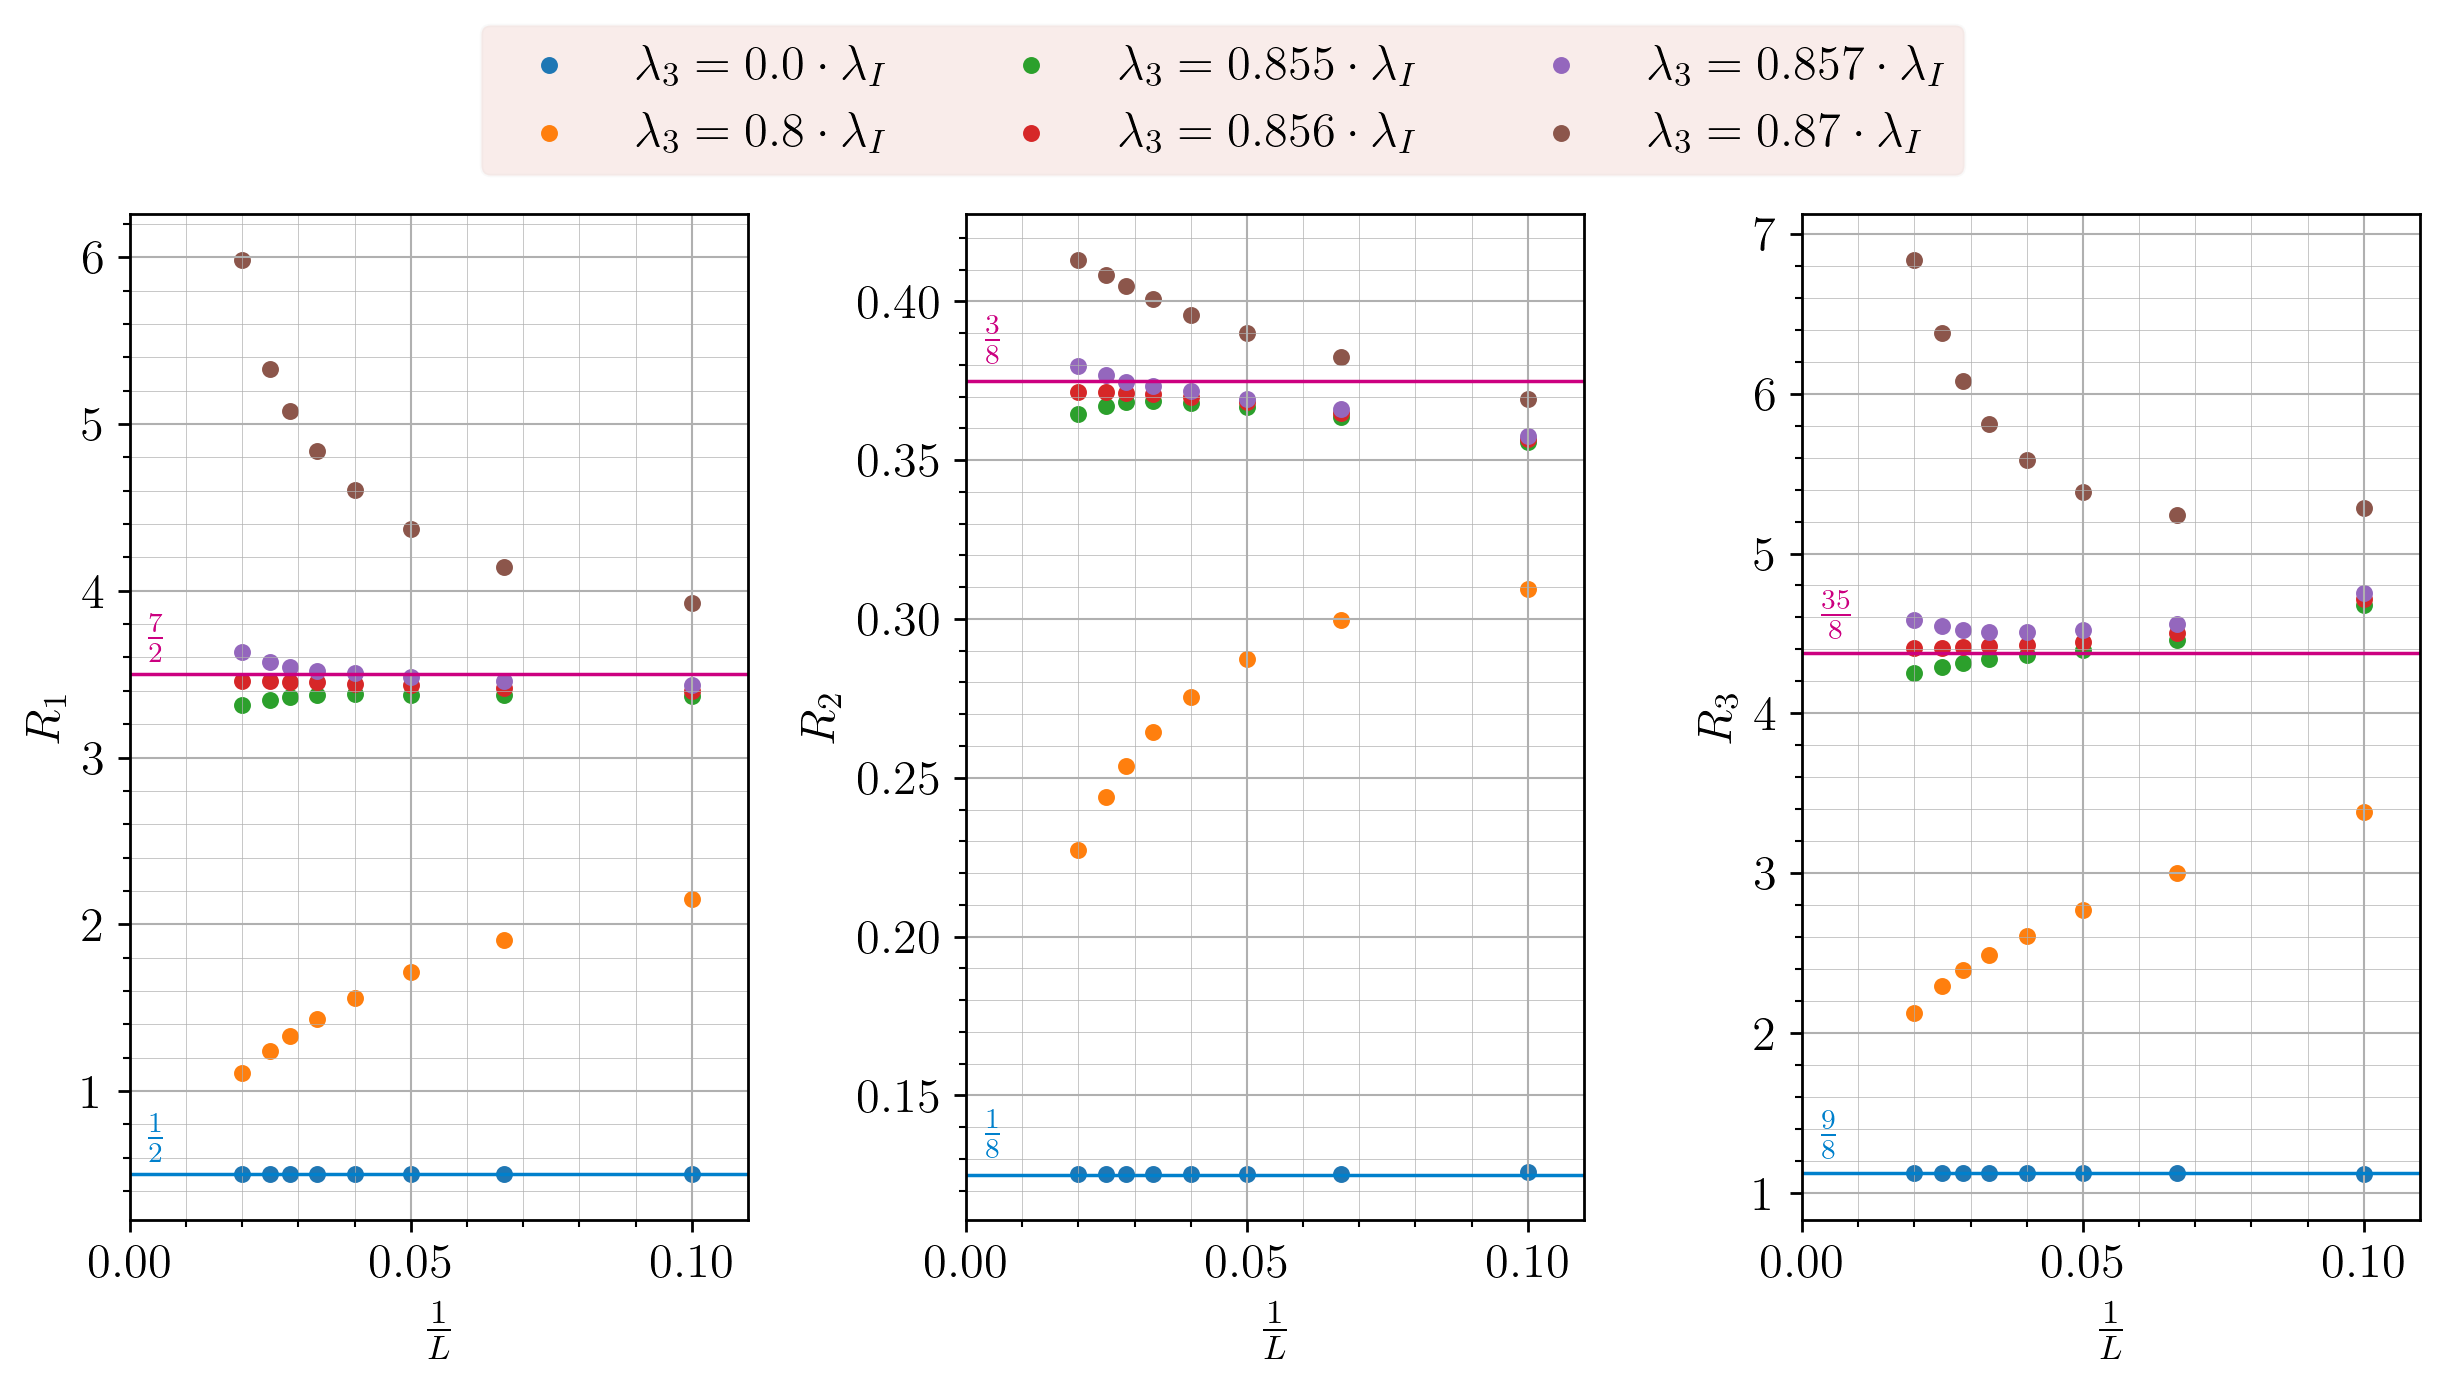
\includegraphics[scale=0.66]{../graphs/ratios/J=1.0_h=1.0_i=1.0_c=0.0.png}
		\caption{Extrapolation of the ratios \autoref{tab:ratios} for different key values of $\lambda_3/\lambda_I$ with ground state variance $\sim 10^{-4}$. CFT prediction are added with their corresponding values : cyan lines are for Ising CFT and magenta lines are for TCI CFT.}
		\label{fig:ratios}
	\end{figure}

	It has been shown that the ground state for $\lambda_3 = \lambda_I$, three ground states exist \cite{obrien2018}. It can be expected that the first three energies of the system from the ratios are $P^+_0$, $P^+_1$ and $P^-_0$ and since they have been shown to converge to the same value in the thermodynamic limit for $\lambda_3/\lambda_I > 0.856$, the differences between those energies are shown on \autoref{fig:degeneracy}. For $0\leq\lambda_3/\lambda_I \leq 0.856$ the system is critical, hence is gapless. Thus, any extrapolation of some energy difference must vanish as $L\to\infty$. Slightly above $0.856$, even though the system is gapped, finite size effects are expected to affect the energies so that they also tend to close the gap for large $L$. As $\lambda_3/\lambda_I$ is increased, only $2$ differences vanish for large lengths -- $P^-_0 - P^+_0$ and $P^+_1 - P^+_0$ --, whereas $P^-_1 - P^+_0$ stops at a finite value, indicating a gap. Since $P^-_1$ has been found to be the $4^\text{th}$ energy, this implies a $3$-fold degeneracy of the ground state for $\lambda_3/\lambda_I > 0.856$. It indeed has been checked that the ground states obtained for $\lambda_3=\lambda_I$ are $\ket{+\cdots +}$ and $\ket{-\cdots -}$ with the exact same energy $E_0 = -2\lambda_I L$. However, there is a third ground state that is not representable in MPS form, as described in \cite{obrien2018}.

	\begin{figure}[h!]
		\centering
		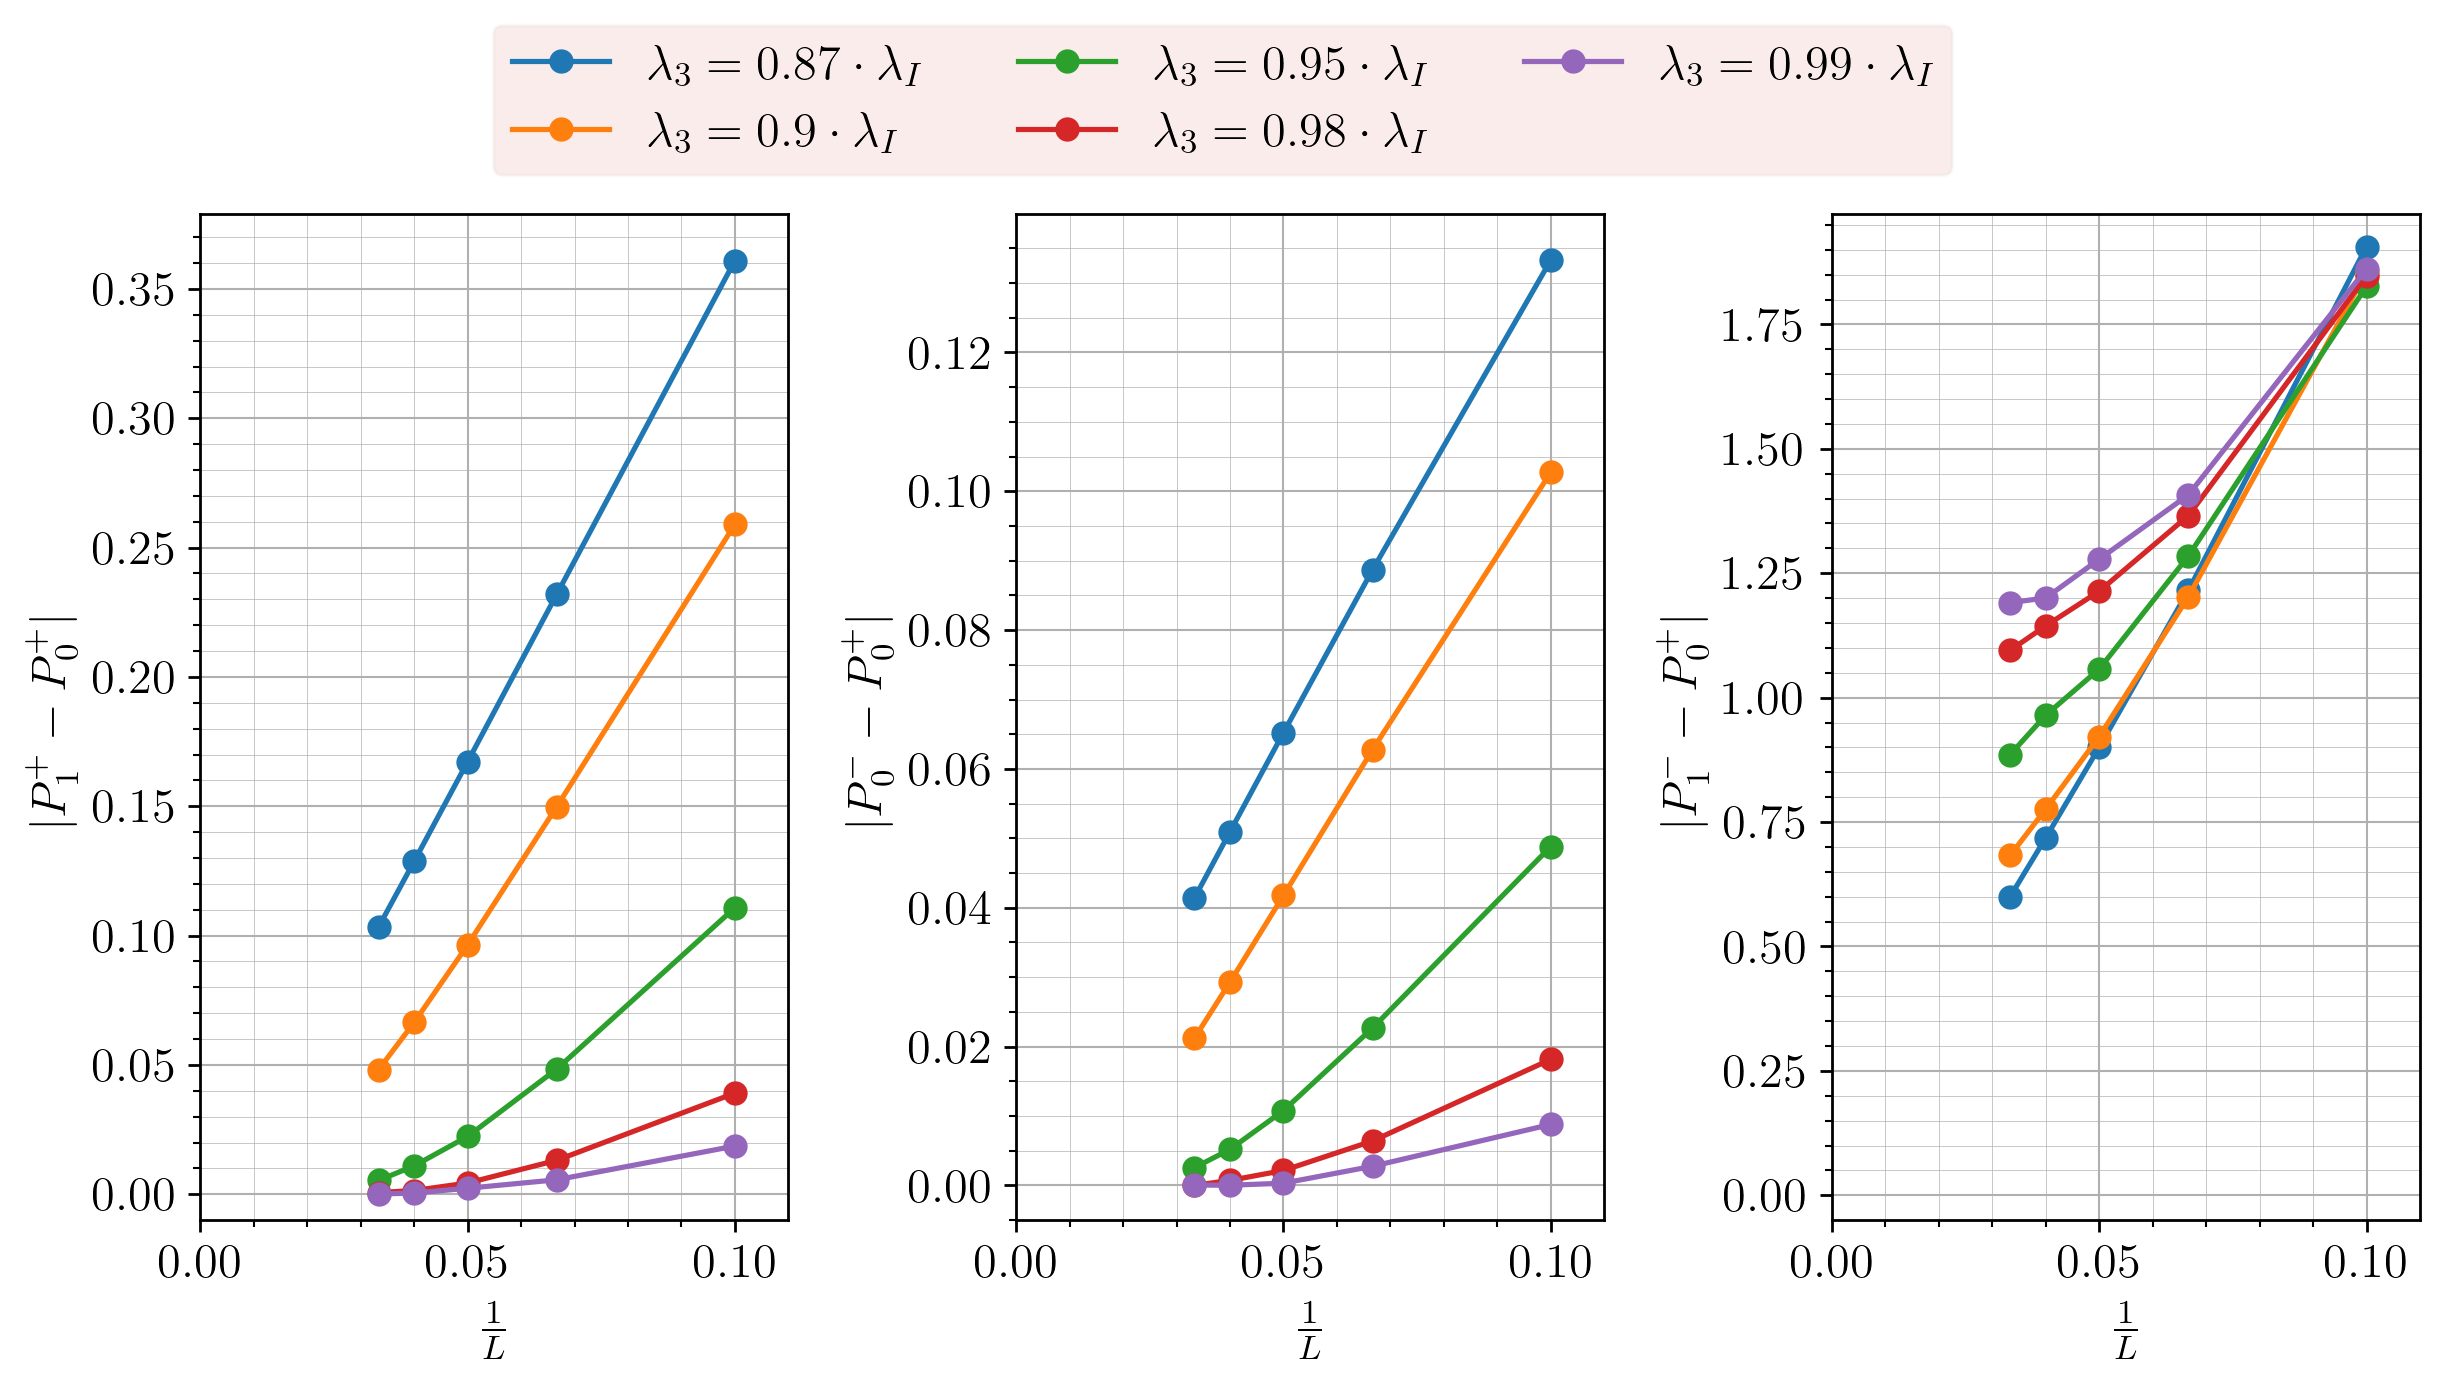
\includegraphics[scale=0.66]{../graphs/degeneracy/J=1.0_h=1.0_i=1.0_c=0.0.png}
		\caption{Extrapolation of the differences in energies for different values of $\lambda_3/\lambda_I$ with ground state variance $\sim 10^{-4}$. Each of them is chosen so that they compose the first low-lying excitation energies.}
		\label{fig:degeneracy}
	\end{figure}
% \clearpage
\section{Conclusion}

	Throughout this project, several aspect of computational quantum physics have been learned. Firstly, the implementation of DMRG enabled to understand deeper the idea underlying the MPS formalism as well as the ground state search using DMRG. Secondly, the extraction of excitation energies in a very efficient way for critical system. Moreover, controlling the convergence to the ground state via the application of some parity operator or the pinning of the edge spins. Finally, the construction of the MPO for Hamiltonian and how to use the DMRG with periodic boundary conditions in an computationally inefficient way but that does not require any change in the code except the calculation of the corresponding MPO Hamiltonian.

	

% \clearpage
\printbibliography

\end{document}